\documentclass[a4paper,polish,titlepage,12pt]{report}
\oddsidemargin 1.0cm
%\textwidth 15.2cm
\usepackage[T1]{fontenc}
\usepackage[polish]{babel}
\usepackage{polski}
\usepackage{textcomp}
\usepackage[utf8]{inputenc}
\usepackage{fancyheadings}
\usepackage[final]{graphicx}
\usepackage{pslatex}
\pagestyle{fancy}
\lhead{}
\bibliographystyle{unsrt}

\usepackage{times}
\usepackage{hyperref}
\usepackage{xcolor,listings}
\usepackage{array}
\usepackage{color}
\usepackage{textcomp}
\lstset{upquote=true}
%\usepackage{graphicx}
\usepackage{lmodern}
\usepackage{wrapfig}
\usepackage[margin=1.3in]{geometry}
\graphicspath{ {rysunki/} }
\hypersetup{
    colorlinks=true, %set true if you want colored links
%    linktoc=all,     %set to all if you want both sections and subsections linked
    linkcolor=blue,  %choose some color if you want links to stand out
    colorlinks,
    citecolor=blue,
    filecolor=blue,
    urlcolor=blue
}

\begin{document}

\begin{titlepage}
\begin{center}
{\small\sc Politechnika Wrocławska, Wydział Informatyki i Zarządzania}\\
\vspace{2.5in}
{\Large Kamil Czarnecki}\\
\vspace{10mm}
{\Huge\bf Algorytmy, projekt i realizacja systemu do zarządzania wielokomputerowymi serwerami WWW}\\
\vspace{1in}
{\large promotor: Prof. Dr hab. inż. Leszek Borzemski}\\
{\large konsultant: Mgr inż. Radosław Porczyński}\\
\vspace{2in}
{\sf Wrocław, 2001}
\end{center}
\end{titlepage}

\begin{titlepage}
\chapter*{}
\begin{Large}
\vspace{15cm}
\hspace{6cm}\emph{prac� dedykuj� Moim Rodzicom}
\end{Large}
\end{titlepage}

%\begin{titlepage}
%\chapter*{}
%\begin{large}
%\vspace{10cm}
%\hspace{2cm}\emph{Serdecznie Dzi�kuj�}

%\hspace{4cm}\emph{\bf }

%\hspace{4cm}\emph{za promotorstwo i wszechstronn� pomoc}

%\hspace{4cm}\emph{\bf }

%%\hspace{4cm}\emph{za wsparcie i pomoc}

%%\hspace{4cm}\emph{\bf }

%\hspace{4cm}\emph{za wyrozumia�o��, wsparcie i du�� pomoc}

%\hspace{4cm}\emph{\bf Hannie Wanzel}

%\hspace{4cm}\emph{za cierpliwo��, wyrozumia�o�� i wsparcie}

%%\end{large}
%%\end{titlepage}


\tableofcontents

\chapter{Wprowadzenie. Cel pracy}
\label{r01}
Celem pracy jest zaprojektowanie i realizacja systemu do zarz�dzania wielokomputerowymi
serwerami WWW oraz przedstawienie ca�okszta�tu tematyki w zakresie r�wnowa�enia obci��e� 
system�w wielokomputerowych i problematyki z tym zwi�zanej.

Dzia�anie og�lno�wiatowej sieci rozleg�ej -- Internetu, rozumiane jest jako ,,lu�no zorganizowana 
mi�dzynarodowa wsp�praca autonomicznych, po��czonych ze sob� sieci komputerowych, w oparciu o komunikacj� 
host--to--host poprzez dobrowoln� przynale�no�� do otwartych protoko��w i procedur zdefiniowanych w dokumentach 
Internet Standards, RFC 1310, RFC1311 i  RFC 1312''. 

Pocz�tk�w Internetu nale�y szuka� w projektach realizowanych na zlecenie Departamentu Obrony USA przez agencj� 
ARPA (ang. \emph{Advanced Research Projects Agency}) oraz jej nast�pczyni� -- agencj� DARPA (ang. \emph{Defense Advanced 
Research Projects Agency}). Przed tymi instytucjami postawiono zadanie opracowania standard�w umo�liwiaj�cych 
budow� rozleg�ej sieci komunikacyjnej odpornej na unicestwienie nawet poprzez atak nuklearny znacznej cz�ci 
jej w�z��w \cite{barylo1}. W wyniku prowadzonych prac w roku 1971 przekazana zostaje do u�ytku sie� ARPANET. Stosowane w niej 
protoko�y transmisji nie zapewnia�y jednak wystarczaj�cej przepustowo�ci dla stale rosn�cej liczby u�ytkownik�w
i ju� w roku 1973 pojawiaj� si� propozycje pierwszych protoko��w z rodziny TCP/IP -- \emph{de facto} dzisiejszego
standardu transmisji internetowych. W roku 1981 na bazie ARPANET--u utworzona zostaje CSN (ang. \emph{Computer Science 
Newtwork})  wykorzystywana wsp�lnie przez abonent�w wojskowych i cywilnych. W roku 1982 
protoko�y TCP/IP wypieraj� ca�kowicie starsze protoko�y (np. protok� NCP),  a do CSN �rednio co 20 dni 
pod��czany jest nowy komputer. W roku 1984 nast�puje podzia� sieci na cz�� wojskow� -- MILNET i cywiln�, 
kt�ra zachowuje tradycyjn� nazw� ARPANET. W miar� jak zaczyna przekracza� ona granice USA i w miar� przybywania 
abonent�w komercyjnych zaczyna pojawia� si� nazwa Internet. W roku 1990 decyzj� rz�du USA szkielet sieci ARPANET 
sk�adaj�cy si� z  czterech w�z��w komutacyjnch (Los Angeles, Santa Barbara, Uniwersytet Stanforda i Uniwersytet 
Utah) zbudowanych w oparciu o minikomputery Honeywell 316 zostaje uznany za przestarza�y i przeznaczony do 
rozbi�rki. Zast�puje go sie� NSFNET, kt�ra do dzi� jest szkieletow� sieci� ameryka�skiej cz�ci Internetu.

Kluczow� ze wzgl�du na tre�� tej pracy dat� w historii Internetu jest rok 1990. Wtedy to w Europejskim O�rodku 
Bada� J�drowych CERN w Genewie zosta� opracowany i uruchomiony pierwszy serwer WWW (ang. \emph{World Wide Web}). WWW 
jest systemem hipertekstowym tzn. przechowuj�cym dane w postaci sieci dokument�w (plik�w) po��czonych poprzez 
odsy�acze. Sam dokument mo�e zawiera� tekst, grafik�, d�wi�k, animacje,  sekwencje video i inne rodzaje danych.  
Elementy wskazywane przez odsy�acze mog� znajdowa� si� w tym samym dokumencie lub by� innymi dokumentami na tym 
samym lub innym serwerze, co dokument zawieraj�cy dany odsy�acz. Obecnie WWW to zbi�r dziesi�tk�w tysi�cy, 
po��czonych sieci� odsy�aczy, serwer�w w wielu krajach. Ka�dy serwer udost�pnia u�ytkownikom zgromadzone na nim 
dokumenty o r�norodnej tre�ci informacyjnej, reklamowej, rozrywkowej, handlowej (e--banki, sklepy internetowe) itp.
Narz�dziem umo�liwiaj�cym zwyk�emu u�ytkownikowi Internetu korzystanie z zasob�w WWW jest przegl�darka
(ang. \emph{browser}). Komunikacja przegl�darki z serwerem WWW odbywa si� w architekturze klient--serwer i jest 
zawsze inicjowana przez zapytania ze strony klienta (przegl�darki). Odpowiadaj�c na zapytania przegl�darki serwer
WWW przesy�a do niej ��dane dokumenty z wykorzystaniem protoko�u HTTP (ang. 
\emph{Hyper Text Transfer Protocol}). Najcz�ciej stosowanym j�zykiem opisu dokumentu hipertekstowego jest HTML 
(ang. \emph{Hyper Text Mark up Language}). Przegl�darka interpretuj�c otrzymany plik HTML potrafi odpowiednio rozmie�ci� 
na ekranie u�ytkownika tekst, grafik� i odsy�acze sk�adaj�ce si� na dokument. Pliki HTML maj�  charakter 
statyczny -- s�u�� do prezentacji wcze�niej przygotowanych danych. Specyfikacja HTML jest jednak bardzo 
elastyczna -- do plik�w HTML mo�na w��cza� skompilowane do postaci kod�w bajtowych programy j�zyka Java, 
skrypty JavaScript, Visual Basic--a czy kontrolki ActiveX, w ten spos�b serwer WWW powoduje uruchomienie w 
komputerze u�ytkownika  program�w przes�anych w dokumencie, co uatrakcyjnia wygl�d dokumentu i umo�liwia pewien 
stopie� dialogu z u�ytkownikiem. Dla zada� takich jak np. wyszukiwanie danych do pliku HTML do��cza� mo�na 
odwo�ania do program�w (skrypt�w) CGI (ang. \emph{Common Gateway Interface}). Program napisany zgodnie z norm� CGI 
wykonywany jest w tym samym komputerze, w kt�rym dzia�a proces serwera WWW -- w takiej sytuacji komputer ten 
staje si� serwerem aplikacji (mo�e r�wnie� prezentowa� dane wydobywane z baz danych).

Nie spos�b m�wi� o serwerach WWW w oderwaniu od takich us�ug internetowych jak 
Gopher, czy serwery FTP, gdy� wiele dokument�w hipertekstowych zawiera odsy�acze inicjuj�ce pobieranie plik�w z 
serwer�w FTP lub dokonuj�cych prze��czenia do systemu Gopher (czysto tekstowego systemu informacyjnego).

Przedstawiana praca dotyczy problematyki rozwoju sieci Internet w zakresie burzliwie rozwijaj�cych si� system�w 
informacyjnych opartych o WWW, a dok�adniej mo�liwo�ci budowy i implementacji wysokowydajnych system�w WWW opartych
o architektur� wieloserwerow�. Tradycyjny system WWW, sk�adaj�cy si� z pojedynczego komputera nie jest w stanie spe�ni�
wymaga� rosn�cej liczby coraz bardziej wybrednych klient�w (zwi�kszanie procesor�w, pami�ci operacyjne i dyskowej w platformach
jednoserwerowych ma swoje granice). Przeci�tny u�ytkownik ,,paj�czyny'' oczekuje w miar� 
szybkiego,
ale przede wszystkim zawsze dost�pnego serwisu internetowego. Maj�c na uwadze fakt, �e systemy WWW stanowi� od pewnego czasu
znakomit� platform� do prowadzenia handlu elektronicznego -- dost�pno�� witryn jest niezb�dna do utrzymania si� na rynku firm 
prowadz�cych tego rodzaju us�ugi. Jedynym, jak si� wydaje, rozwi�zaniem jest tworzenie system�w WWW budowanych
na bazie wieloserwerowej -- tylko takie rozwi�zanie mo�e zapewni� ci�g�� dost�pno�� do zasob�w WWW (ich g��wn� zalet�
jest mo�liwo�� stopniowej i teoretycznie niograniczonej rozbudowy).

Ju� w roku 1995 pakiety HTTP stanowi�y 36\% wszystkich pakiet�w przesy�anych w 
sieci szkieletowej NSFNET \cite{barylo2} i udzia� ten wykazywa� sta�� tendencj� wzrostow�. Obecnie g��wnym motorem rozwoju 
,,�wiatowej paj�czyny'' s� wszelkiego rodzaju e--biznesy (platformy B2B, B2C i inne), co wi��e si� z ogromn� 
integracj� tradycyjnego statycznego HTML--a (lub XML--a) z elementami dynamicznymi zmieniaj�cymi si� w czasie. 
Zwi�ksza to ju� i tak niema�e trudno�ci w optymalnym konstruowaniu serwer�w WWW. W zwi�zku z problemami 
zwi�zanymi z pot�nym przyrostem internaut�w oraz komplikacjami w ci�g�ym rozwijaniu pojedynczych komputer�w 
b�d�cych serwerami WWW, a tak�e wi�zaniu ze sob� r�norakich us�ug internetowych -- stale zwi�kszaj�cym si� 
uznaniem (oraz znakomitym stosunkiem wydajno��/cena) ciesz� si� systemy rozproszone: 
\begin{description}
\item[klastry webowe] -- serwery WWW rozproszone lokalnie tzn. funkcjonuj�ce w obr�bie sieci lokalnej;
\item[rozproszone serwery webowe] -- rozproszone geograficznie serwery webowe pomi�dzy kt�rymi istnieje mechanizm szeregowania;
\item[rozproszone klastry webowe] -- jest to szczeg�lny przypadek rozmieszczenia serwer�w webowych -- stanowi kombinacj� 
globalnego i lokalnego rozproszenia. 
\end{description}
Problemem w ich wykorzystaniu 
jest odpowiednie skierowanie klient�w do najlepszego serwisu tzn. takiego, kt�ry bez wzgl�du na obci��enie jest osi�galny dla 
klienta i zwraca mu odpowied� mo�liwie najszybciej. Aby zrealizowa� tego typu architektur� konieczne jest stworzenie
odpowiednich mechanizm�w szeregowania zapyta� klienckich, algorytm�w szeregowania wyznaczaj�cego najlepszy serwer oraz 
urz�dzenia, w kt�rym jest zaimplementowany mechanizm i algorytm szeregowania. W zale�no�ci od umiejscowienia jednostki
szereguj�cej zapytania od klient�w mo�na wyr�ni� trzy grupy metod:
\begin{itemize}
\item podej�cie: po stronie klienta (wymagaj�ce modyfikacji po stronie klienta -- np.: ingerencji w budow� przegl�darki);
\item podej�cie z wyko�ystaniem niezale�nego w�z�a dystrybuuj�cego zapytania od klient�w (polegaj�ce na modyfikacji lub przekazywaniu
pakiet�w kierowanych do systemu konkretnym serwerom realizuj�cym zlecenie -- np.: komputer z zainstalowanym oprogramowaniem SecureWay Network Dispatcher firmy IBM);
\item podej�cie: po stronie serwera (wymagaj�ce modyfikacji po stronie serwera)
\end{itemize}
Szczeg�owo, zar�wno mechanizmy szeregowania zapyta�, algorytmy szeregowania jak i urz�dzenia, oraz spos�b implementacji tak 
mechanizm�w jak i algorytm�w zostanie szczeg�owo om�wiony w dalszej cz�ci tej pracy (patrz: rozdzia� \ref{r03} i \ref{r04})

Jako przyk�ad systemu o wi�kszej wydajno�ci i dost�pno�ci zaimplementowane zostanie rozwi�zanie oparte o architektur� 
wieloserwerow� w oparciu o komputery IBM RS/6000 pracuj�ce pod kontrol� systemu operacyjnego AIX oraz maszyny typu PC
pracuj�ce pod kontrol� MS Windows NT z wykorzystaniem profesjonalnego oprogramowania r�wnowa��cego obci��enie -- pakietu
IBM SecureWay Nework Dispatcher. 

Celem pracy jest prezentacja algorytm�w i rozwi�za� s�u��cych do zarz�dzania rozproszonymi 
systemami WWW oraz przyk�ad implementacji takiego rozwi�zania. 
Omawiana instalacja serwerowa zosta�a zestawiona w laboratorium Instytutu Sterowania i Techniki System�w 
Politechniki Wroc�awskiej. 

W dalszej cz�ci pracy zostan� przedstawione protko�y TCP/IP, kt�rych znajomo�� jest konieczna do zrozumienia tre�ci zawartych 
w cz�ci praktycznej. Ten kr�tki opis obejmie IP, TCP, UDP, HTTP, FTP, SMTP, SNMP, SSL, DNS, oraz adresowanie URL. Po opisie 
protoko��w zostanie szczeg�owo przybli�ona architektura klient--serwer, struktura WWW oraz klasyfikacja i opis architektur
rozproszonych serwer�w WWW. Kolejny rozdzia� wyja�nia czym jest i do czego jest potrzebne zarz�dzanie wielkomputerowymi 
systemami WWW oraz w jakich sytuacjach si� to zarz�dzanie stosuje. Ostatnim punktem tej pracy jest opis konfiguracji 
przyk�adowego systemu WWW wykorzystuj�cego oprogramowanie IBM Network Dispatcher\footnote{Aktualnie IBM Network Dispatcher jest elementem oprogramowania o nazwie IBM WebSphere Edge Server}.

\chapter{Protoko�y komunikacyjne (sieciowe)}
\label{r02}

W rozdziale tym przedstawiona zostanie architektura ISO/OSI stosu protoko��w, dzi�ki kt�rym wydajna i bezpieczna 
transmisja w sieci nie by�aby w og�le mo�liwa: od protoko��w TCP/IP, poprzez SSL do protoko��w FTP i HTTP. 
Opisany zostanie tak�e spos�b identyfikacji i komunikacji urz�dze� i zasob�w sieciowych na r�nych warstwach 
czyli DNS i URL. Najwi�cej uwagi po�wi�cone zostanie na opis protoko�u HTTP i spos�b dzia�ania WWW.

\section{Wst�p}

Podstawow urz�dzenia komunikacyjne sk�adaj� si� z element�w, kt�re przesy�aj� bity z jednego miejsca do drugiego. Jednak�e
u�ywanie ,,surowego'' sprz�tu do komunikacji jest podobne do programowania przez wrowadzanie zer i jedynek -- jest to 
niepor�czne i niewygodne. Komputery pod��czone do sieci s� wyposa�one w skomplikowane oprogramowanie udost�pniej�ce
wygodny, wysokopoziomowy interfejs dla program�w u�ytkownika. Oprogramowanie to obs�uguje automatycznie wi�kszo�� 
niskopoziomowych szczeg��w oraz problem�w, co pozwala na �atw� komunikacj� mi�dzy programami u�ytkowymi. W ten spos�b
wi�kszo�� program�w u�ytkownika przy komunikacji polega na oprogramowaniu sieciowym i nie komunikuje si� bezpo�rednio ze
sprz�tem.

Wszystkie strony bior�ce udzia� w komunikacji musz� uzgodni� zbi�r regu� u�ywanych przy wymianie komunikat�w. Zbi�r regu�, 
kt�re okre�laj� format komunikat�w, oraz stosownych dzia�a� wymaganych dla ka�dego komunikatu nazywa si� protoko�em sieciowym.

\section{TCP/IP a ISO/OSI}

Aby sprawienie i efektywnie rozwi�za� dowolne zadanie komunikacyjne oraz zaplanowa� zestaw 
protoko��w stworzono model warstwowy \cite{siecikomputerowe}.
Zestaw protoko��w mo�na tym samym zwi�za� z okre�lon� warstw� \cite{barylo1}.

Wcze�nie w historii sieci \emph{International Organization for Stadarization} (ISO) opracowa�a model 7--warstwowy.
Model ISO/OSI jest standardem stanowi�cym punkt odniesienia dla producent�w oprogramowania i sprz�tu sieciowego. 
Stosowanie si� do zalece� tego standardu zapewni� ma kompatybilno�� r�nych produkt�w sieciowych, co implikuje 
mo�liwo�� swobodnego ich ��czenia w tzw. system otwarty.
Wyr�ni� w nim mo�na: warstw� aplikacji, prezentacji i sesji -- nazywane warstwami g�rnymi, oraz
warstw� transportow�, sieciow�, ��cza danych i fizyczn� -- nazywane warstwami dolnymi. Warstwy g�rne zajmuj� si� 
wsp�prac� proces�w wykonuj�cych si� w po��czonych sieci� komputerach. Warstwy dolne zapewniaj� prawid�ow� 
komunikacj� pomi�dzy procesami. W ka�dej z warstw pracuje odpowiednie oprogramowanie realizuj�ce funkcje 
protoko�u danej warstwy. Protoko�y poszczeg�lnych warstw oferuj� okre�lony rodzaj us�ug \cite{siecikomputerowe}:
\begin{description}
\item[warstwa aplikacji] -- okre�la spos�b, w jaki dany program u�ytkowy korzysta z sieci np.: w wastwie tej dzia�a protok� 
HTTP;
\item[warstwa prezentacji] -- protoko�y tej warstwy okre�laj� jak prezentowa� dane. Takie protoko�y s� potrzebne gdy� r�ne
marki komputer�w u�ywaj� r�nej wewn�trznej reprezentacji liczb i znak�w -- protoko�y tej warstwy t�umacz� reprezentacj�
na jednej maszynie na reprezentacj� na drugiej;
\item[warstwa sesji] -- odpowiedzialna jest za synchronizacj� danych przesy�anych pomi�dzy aplikacjami, dzi�ki 
udost�pnianym w tej warstwie tzw. punktom synchronizacji aplikacje s� w stanie wzajemnie rozpozna� stan 
zaawansowania w przetwarzaniu wymienianych danych, umo�liwia to wykrycie takich sytuacji jak np. spowodowane 
awari� zaprzestanie przetwarzania przez stowarzyszon� aplikacj�;
\item[warstwa transportowa] -- protoko�y wastwy czwartej okre�laj� szczeg�y obs�ugi po��czenia -- s� jednymi z najbardziej
skomplikowanych protoko��w;
\item[warstwa sieciowa] --  protoko�y tej warstwy okre�laj� spos�b przyznawania adres�w oraz przekazywania pakiet�w w sieci;
\item[warstwa ��cza danych] -- protoko�y tej warstwy okre�laj� spos�b organizowania ramek i transmitowania ich przez sie� np.:
opis formatu ramki, rozpychania bit�w lub bajt�w oraz obliczania sum kontrolnych;
\item[warstwa  fizyczna] -- realizuje mechaniczne, elektryczne, funkcjonalne i proceduralne aspekty transmisji 
danych, czyli definiuje medium transmisyjne takie jak np. kabel miedziany.
\end{description}

Ka�da z warstw udost�pnia warstwie bezpo�rednio wy�szej zestaw funkcji realizuj�cych  zadania danej warstwy i 
korzysta z zestawu funkcji udost�pnianych przez warstw� bezpo�rednio ni�sz�. Nie jest mo�liwe by np. warstwa 
transportowa korzysta�a z funkcji warstwy ��cza danych z pomini�ciem warstwy sieciowej. Porcj� danych 
przeznaczonych do wys�ania nazywa si� pakietem. Wysy�any pakiet musi przej�� kolejno przez wszystkie warstwy 
modelu ISO/OSI od warstwy aplikacji do warstwy fizycznej. W trakcie tej w�dr�wki pakiet obrasta w informacje 
kontrolne umo�liwiaj�ce protoko�owi danej warstwy zarz�dzanie danymi i po��czeniami, t� informacj� kontroln� 
nazywamy nag��wkiem lub ko�c�wk� w zale�no�ci od tego, czy jest dodawana na pocz�tku, czy na ko�cu danych. 
Nag��wek warstwy wy�szej traktowany jest w warstwie ni�szej jako cz�� danych i nie podlega tam �adnym zmianom. 
Pakiet odbierany odbywa drog� odwrotn� -- od warstwy fizycznej do warstwy aplikacji. W trakcie tej drogi 
protoko�y poszczeg�lnych warstw usuwaj� swoje nag��wki, tak aby do aplikacji docelowej pakiet dotar� w takiej 
postaci, w jakiej zosta� wys�any. Poni�szy rysunek schematycznie przedstawia opisany proces.
\begin{figure}[h]
\centering
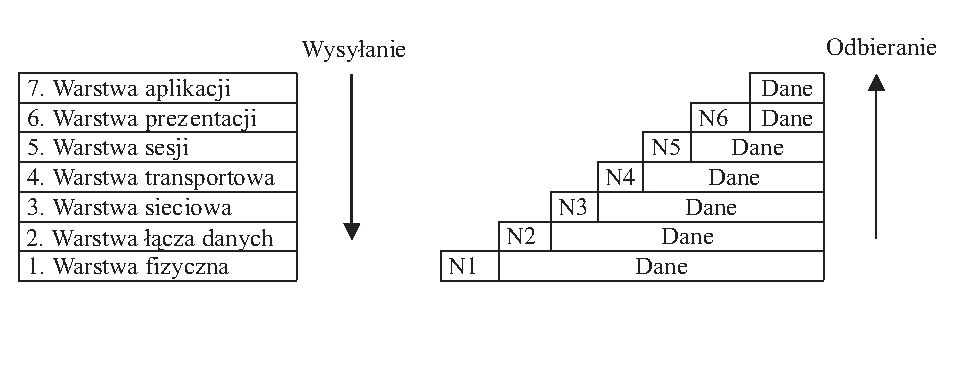
\includegraphics[width=5in]{./rysunki/nadawanie_i_odbieranie_naglowkow.eps}
\caption{Proces nadawania i odbierania nag��wk�w transmitowanym danym}
\label{nadawanie}
\end{figure}

Protoko�y poszczeg�lnych warstw zarz�dzaj� danymi w specyficzny dla siebie spos�b, mog� np. dokona� segmentacji, 
czyli podzia�u danych na mniejsze fragmenty przed przes�aniem ich do ni�szej warstwy. Ka�dy fragment otrzymuje 
wtedy odpowiedni nag��wek, kt�ry umo�liwia analogicznemu protoko�owi w komputerze adresata danych scalenie 
fragment�w podczas odbierania pakietu. Nag��wki umo�liwiaj� r�wnie� zarz�dzanie po��czeniami np. 
multipleksowanie po��cze� czyli wykorzystywanie jednego po��czenia, �ci�lej -- punktu dostarczania us�ug SAP 
(ang. \emph{Service Access Point})  warstwy ni�szej, np. sieciowej do obs�ugi kilku po��cze� nawi�zanych w warstwie 
bezpo�rednio wy�szej (tu transportowej). Odpowiednia informacja zawarta w nag��wku warstwy wy�szej umo�liwia 
wtedy identyfikacj� odbiorcy danych. Model ISO/OSI definiuje dwa tryby komunikacji. Komunikacje po��czeniow� 
stosuje si� gdy kluczowym wymaganiem jest niezawodno�� transmisji, musi by� wtedy znany zar�wno odbiorca jak i 
nadawca danych, a odbiorca potwierdza dotarcie do niego ka�dego fragmentu pakietu lub sygnalizuje konieczno�� 
retransmisji w przypadku b��du. Komunikacja bezpo��czeniowa nie zapewnia niezawodno�ci, dane wysy�a si� bez 
oczekiwania na potwierdzenie, a nadawca  i odbiorca nie s� znani, chyba �e wynika to z zawarto�ci pakietu, 
pakiety wysy�ane w trybie bezpo��czeniowym nazywamy datagramami.

W praktyce nie istnieje rozwi�zanie przemys�owe, kt�re �ci�le implementowa�oby wszystkie warstwy modelu ISO/OSI, 
cz�st� praktyk� jest np. ��czenie warstw fizycznej i ��cza danych w jedn� warstw�. R�wnie� protoko�y TCP/IP nie 
s� w pe�ni kompatybilne z modelem ISO/OSI, nie s� te� jednak ca�kowicie niekompatybilne. Wzajemn� relacj� 
architektury ISO/OSI i TCP/IP przedstawia poni�szy rysunek \cite{barylo1}.
\begin{figure}[h]
\centering
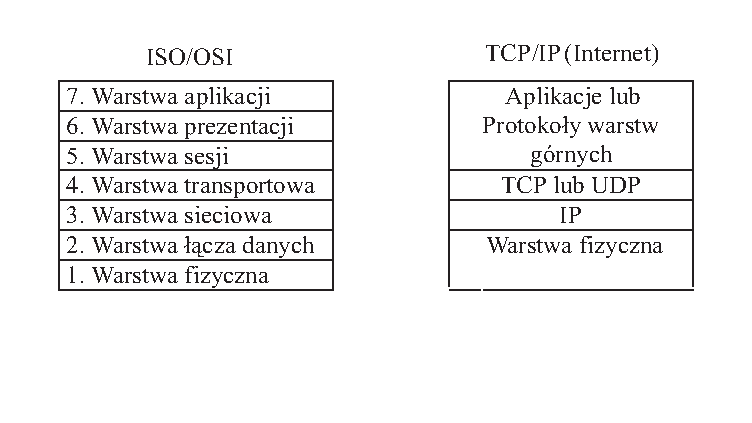
\includegraphics[width=5in]{./rysunki/architektura_ISO_a_tcp.eps}
\caption{Architektura ISO/OSI a TCP/IP}
\label{ISO_TCP}
\end{figure}
\section{Protok� IP}

Protok� IP (ang. \emph{Internet Protocol}) dzia�a w warstwie sieciowej i jest podstawowym protoko�em rodziny TCP/IP --
wszystkie dane nap�ywaj�ce z wy�szych warstw przesy�ane s� w sieci jako datagramy IP. Protok� ten �wiadczy 
zawodne, bezpo��czeniowe us�ugi dostarczania pakiet�w. Przez zawodne rozumiemy tu tak� w�a�ciwo��, �e IP nie 
daje gwarancji dostarczenia pakietu do punktu przeznaczenia, a wszelkie mechanizmy zapewnienia niezawodno�ci transmisji musz�
zosta� zapewnione przez protoko�y wy�szych warstw (np. TCP). Termin bezpo��czeniowy oznacza tu, �e IP nie 
przechowuje �adnej informacji na temat prawid�owo przesy�anych datagram�w, ka�dy z nich obs�ugiwany jest osobno, 
co w praktyce mo�e oznacza�, �e datagramy mog� dociera� do adresata w innej kolejno�ci, ni� zosta�y wys�ane. 
Wszystkie dane konieczne do poprawnej pracy IP zawarte s� w jego nag��wku, kt�ry typowo (je�li nie zawiera 
opcji) ma d�ugo�� 20 bajt�w i przedstawiony poni�ej format \cite{barylo2}.

\begin{figure}[h]
\centering
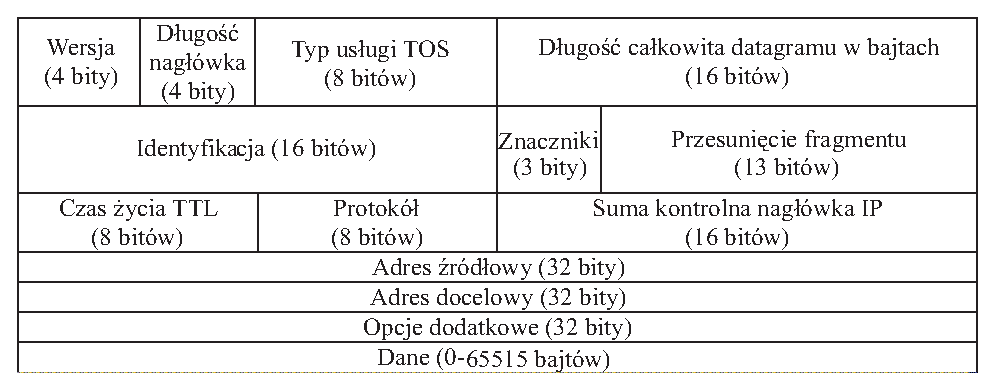
\includegraphics[width=5in]{./rysunki/datagram_ip.eps}
\caption{Format datagramu IP z wyr�nieniem nag��wka}
\label{datagram_ip}
\end{figure}

Pole \emph{d�ugo�� nag��wka} okre�la d�ugo�� nag��wka w 32--bitowych s�owach i wraz z polem D�ugo�� ca�kowita datagramu 
s�u�y do okre�lenia miejsca w kt�rym zaczynaj� si� w�a�ciwe dane. Ca�kowita d�ugo�� datagramu ograniczona jest 
zwykle przez warstw� fizyczn� np. dla sieci Ethernet jest to maksymalnie 1500 bajt�w a wielko�� t� nazywamy MTU 
(ang. \emph{Maximum Transmission Unit}) danej sieci.

Pole \emph{identyfikacja} zawiera unikalny numer dla ka�dego wysy�anego datagramu. Je�eli przechodz�c przez kolejne 
w�z�y sieci datagram musi zosta� podzielony, to warto�� ta jest kopiowana do wszystkich nag��wk�w IP 
powstaj�cych fragment�w i wraz z warto�ci� pola Przesuni�cie fragmentu umo�liwia poprawne scalenie datagramu w 
punkcie docelowym. Pomocne s� w tym r�wnie� warto�ci bit�w pola Znaczniki. Ustawienie jednego z nich wskazuje, 
�e istnieje kilka fragment�w datagramu, ustawienie drugiego zabrania fragmentacji datagramu.

Pole \emph{czas �ycia TTL} wyznacza  maksymaln� liczb� router�w przez kt�re mo�e przej�� datagram (routerem 
nazywamy tu specjalizowane urz�dzenie lub odpowiednio oprogramowany komputer s�u��ce do przekazywania datagram�w 
pomi�dzy sieciami r�ni�cymi si� w warstwie fizycznej np. Ethernet i Token Ring, lecz pracuj�cymi w oparciu o 
wsp�lny protok� warstwy sieciowej - IP). Warto�� tego pola jest wielko�ci� ca�kowit� zmniejszan� o jeden przez 
ka�dy router, do kt�rego dociera datagram. Datagram z warto�ci� TTL r�wn� 0 usuwany jest z sieci, co zapobiega 
kr��eniu w niej b��dnie zaadresowanych datagram�w.

Pole \emph{protok�} okre�la typ protoko�u b�d�cego nadawc� datagramu i jednocze�nie protok� kt�ry powinien 
odebra� datagram w punkcie docelowym.

Kluczowe znaczenie dla wyznaczania trasy przesy�ania datagramu maj� pola \emph{adres docelowy} i \emph{adres �r�d�owy}. Na 
podstawie warto�ci pola Adres docelowy protok� IP dynamicznie wyznacza kolejny w�ze� sieci na drodze pakietu, 
proces ten nazywamy marszrutowaniem IP. Adres IP jest 32--bitowym numerem, kt�ry w spos�b unikalny wyznacza 
miejsce pod��czenia interfejsu sieciowego (karty sieciowej) do sieci. W adresie IP wyr�niamy cz�� globaln� 
okre�laj�c� adres sieci i cz�� lokaln� identyfikuj�c� komputer w konkretnej sieci. Istnieje pi�� klas adres�w IP (Rys.: \ref{klasy_ip}):
\begin{figure}[h]
\centering
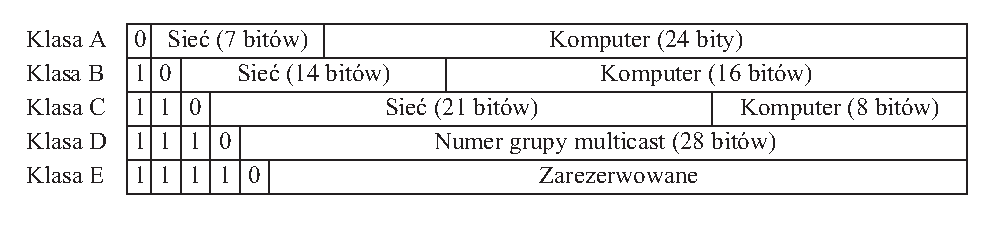
\includegraphics[width=5in]{./rysunki/klasy_adresow.eps}
\caption{Klasy adres�w IP}
\label{klasy_ip}
\end{figure}

Aby zapewni� unikalno�� adres�w sieci przydzielane s� one centralnie przez organizacj� InterNIC. Adres zapisuje
si� zwykle w tzw. notacji kropkowo -- dziesi�tnej, dzieli si� go na cztery o�miobitowe  grupy i warto�� ka�dej z 
nich zapisuje dziesi�tnie np.156.17.130.10 jest adresem serwera pocztowego Instytutu Sterowania i Techniki System�w
Politechniki Wroc�awskiej.

Istniej� trzy typy adres�w IP: adres unicast dotyczy pojedynczego komputera, adres broadcast dotyczy 
wszystkich komputer�w w danej sieci a adres multicast obejmuje grup� komputer�w nale��cych do jednej grupy 
multicastowej. Obecnie wszystkie implementacje IP musz� obs�ugiwa� tzw. adresowanie podsieci. Zamiast traktowa� 
adres IP jako proste z�o�enie adresu sieci i hosta (komputera) w cz�ci adresu wskazuj�cej hosta wydziela si� 
adres podsieci i w�a�ciwy adres hosta. Wynika to z faktu, �e adresy klasy A i B przeznaczaj� zbyt wiele bit�w na 
adres hosta, adres klasy B umo�liwia np. zaadresowanie 65535 komputer�w, a rzadko spotyka si� tak wiele host�w 
pod��czonych do jednej sieci. Podzia� 16 bitowego adresu hosta klasy B na dwie cz�ci o�miobitowe umo�liwia 
utworzenie w jednej sieci 255 podsieci z 254 hostami w ka�dej z nich. Decyzj� o podziale na podsieci podejmuje 
lokalny administrator, a informacj� o tym jaka ilo�� bit�w przeznaczona jest na adres podsieci przechowywana 
jest przez tzw. mask� podsieci. Jest to warto�� 32--bitowa  zawieraj�ca jedynki dla cz�ci adresuj�cej sie� i 
podsie� oraz zera dla cz�ci adresuj�cej hosta. Maska podsieci ma w om�wionym przypadku posta� 255.255.255.224.

Istnieje kilka zarezerwowanych adres�w IP wykorzystywanych do cel�w specjalnych. Obowi�zkowym adresem 
specjalnym jest adres interfejsu p�tli zwrotnej (ang. \emph{loopback}). Wi�kszo�� system�w przypisuje temu interfejsowi 
z definicji adres 127.0.0.1, cho� poprawny jest dowolny adres klasy A z adresem sieci 127. Datagramy kierowane 
na adres p�tli zwrotnej przechodz� przez warstw� transportow� i sieciow� po czym s� zawracane w g�r� stosu 
TCP/IP. Najcz�stszym zastosowaniem p�tli zwrotnej jest testowanie poprawno�ci dzia�ania protoko��w TCP/IP. 
Niekt�re systemy (np. system AIX) umo�liwiaj� dodawanie alias�w (dodatkowych adres�w) do adresu interfejsu p�tli 
zwrotnej.

Ka�dy komputer (host) pod��czony do sieci IP posiada co najmniej jeden adres IP, hosty posiadaj�ce kilka 
interfejs�w sieciowych posiadaj� po jednym adresie dla ka�dego interfejsu. Wszystkie te adresy, wraz z adresami 
specjalnymi i adresami typu broadcast przechowywane s� w tzw. tablicy marszrutowania (routingu). Protok� IP po otrzymaniu 
datagramu sprawdza, czy jego adres IP zgodny jest z kt�rym� z adres�w hosta lub jednym z adres�w specjalnych. 
Je�li tak jest datagram zostaje zaakceptowany. Post�powanie w przeciwnym wypadku zale�y od tego, czy warstwa IP 
skonfigurowana jest jako router. Je�eli host nie jest routerem nast�puje odrzucenie datagramu, w przeciwnym wypadku
uruchamiany jest opisany poni�ej algorytm marszrutowania.

Marszrutowanie IP dokonywane jest na podstawie kolejnych przej�� pomi�dzy w�z�ami sieci zapisanych (wraz z 
adresami w�asnymi hosta) w tablicy marszrutowania. Pojedynczy rekord tablicy routingu zawiera znany adres 
docelowy IP i adres IP na kt�ry nale�y skierowa� datagram je�li jego adres docelowy jest zgodny z adresem 
zapisanym w rekordzie. Je�eli nadawca i odbiorca s� bezpo�rednio po��czeni rekord tablicy marszrutowania zawiera 
wskazanie (w postaci adresu IP) na adresata datagramu, o czym informuje specjalny znacznik w danym rekordzie. 
W przeciwnym wypadku jest to adres routera stanowi�cego po��czenie z inn� sieci� lokaln� lub punkt wyj�cia do 
sieci rozleg�ej. Zak�ada si� �e router taki znajduje si� bli�ej punktu docelowego datagramu, gdy� IP nie zna 
pe�nej trasy dla �adnego z datagram�w adresowanych poza sie� lokaln�. Wyb�r drogi datagramu przebiega 
nast�puj�co \cite{barylo2}: 
w pierwszej kolejno�ci poszukiwany jest rekord zawieraj�cy w pe�ni zgodny adres docelowy IP. Je�li zostanie on 
znaleziony, datagram jest wysy�any na adres wskazany przez rekord. Mo�e by� to adres docelowy lub znane 
przej�cie przez router do innej sieci lokalnej.
Nast�pnie w tablicy marszrutowania  poszukiwany jest rekord z adresem sieci zgodnym z adresem sieci 
marszroutowanego datagramu. Je�li poszukiwania zako�cz� si� sukcesem datagram jest wysy�any na zawarty tam adres. 
W ten spos�b mog� by� obs�ugiwane  datagramy zaadresowane do host�w po��czonych z nadawc� przez wsp�ln� sie� 
(w sensie zgodno�ci adres�w globalnych IP). 
W przypadku niepowodzenia poprzednich poszukiwa� datagram wysy�any jest na adres IP routera domy�lnego.

Ostatni� czynno�ci� dokonywan� zanim datagram rzeczywi�cie opu�ci komputer nadawcy jest ustalenie jego adresu 
fizycznego w danej sieci lokalnej (np. adresu Ethernet lub Token Ring). Ka�de urz�dzenie: komputer, router, czy 
most (bridge) posiada unikalny w obszarze danej sieci lokalnej adres fizyczny. Odwzorowanie adresu IP w adres fizyczny 
dokonuje si� przy u�yciu protoko�u ARP (ang. \emph{Address Resolution Protocol}), opis jego dzia�ania le�y poza 
zakresem tej pracy.
Wypada zaznaczy�, �e adresy IP klasy B wyczerpa�y si� w roku 1997, co wymusi�o wprowadzenie nowej specyfikacji
protoko�u IP tzw. IPv6, kt�ry wprowadza adresy 128 bitowe. 

\section{Protok� TCP}

Protok� TCP (ang. \emph{Transmission Control Protocol}) zapewnia niezawodne, zorientowane 
po��czeniowo, oparte na strumieniach bajt�w (tzn. nie stosuj�ce �adnego arbitralnego podzia�u przesy�anych 
danych na jednostki sta�ej d�ugo�ci) us�ugi warstwy transportowej. Przed rozpocz�ciem transmisji dwie aplikacje 
u�ywaj�ce TCP musz� ustanowi� po��czenie w postaci wirtualnego kana�u transmisyjnego. Niezawodno�� tego 
po��czenia zapewniana jest przez dzia�ania takie jak: podzia� przesy�anych danych na segmenty o rozmiarze 
optymalnym ze wzgl�du na poprawno�� transmisji; utrzymywanie dla ka�dego segmentu osobnego zestawu zegar�w 
wyznaczaj�cych m. in. maksymalny czas oczekiwania na potwierdzenie odbioru segmentu i wymuszaj�cego retransmisj� 
w przypadku przekroczenia tego czasu; u�ywanie obowi�zkowych sum kontrolnych; odrzucanie zdublowanych 
datagram�w IP; zdolno�� rozpoznania kolejno�ci datagram�w IP (mog� one dociera� w kolejno�ci innej ni� by�y 
wysy�ane).

Informacj� kontroln� segmentu TCP zawiera przedstawiony poni�ej nag��wek \cite{barylo2}.
\begin{figure}[h]
\centering
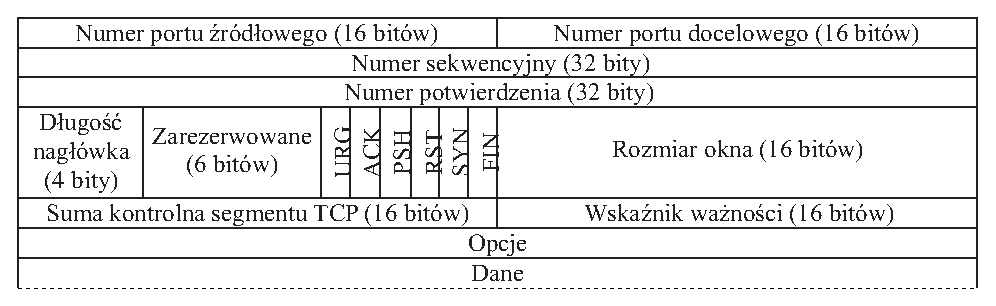
\includegraphics[width=5in]{./rysunki/format_segmentu_tcp.eps}
\caption{Format segmentu TCP z wyr�nieniem nag��wka.}
\label{segment_TCP}
\end{figure}

Pola \emph{numer portu �r�d�owego} i \emph{numer portu docelowego} zawieraj� wielko�ci ca�kowite i pe�ni� kluczow� rol� w 
identyfikacji po��cze� TCP. Numery port�w od 1 do 1023 s� zarezerwowane dla tzw. us�ug dobrze znanych i 
zazwyczaj przydzielane s� aplikacjom pracuj�cym jako serwery. Przyk�adowo serwery WWW (protok� HTTP) otrzymuj� 
numer portu 80, serwery FTP wykorzystuj� porty 20 i 21 a serwery pocztowe (SMTP) port 25. Do nawi�zania 
po��czenia proces klienta (np. przegl�darka WWW) uzyskuje od protoko�u TCP tzw. numer kr�tkotrwa�y unikalny dla 
ka�dej aplikacji u�ywaj�cej TCP w danym ho�cie. W przypadku przegl�darki WWW mo�e by� to numer 80 lub dowolny 
numer z zakresu 1024... 5000. Para port �r�d�owy -- port docelowy jest wystarczaj�ca do identyfikacji po��czenia 
po stronie klienta. Je�li nawet u�ytkownik uruchomi dwie identyczne aplikacje (np. dwie przegl�darki WWW), to 
otrzymaj� one r�ne numery kr�tkotrwa�e. Po stronie serwera sytuacja jest trudniejsza, typowo serwer poprzez 
multipleksacj� portu obs�uguje wiele po��cze� z u�yciem jednego numeru portu �r�d�owego (np. 80 dla serwera WWW),
mo�e si� wi�c zdarzy�, �e dw�ch niezale�nych klient�w zg�osi ten sam numer kr�tkotrwa�y portu docelowego. Do 
jednoznacznej identyfikacji po��cze� wykorzystuje si� kombinacj� numeru portu i adresu IP nazywan� gniazdem. 
Gniazda s� jednym z podstawowych poj�� interfejsu programisty TCP/IP.

Jak ju� wspomniano TCP przesy�a dane w postaci strumienia bajt�w, w praktyce oznacza to, �e wysy�any 
segment danych mo�e mie� ka�dorazowo inn�  d�ugo��. Do umo�liwienia uformowania z segment�w oryginalnego pakietu 
s�u�y warto�� pola \emph{numer sekwencyjny}. Je�li rozpatrzymy strumie� bajt�w przesy�any tylko w jedn� stron�, to 
warto�� tego pola okre�la  numer jaki ma w strumieniu ostatni bajt segmentu. Warto�� pocz�tkow� numeru 
sekwencyjnego ustala nadawca w momencie ustanawiania po��czenia. Je�li pocz�tkowym numerem sekwencyjnym by�o 
100, a pierwszy segment ma d�ugo�� 1024 bajty, to jego numerem sekwencyjnym jest 1123. Pierwszy bajt kolejnego 
segmentu sk�adaj�cego si� na pakiet b�dzie mia� numer 1124, je�li segment ten ma d�ugo�� 125 bajt�w, to jego 
numerem sekwencyjnym jest 1248. Koniec strumienia oznacza si� przez ustawienie flagi bitowej FIN w nag��wku 
ostatniego segmentu.

TCP wymaga potwierdze� odbioru ka�dego przes�anego segmentu. S�u�y do tego pole \emph{numer potwierdzenia}. Je�li 
zn�w rozpatrywa� przesy�anie danych w jedn� tylko stron�, to po odebraniu segmentu o numerze sekwencyjnym 1123 
klient wysy�a (pozbawiony danych) segment TCP z ustawion� flag� bitow� ACK i warto�ci� numeru potwierdzenia 1124 
(jest to numer kolejny oczekiwanego bajtu). Aby zapewni� niezale�ne przesy�anie danych w obydwu kierunkach, 
ka�da ze stron pami�ta numery sekwencyjne wymienianych segment�w. Opisany powy�ej segment potwierdzenia posiada 
wi�c ustalany przez jego nadawc� numer sekwencyjny (np. 136), kt�ry serwer musi potwierdzi� ustawiaj�c flag� ACK 
i umieszczaj�c w polu Numer sekwencyjny odpowiedni� warto�� (tutaj 137). Konsekwencj� takiej strategii wymiany 
potwierdze� jest fakt, �e w trakcie wymiany danych flaga ACK jest ci�gle ustawiona (ma warto�� logiczn� 1).
Pole D�ugo�� nag��wka zawiera liczb� 32--bitowych s��w sk�adaj�cych si� na nag��wek, nast�puje po nim 6 
zarezerwowanych bit�w i kolejno 6 flag bitowych. Istotn� flag� jest SYN, kt�ra jest ustawiona podczas wymiany 
segment�w nawi�zuj�cych po��czenie i ustalania pocz�tkowych numer�w sekwencyjnych. 

Pole \emph{rozmiar okna} zawiera warto�� ca�kowit�, przy pomocy kt�rej odbiorca deklaruje jak� ilo�� bajt�w 
nadawca mo�e wys�a� bez oczekiwania na potwierdzenie (inaczej -- jak� ilo�� bajt�w odbiorca jest w stanie przyj�� 
jednorazowo). Pole ma zastosowanie w przypadku transmisji wg tzw. protoko�u przesuwnego okna, a jego warto�� 
mo�e si� zmienia� w trakcie  transmisji.

Wa�n� rol� w trakcie nawi�zywania po��czenia pe�ni pole \emph{opcje}. W polu tym uczestnicy po��czenia wymieniaj� 
si� informacj� jak du�y jest pojedynczy segment, kt�ry s� w stanie przyj��. Ustalone w ten spos�b maksymalne 
wielko�ci segmentu MSS (ang. \emph{Maximum Segment Size}) pozostaj� sta�e dla obydwu ko�c�wek po��czenia przez ca�y 
czas jego trwania. 

Warto�� t� ustala si� z uwzgl�dnieniem nak�adanego przez warstw� fizyczn� ograniczenia na maksymalny rozmiar 
datagramu IP (MTU).

Aby m�c zarz�dza� po��czeniami oprogramowanie protoko�u TCP utrzymuje tablic� po��cze�. Pojedynczy rekord takiej 
tablicy opisuje jedno po��czenie i zawiera pola: 
\begin{itemize}
\item Status (zamkni�te, w trakcie zamykania, oczekiwanie na potwierdzenie itp.)
\item Adres lokalny -- adres IP hosta �r�d�owego (przechowuj�cego tablic�)
\item Port lokalny -- numer portu hosta �r�d�owego
\item Adres zdalny -- adres IP hosta docelowego
\item Port zdalny -- numer portu docelowego
\end{itemize}

Protok� TCP wykorzystywany jest przez wiele protoko��w wy�szych warstw, dla kt�rych najistotniejsz� spraw� jest 
zapewnienie niezawodno�ci transmisji. TCP u�ywaj� m. in. HTTP, FTP czy SMTP, kt�re zostan� kr�tko om�wione w 
dalszej cz�ci tej pracy. System DNS korzysta z protoko�u TCP podczas wymiany danych pomi�dzy serwerami DNS w 
trakcie uaktualniania ich tablic odwzorowa�.

\section{Protok� UDP}

Protok� UDP (ang. \emph{User Datagram Protocol}) jest prostym, bezpo��czeniowym protoko�em warstwy transportowej 
wykorzystuj�cym datagramy. Z ka�dego pakietu danych skierowanego do UDP przez warstwy g�rne formowany jest 
jeden datagram UDP, z kt�rego (inaczej ni� w przypadku TCP) tworzony jest dok�adnie jeden datagram IP. Aplikacja 
wysy�aj�ca pakiet musi sama zadba� o to, by jego d�ugo�� nie przekroczy�a MTU. UDP (w przeciwie�stwie do TCP) 
nie implementuje �adnych mechanizm�w zapewniaj�cych niezawodno�� transmisji.  Nag��wek datagramu UDP ma bardzo 
prosty format \cite{barylo2}.
\begin{figure}[h]
\centering
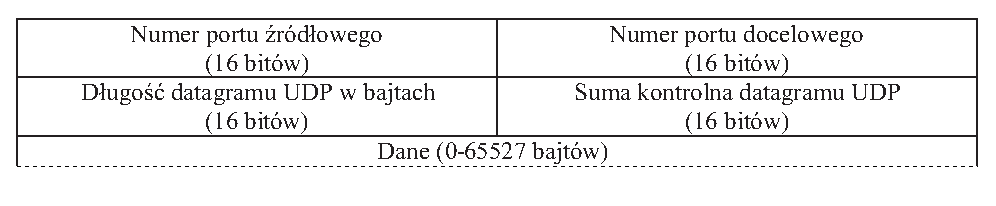
\includegraphics[width=5in]{./rysunki/datagram_udp.eps}
\caption{Datagram UDP z wyr�nionym nag��wkiem.}
\label{datagram_udp}
\end{figure}
 
\section{Protok� FTP}

Protok� FTP (ang. \emph{File Transfer Protocol}) jest standardowym w Internecie protoko�em przesy�ania dowolnego 
rodzaju plik�w. Jest to protok� warstw wy�szych, i przez to jest cz�sto b��dnie uto�samiany z aplikacjami 
klienta FTP. FTP korzysta w warstwie transportowej z us�ug protoko�u TCP. Do obs�ugi transmisji FTP, w 
przeciwie�stwie do wi�kszo�ci protoko��w, otwiera a� dwa po��czenia TCP : po��czenie steruj�ce o numerze portu 
docelowego 21 i po��czenie transmisji danych o numerze portu 20. Przez po��czenie steruj�ce aplikacje FTP 
wymieniaj� zdefiniowane w protokole polecenia i potwierdzenia. Po��czenie transmisji u�ywane jest do binarnego 
przesy�ania danych. Schemat obs�ugi po��czenia przez procesy klienta i serwera FTP przedstawia rysunek \ref{polaczenie_ftp}.
\begin{figure}[h]
\centering
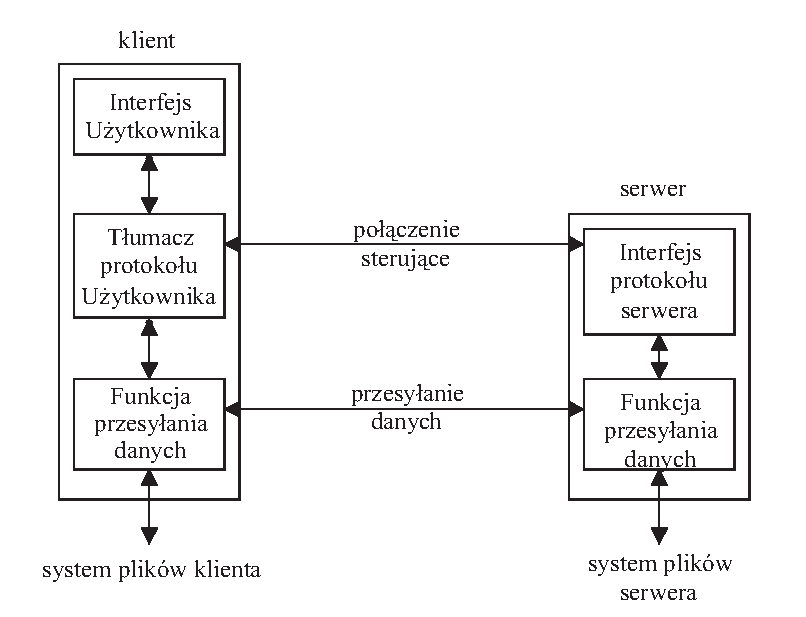
\includegraphics[width=5in]{./rysunki/obsluga_ftp.eps}
\caption{Obs�uga po��czenia ftp.}
\label{polaczenie_ftp}
\end{figure}

Po��czenie przesy�ania danych nawi�zywane jest dla ka�dego przesy�anego pliku. FTP mo�e przesy�a� pliki w 
jednym z trzech tryb�w: jako strumie� bajt�w, jako seri� blok�w podzielonych nag��wkami lub w rzadko stosowanym 
trybie z kompresj� FTP (kompresji podlegaj� tylko ci�gi zerowych bajt�w). FTP rozpoznaje formaty ASCII i EBCDIC 
-- przesy�ane s� one w postaci rekord�w o sta�ej d�ugo�ci, pozosta�e pliki traktowane s� jako pliki binarne i 
przesy�ane jako strumie� bajt�w.

Polecenia FTP wymieniane przez po��czenie steruj�ce maj� posta� ci�g�w wielkich liter ASCII o d�ugo�ci 3 
lub 4 bajt�w. Ka�de nawi�zanie po��czenia z serwerem FTP wymaga podania nazwy u�ytkownika i has�a, jest to 
prosty mechanizm zapewniaj�cy kontrol� dost�pu do zasob�w serwera. O tym, jakie pliki udost�pnia� konkretnym 
u�ytkownikom decyduje administrator serwera FTP.
Wed�ug bada� prowadzonych w szkieletowej sieci NSFNET dane FTP stale stanowi� ok. 20\% pakiet�w 
transmitowanych w tej sieci. 

\section{Protok� SNMP}

Protok� SNMP (ang. \emph{Simple Network Management Protocol}) pierwotnie zaprojektowano jako uniwersalne narz�dzie, 
kt�re umo�liwi zdalne nadzorowanie �luz (ang. \emph{gateway})  i router�w w sieciach rozleg�ych. W miar� jego rozwoju 
protok� uzupe�niono o mo�liwo�� zarz�dzania wszelkim typem urz�dze� sieciowych w sieciach TCP/IP. SNMP ka�dej 
sieci opiera si� o trzy sk�adniki:
\begin{itemize}
\item MIB (ang. \emph{Management Information Base}) jest to baza danych opisuj�ca stan danego urz�dzenia;
\item SMI (ang. \emph{Structure and Identification of Management Information}) jest zestawem powszechnie stosowanych 
schemat�w s�u��cych odwo�ywaniu si� do zmiennych MIB;
\item SNMP okre�la zasady komunikowania si� pomi�dzy aplikacj� zarz�dzaj�c� sieci� (serwerem SNMP), a procesem 
steruj�cym urz�dzeniem (agentem).
\end{itemize}

Ka�dy element sieci, kt�ry ma by� zarz�dzany przez SNMP, musi przechowywa� informacj� o parametrach okre�laj�cych
stan danego elementu, a maj�cych wp�yw na prac� sieci. Baza danych zawieraj�ca te parametry to w�a�nie MIB. W 
przypadku urz�dzenia takiego jak router rekord MIB mo�e np. zawiera� informacj� o stopniu zape�nienia jego 
bufor�w pami�ci. MIB nie musi dotyczy� element�w �ci�le sprz�towych istniej� np. MIB system�w operacyjnych. 
Spos�b odwo�ywania si� do element�w MIB okre�laj� schematy SMI.

W ka�dej sieci, kt�rej elementy zarz�dzane s� wed�ug standard�w SNMP istnieje wydzielony host, na kt�rym 
pracuje specjalistyczna aplikacja (serwer SNMP) s�u��ca monitorowaniu i zarz�dzaniu prac� sieci. Proces, kt�ry 
dzia�a w zarz�dzanym elemencie i  aktualizuje MIB oraz udost�pnia serwerowi jej zmienne lub ustawia je na zadane 
przez serwer warto�ci nazywany jest agentem SNMP.

W celu umo�liwienia komunikacji pomi�dzy serwerem a agentami SNMP definiuje pi�� typ�w komunikat�w. Trzy 
z nich wysy�ane s� zawsze w kierunku serwer--klient i s�u�� pobieraniu lub ustawianiu zmiennych MIB. Dwa typy 
komunikat�w wysy�ane s� w kierunku klient--serwer. Jeden z nich zwraca ��dan� lub nowo ustawion� warto�� 
zmiennej MIB, drugi jest komunikatem alarmowym wysy�anym przez agenta w przypadku b��dnej pracy urz�dzenia lub 
przekroczenia krytycznej warto�ci przez kt�r�� ze zmiennych MIB.
Serwer SNMP musi utrzymywa� w miar� aktualn� informacj� o stanie sieci, dlatego agenci SNMP przepytywani 
s� w regularnych odst�pach czasu, posiadaj�c jednocze�nie mo�liwo�� raportowania o sytuacjach awaryjnych. Fakt, 
�e cztery z pi�ciu mo�liwych rodzaj�w komunikacji pomi�dzy serwerem a agentem SNMP to pary typu pojedyncze 
pytanie--pojedyncza odpowied� (wyj�tek stanowi� komunikaty alarmowe) oraz ch�� minimalizacji obci��enia sieci 
powodowanego przez pakiety s�u��ce jej zarz�dzaniu spowodowa�y, �e SNMP w warstwie transportowej korzysta z 
us�ug UDP. Zawodno�� tego protoko�u sprawia, �e serwery SNMP powinny (szczeg�lnie w sytuacjach awaryjnych) 
stosowa� mechanizmy odmierzania czasu na odpowied� agenta i ewentualnej retransmisji komunikat�w. Warto doda�, 
�e SNMP nie jest zale�ny w warstwie sieciowej od IP, przy odpowiedniej konfiguracji rol� protoko�u sieciowego 
mo�e spe�nia� np. IPX/SPX.

\section{Protok� SMTP}

Protok� SMTP (ang. \emph{Simple Mail Transfer Protocol}) jest prostym protoko�em warstw g�rnych wykorzystywanym do 
przesy�ania poczty elektronicznej w sieciach TCP/IP. W warstwie transportowej SMTP wykorzystuje protok� TCP i 
posiada przydzielony numer portu 25. Nale�y wyja�ni�, �e programy pocztowe, z kt�rymi kontaktuj� si� szeregowi 
u�ytkownicy Internetu stanowi� jedynie ko�cowe narz�dzia, w terminologii fachowej nazywane agentami u�ytkownika 
UA (ang. \emph{User Agent}) s�u��ce do pobierania list�w z elektronicznych skrzynek pocztowych lub umieszczania ich w 
kolejce do najbli�szego serwera pocztowego. Programy rzeczywi�cie zajmuj�ce si� przesy�aniem wiadomo�ci pomi�dzy 
serwerami pocztowymi nazywane s� agentami przesy�ania komunikat�w MTA (ang. \emph{Message Transfer Agent}). Przyk�adem 
MTA jest unixowy Sendmail. Protok� SMTP s�u�y w�a�nie do komunikacji pomi�dzy poszczeg�lnymi MTA. Schemat 
przesy�ania poczty w Internecie przedstawia poni�szy rysunek.
\begin{figure}[h]
\centering
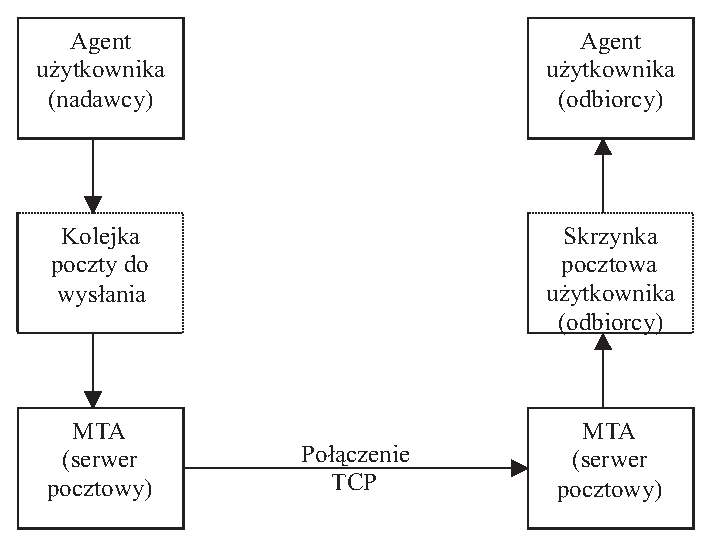
\includegraphics[width=5in]{./rysunki/obsluga_poczty.eps}
\caption{Schemat przesy�ania poczty elektronicznej}
\label{poczta}
\end{figure}

Komunikacja pomi�dzy MTA odbywa si� wed�ug modelu klient -- serwer, przy czym klientem nazywamy MTA, kt�ry inicjuje dane 
po��czenie. Po��czenie rozpoczyna si� od przes�ania danych identyfikuj�cych nadawc�, a w odpowiedzi nadchodzi pakiet 
identyfikuj�cy odbiorc�. Nast�pnie przesy�ana jest w�a�ciwa wiadomo�� i po��czenie jest zamykane. Do obs�ugi poczty 
elektronicznej SMTP definiuje tylko 13 polece� (dla por�wnania FTP posiada 40 polece�), kt�re s� czterobajtowymi ci�gami 
wielkich liter ASCII.

Wiadomo�� elektroniczna sk�ada si� w SMTP z trzech cz�ci. Koperty czyli danych pozwalaj�cych MTA zidentyfikowa� 
nadawc� i odbiorc� wiadomo�ci, nag��wk�w czyli danych wykorzystywanych przez agent�w u�ytkownika (np. data 
wys�ania wiadomo�ci) i w�a�ciwej wiadomo�ci.
Pakiety SMTP stanowi� od 8 do 13 procent pakiet�w transmitowanych w sieci szkieletowej NSFNET. 

\section{Protok� POP3.}

Opisany powy�ej protok� SMTP jest efektywnym narz�dziem umo�liwiaj�cym przesy�anie poczty elektronicznej 
pomi�dzy pracuj�cymi w spos�b ci�g�y serwerami SMTP. Aby pojedynczy u�ytkownik sieci m�g� odbiera� poczt� 
bezpo�rednio przez SMTP w jego stacji roboczej musia�by ci�gle dzia�a� proces typu MTA, co jest cz�sto 
niemo�liwe ze wzgl�d�w czysto technicznych. Rozwi�zanie tego problemu jest bardzo proste. W pod��czonych do 
Internetu sieciach lokalnych wydziela si� dzia�aj�cy non--stop  serwer pocztowy wraz z oprogramowaniem 
zachowuj�cym na dysku wiadomo�ci nadchodz�ce do u�ytkownik�w sieci. Protok� POP3 (ang. \emph{Post Office Protocol 
version 3}) umo�liwia dynamiczny dost�p do wiadomo�ci przechowywanych na takim wydzielonym serwerze \cite{barylo9}. Protok� ten 
korzysta z TCP i numeru portu 110. POP3 definiuje 13 polece� w postaci czterobajtowych ci�g�w ASCII. 

Po��czenie POP3 rozpoczyna si� od identyfikacji u�ytkownika i podania has�a nast�pnie serwer i klient wymieniaj� 
dane po czym sesja ko�czy si�.

Producenci aplikacji pocztowych (UA) stosuj� dwa protoko�y, SMTP do bezpo�redniego wysy�ania poczty i POP3 
do odbierania jej z serwera pocztowego.

Pakiety POP3 najcz�ciej spotka� mo�na w sieciach lokalnych, gdzie mog� stanowi� znaczny procent 
transmitowanych danych.

\section{Protok� SSL}

Protok� SSL (ang. \emph{Secure Socket Layer}) jest protoko�em rezyduj�cym bezpo�rednio nad protoko�em TCP i 
dostarczaj�cym dowolnemu protoko�owi wy�szych warstw (np. HTTP) przezroczyste us�ugi maj�ce zapewni� poufno�� 
przesy�anych danych. SSL wykorzystuje port TCP o numerze 443. Bezpiecze�stwo po��czenia oparte jest o trzy cechy 
protoko�u SSL: symetryczne szyfrowanie danych w oparciu o np. algorytmy DES lub RC4; autoryzacj� host�w z 
wykorzystaniem szyfrowania asymetrycznego lub z kluczem publicznym (RSA, DSS) i  kontrol� poprawno�ci transmisji 
poprzez zastosowanie szyfrowanych sum kontrolnych MAC (ang. \emph{Message Autenthication Codes}).

W protokole SSL wyr�niamy dwie warstwy: warstw� powitania i warstw� rekord�w. Warstwa powitania (ang. \emph{Handshake Layer}) 
inicjuje po��czenie 
pomi�dzy klientem a serwerem. Po wzajemnej identyfikacji host�w nast�puje faza negocjacji algorytm�w, kt�re b�d� 
u�yte do szyfrowania transmisji (wyb�r ten zale�y od mocy obliczeniowej host�w). Od momentu ustalenia sposobu 
kodowania wszystkie dane s� szyfrowane.

Warstwa rekord�w (ang. \emph{Record Layer}) rezyduje pomi�dzy warstw� powitania a TCP i jest odpowiedzialna za 
enkapsulacj� danych nap�ywaj�cych z wy�szych warstw do postaci rekord�w o maksymalnej d�ugo�ci 16384 bajt�w, 
szyfrowanie rekord�w oraz do��czanie MAC \cite{barylo10}.

Poniewa� SSL nie interpretuje nap�ywaj�cych do niego danych istnieje mo�liwo�� przesy�ania hipertekstu z 
u�yciem SSL. Tak skonfigurowany serwer WWW nazywamy serwerem HTTPS lub serwerem SSL. Szyfrowane s� w�wczas 
wszystkie elementy  transmisji tzn. zar�wno dokumenty jak i same polecenia HTTP, co wymaga odpowiedniej 
konfiguracji przegl�darki.

\section{URL i DNS}
	
U�ytkownik Intrenetu do identyfikacji zasob�w sieciowych stosuje zazwyczaj adres URL (ang. \emph{Uniform Resource 
Locator}). URL zapisujemy w postaci \cite{barylo5, barylo6}:\\
\emph{typ\_us�ugi://nazwa\_serwera.nazwa\_domeny/�cie�ka\_dost�pu/nazwa\_zasobu}. 
Na przyk�ad URL http://www.netscape.com/main.html jest wskazaniem na zapisany w postaci pliku HTML 
dokument hipertekstowy main.html znajduj�cy si� na �cie�ce dost�pu (mo�e by� to nazwa katalogu lub jej alias) 
News/Sport w serwerze home umieszczonym w domenie netscape.com. Dokument ten dost�pny jest poprzez protok� 
HTTP.

Cz�� URL okre�laj�ca typ us�ugi interpretowana jest przez aplikacj� u�ywan� do po��czenia z Internetem 
np. przegl�dark� WWW. �cie�ka dost�pu i nazwa zasobu przesy�ane s� do serwera i interpretowane przez jego system 
plik�w. Nazwa serwera i nazwa domeny s� tylko nazwami symbolicznymi i musz� by� zamienione na adres IP zanim 
zostanie nawi�zane po��czenie z serwerem. Zamiana ta mo�liwa jest dzi�ki systemowi DNS.

DNS (ang. \emph{Domain Name System}) jest rozproszon� baz� danych umieszczon� na wielu Internetowych hostach, 
kt�re nazywamy serwerami DNS. Ka�dy komputer, kt�ry chce korzysta� z DNS musi pami�ta� w swojej konfiguracji 
adres IP najbli�szego serwera DNS. Nazwa DNS mo�e mie� d�ugo�� do 63 znak�w. Przestrze� nazw DNS ma struktur� 
hierarchicznego, podzielonego na poziomy drzewa. M�wimy, �e domena wy�szego poziomu com zawiera domen� ni�szego 
poziomu netscape. Rysunek \ref{dns} przedstawia hierarchiczn� organizacj� DNS \cite{barylo3}.
\begin{figure}[h]
\centering
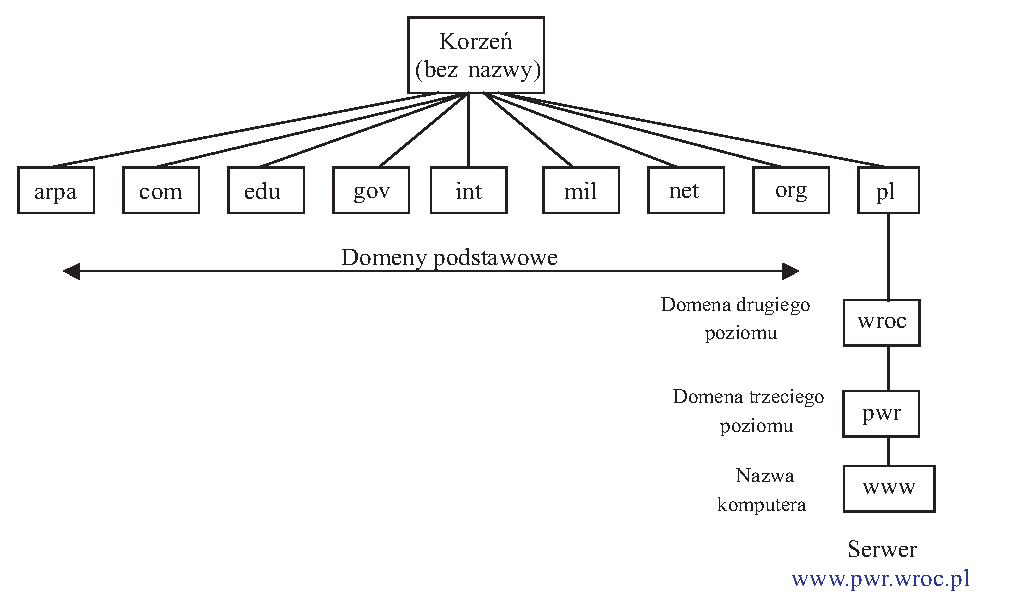
\includegraphics[width=5in]{./rysunki/struktura_dns.eps}
\caption{Hierarchiczna struktura DNS}
\label{dns}
\end{figure}
																
Domeny arpa, com, edu, gov, int, mil, net, org i domeny pa�stwowe takie jak pl nazywamy domenami podstawowymi. 
Obejmuj� one nast�puj�ce komputery: arpa -- sie� ARPANET; com -- organizacje komercyjne; edu -- instytucje edukacyjne; 
gov -- organizacje rz�dowe; int -- organizacje mi�dzynarodowe; mil -- armia USA; net -- sieci; org -- pozosta�e 
organizacje. Organizacje rz�dowe z kraj�w innych ni� USA grupowane mia�y by� w dwuliterowych domenach pa�stwowych
np. ae -- Zjednoczone Emiraty Arabskie; pl -- Polska; zw -- Zimbabwe. Obecnie podzia� ten nie jest �ci�le 
przestrzegany, wiele organizacji komercyjnych rejestruje si� w domenie podstawowej (np. empik.com), inne stosuj� 
podzia� w ramach domen pa�stwowych (np. creamsoft.com.pl). spotyka si� r�wnie� nazwy w og�le nie mieszcz�ce si� 
w opisanym schemacie np. www.rmf.fm.

Obszarem nazywamy oddzielnie administrowan� cz�� drzewa DNS. Typowym obszarem jest domena drugiego lub 
trzeciego poziomu  np. netscape.com lub pwr.wroc.pl. Je�li w domenie zarejestrowanych jest wiele komputer�w 
zwykle (dla zwi�kszenia efektywno�ci dzia�ania DNS) dzieli si� j� na kilka obszar�w.

W ka�dym obszarze musi znajdowa� si� podstawowy serwer DNS, kt�ry w specjalnym zestawie plik�w przechowuje 
odwzorowania wszystkich nazw komputer�w z danego obszaru w ich adresy IP. Drugoplanowe serwery DNS informacje o 
odwzorowaniach uzyskuj� z serwera podstawowego korzystaj�c z po��czenia TCP o numerze portu 53. Serwery 
drugoplanowe przechowuj� (na zasadzie pami�ci cache dla klient�w, kt�rzy zwracaj� si� do nich z zapytaniami) 
odwzorowania obejmuj�ce tylko cz�� obszaru i odwzorowania o kt�re klienci najcz�ciej pytaj�. W sta�ych 
odst�pach czasu (typowo co 3 godziny) serwery drugoplanowe DNS uaktualniaj� swe tablice odpytuj�c serwer 
podstawowy. Odwzorowanie nazwy spoza obszaru nie musi by� znane ani serwerowi podstawowemu, ani drugoplanowemu, 
chyba �e przechowywane jest w pami�ci cache (jest cz�sto poszukiwane). Je�li serwer podstawowy nie zna ��danego 
odwzorowania musi si� zwr�ci� z zapytaniem (z wykorzystaniem portu 53 TCP) do jednego z serwer�w g��wnych DNS 
(w 1993 roku by�o ich w Internecie 8), kt�rych obowi�zkiem jest wskazanie serwera DNS b�d�cego w stanie zwr�ci� 
poprawne odwzorowanie.

Proces odpowiedzialny za odwzorowanie nazw po stronie klienta nazywamy rezolwerem lub przelicznikiem nazw. 
Zwykle jest on zintegrowany z aplikacj� (np. przegl�dark� WWW) i na zasadzie pami�ci cache przechowuje lokalnie 
pewn� ilo�� odwzorowa�. Je�li wywo�ywana przez u�ytkownika nazwa nie jest znana lokalnie rezolwer korzystaj�c z 
portu UDP 53 wysy�a zapytanie do najbli�szego drugoplanowego serwera DNS. Je�li odpowied� nie przekracza 512 
bajt�w zwracana jest w postaci datagramu UDP, w przeciwnym wypadku jako datagram UDP wysy�ane jest pierwsze 512 
bajt�w i w nag��wku DNS ustawiana jest flaga informuj�ca o tym fakcie. Zazwyczaj rezolwer ponawia wtedy 
zapytanie korzystaj�c z portu 53 TCP, co umo�liwia przes�anie pe�nej odpowiedzi w jednym segmencie TCP. Rezolwer 
mo�e wys�a� dwa typy zapyta�: zapytanie rekurencyjne umo�liwia serwerowi DNS ,,konsultacje'' z serwerami wy�szego 
rz�du przed zwr�ceniem odpowiedzi; zapytanie iteracyjne wymaga od niego natychmiastowej odpowiedzi, kt�ra je�li 
dany serwer nie zna odwzorowania, musi mie� posta� adresu IP serwera DNS b�d�cego (wedle ,,wiedzy'' zapytanego 
serwera DNS) w stanie udzieli� poprawnej odpowiedzi. Ze wskazanym serwerem DNS resolwer komunikuje si� 
bezpo�rednio. Poniewa� istnieje mo�liwo��, �e  nieprawid�owe zapytanie rekurencyjne niesko�czenie b�dzie kr��y� 
pomi�dzy serwerami DNS w nag��wku DNS zdefiniowano pole ograniczaj�ce liczb� rekurencji. Warto�� tego pola 
zmniejszana jest o jeden przez ka�dy serwer DNS, kt�ry przetwarza zapytanie. Zapytanie z zerow� warto�ci� tego 
pola jest odrzucane i serwer komunikuje b��d. W takim wypadku rezolwer mo�e u�y� zapytania iteracyjnego, ponowi� 
zapytanie rekurencyjne ze zwi�kszon� warto�ci� pola ograniczaj�cego rekurencje lub zg�osi� u�ytkownikowi b��d 
DNS. Rysunki \ref{rekurencyjne} i \ref{iteracyjne} przedstawiaj� obs�ug� obydwu typ�w zapyta� \cite{barylo3}.
\begin{figure}[h]
\centering
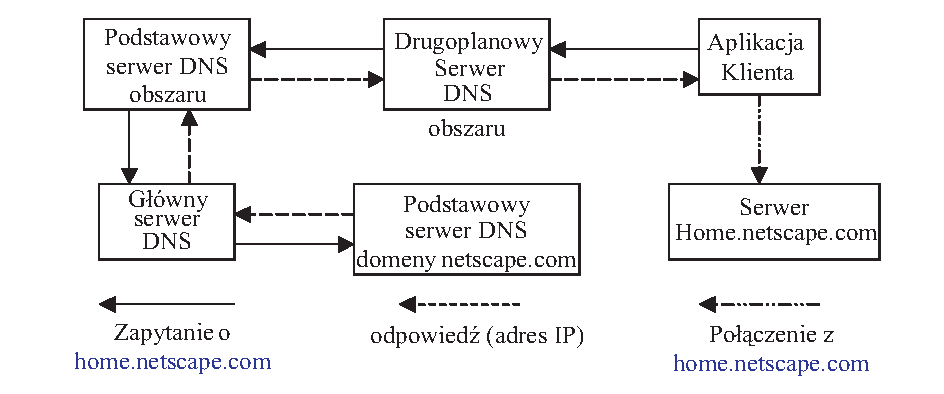
\includegraphics[width=4in]{./rysunki/zapytanie_rekurencyjne.eps}
\caption{Obs�uga zapytania rekurencyjnego}
\label{rekurencyjne}
\end{figure}

\begin{figure}[h]
\centering
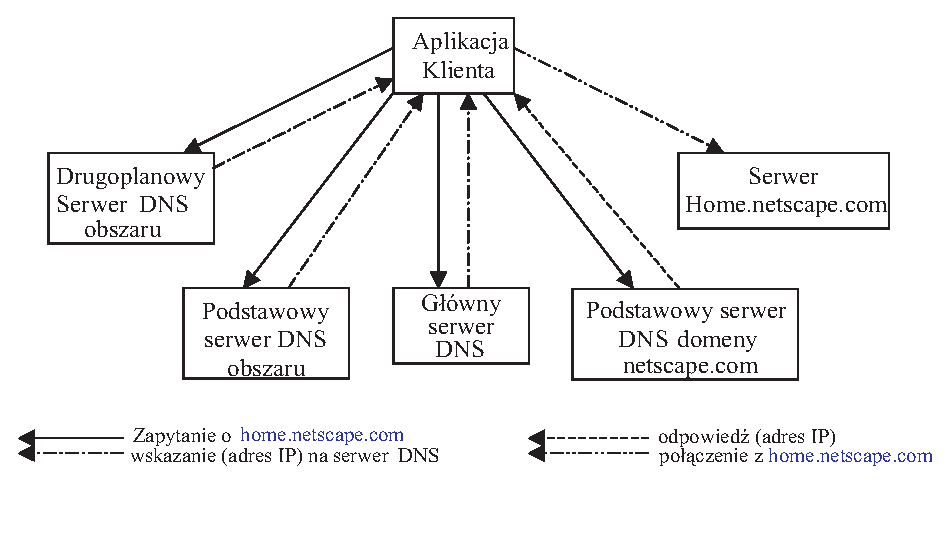
\includegraphics[width=4in]{./rysunki/zapytanie_iteracyjne.eps}
\caption{Obs�uga zapytania iteracyjnego}
\label{iteracyjne}
\end{figure}

Powy�sze rysunki przedstawiaj� ,,najgorszy'' przypadek, gdy adres IP serwera www.netscape.com znany jest dopiero 
przez podstawowy serwer DNS domeny (obszaru) netscape.com. W rzeczywisto�ci istnieje du�e prawdopodobie�stwo, �e 
odwzorowanie nazwy przechowywane jest przez pami�� cache jednego z bli�szych klientowi serwer�w.
Informacje o wzajemnych odwzorowaniach nazw w adresy IP serwery DNS przechowuj� w postaci rekord�w zasob�w 
DNS--DNS RR (ang. \emph{DNS Resource Record}). Rekordy te przesy�ane s� do aplikacji klienta jako odpowied� na 
zapytanie. Pojedynczy DNS RR ma przedstawion� na rys. \ref{dns_rr} struktur� \cite{barylo3}.
\begin{figure}[h]
\centering
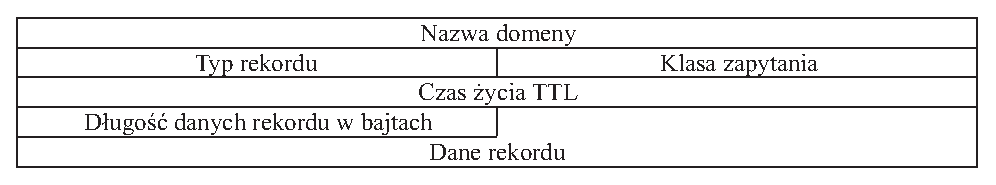
\includegraphics[width=5in]{./rysunki/format_dns_rr.eps}
\caption{Format DNS RR}
\label{dns_rr}
\end{figure}

Pole Nazwa domeny okre�la domen� do kt�rej odnosz� si� dane rekordu. Pole Typ okre�la rodzaj danych np. czy 
rekord przechowuje odwzorowanie nazwy w adres IP, adresu w nazw�, czy tylko dodatkowe informacje o ho�cie. Pole 
Klasa ma zwykle warto�� 1, co oznacza internetowy adres IP (niekt�re serwery DNS udost�pniaj� r�wnie� adresy 
nale��ce do innych protoko��w np. IPX/SPX). Pole Czas �ycia TTL jest liczb� sekund okre�laj�c� maksymalny czas 
przechowywania rekordu w pami�ci cache rezolwera, niestety wiele aplikacji ignoruje t� warto��.

\section{Protok� HTTP}

W tym rozdziale 
szczeg�owo om�wiona jest specyfikacja protoko�u HTTP oraz te w�a�ciwo�ci protoko�u, kt�re rzutuj� na wydajno�� WWW.

\subsection{Specyfikacja HTTP}
 
Protok� HTTP (ang. \emph{HyperText Transfer Protocol}) jest prostym protoko�em warstw g�rnych s�u��cym do przesy�ania 
dokument�w hipertekstowych w sieciach opartych o protoko�y TCP/IP. W warstwie sieciowej HTTP korzysta z TCP i 
portu o numerze 80 \cite{barylo4}. 

Jak wspomniano dokument hipertekstowy zawiera� mo�e obok tekstu r�wnie� grafik�, animacje, d�wi�ki oraz 
odsy�acze do innych dokument�w hipertekstowych, kt�re mog� znajdowa� si� na innych serwerach WWW, w konsekwencji 
cz�sto aby skompletowa� ca�y dokument przegl�darka WWW musi otworzy� wiele po��cze� z kilkoma serwerami WWW.

HTTP wykonuje tylko przesy�anie plik�w sk�adaj�cych si� na dokument hipertekstowy. Jest to zazwyczaj plik 
b�d�cy opisem dokumentu w j�zyku HTML, kt�ry zawiera tekst, informacj� o rozmieszczeniu element�w dokumentu oraz 
pliki b�d�ce reprezentacj� takich element�w dokumentu jak grafika czy d�wi�k. Poniewa� HTTP nie rozr�nia typ�w 
transmitowanych plik�w aplikacja serwera WWW jest do�� prosta w por�wnaniu do aplikacji przegl�darki, kt�ra musi 
zinterpretowa� tre�� pliku HTML i odpowiednio rozmie�ci� na ekranie elementy dokumentu.

Istniej� dwa rodzaje komunikat�w wymienianych pomi�dzy klientem a serwerem HTTP: ��dania i odpowiedzi. 
Format ��dania HTTP ma nast�puj�cy format:\\
	
	Linia--��danie\\
	Nag��wki (0 lub wi�cej)\\
	<Linia pusta>\\
	Korpus (tylko dla ��dania POST) \\

Format linii--��dania jest natomiast taki:\\
	
Dost�pne s� trzy r�ne ��dania HTTP:
\begin{itemize}
\item ��danie GET, kt�re zwraca dowoln� informacj� (dokument) okre�lon� przez nast�puj�cy po nim URL;
\item ��danie HEAD, kt�re zwraca tylko nag��wek wskazanego dokumentu, ten typ ��dania wykorzystywany jest do sprawdzania 
odsy�aczy pod k�tem aktualno�ci lub dost�pno�ci;
\item ��danie POST u�ywane do przesy�ania danych od klienta do serwera np. przesy�ania zawarto�ci formularzy wype�nianych 
interakcyjnie przez u�ytkownika. Jest to jedyne ��danie wraz z kt�rym przesy�any jest korpus komunikatu.
\end{itemize}

Format odpowiedzi HTTP jest nast�puj�cy:\\

	Linia--stanu\\
	Nag��wki (0 lub wi�cej)\\
	<Linia pusta>\\
	Korpus\\

Format linii--stanu (status--line) ma nast�puj�cy format:\\

	Wersja--HTTP kod--odpowiedzi fraza--odpowiedzi.\\

HTTP definiuje 17 r�nych nag��wk�w, kt�re dzielimy na 3 rodzaje: nag��wki u�ywane z ��daniami, nag��wki u�ywane 
z odpowiedziami, nag��wki okre�laj�ce korpus (przesy�ane dane). Niekt�re nag��wki mog� by� u�ywane zar�wno z 
��daniami jak i odpowiedziami (np. nag��wek DATE). Przyk�adowym nag��wkiem wyst�puj�cym z ��daniem jest nag��wek 
IF-MODIFIED-SINCE, kt�ry wraz z nast�puj�cym po nim nag��wkiem DATE stanowi element tzw. warunkowego ��dania 
GET. URL wyst�puj�cy w takim ��daniu jest otwierany tylko w przypadku je�li by� zmodyfikowany po wymienionej w 
��daniu dacie. Jednym z nag��wk�w u�ywanym z odpowiedziami jest LOCATION. Jego korpus stanowi nowy URL 
dokumentu, kt�rego dotyczy�o poprzednie zapytanie. Przyk�adem nag��wka okre�laj�cego korpus jest LAST-MODIFIED. 
Nast�puje po nim nag��wek DATE, kt�ry podaje dat� ostatniej modyfikacji dokumentu.
\begin{figure}[h]
\centering
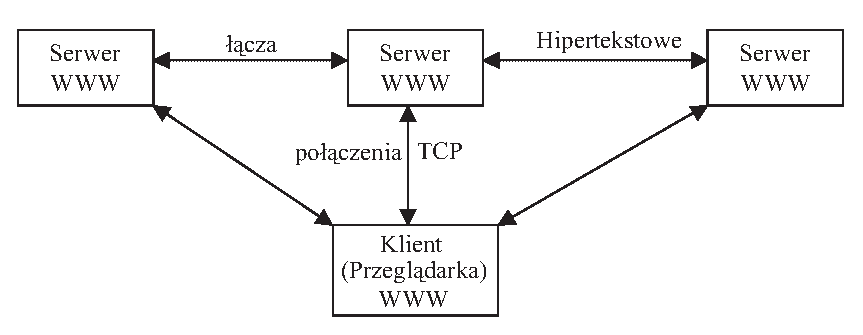
\includegraphics[width=5in]{./rysunki/polaczenia_w_sieci_www.eps}
\caption{Schemat po��cze� w sieci WWW}
\label{polaczenia_www}
\end{figure}

Pierwsza linia odpowiedzi serwera nazywana jest lini� stanu. Rozpoczyna j� okre�lenie wersji HTTP, nast�pnie 
podana jest trzycyfrowa liczba okre�laj�ca kod odpowiedzi, a na ko�cu czytelne dla u�ytkownika wyra�enie. 
Poni�sza tabela przedstawia znaczenie poszczeg�lnych kod�w odpowiedzi.

Starsze specyfikacje protoko�u (HTTP 0.9 i HTTP 1.0) u�ywa�y osobnego po��czenia TCP do pobrania ka�dego 
elementu (pliku) wchodz�cego w sk�ad dokumentu. Najnowsza wersja HTTP 1.1 umo�liwia stosowanie sta�ego, 
podzielonego na sesje po��czenia TCP do pobrania ca�ego dokumentu.

Poni�ej om�wiono istotne ze wzgl�du na wydajno�� WWW cechy protoko�u HTTP.

\subsection{W�a�ciwo�ci ruchu generowanego przez HTTP, a wydajno�� WWW}

W okresie od stycznia 1994 do kwietnia 1995 udzia� komunikat�w HTTP w�r�d wszystkich pakiet�w przesy�anych 
w szkieletowej sieci NSFNET wzr�s� z 3\% do 36\% i warto�� ta wykazywa�a sta�� tendencj� wzrostow�. 

Badania prowadzone w USA wykaza�y niezale�n� od stopnia obci��enia serwera proporcj� pomi�dzy 
poszczeg�lnymi typami ��da� klienta. ��dania typu GET stanowi� ok. 99\% og�u komunikat�w przetwarzanych przez 
serwer. 0,85\% komunikat�w to ��dania typu HEAD. Pozosta�e 0,15\% stanowi� ��dania POST. 

Je�li chodzi o odpowiedzi to 78\% do 92\% stanowi� odpowiedzi typu 20x (odpowiedzi typu ,,sukces''). Odpowied� typu 
304 obejmuj� 4\% do 14\% wysy�anych przez serwer komunikat�w. ��cznie odpowiedzi typu 20x i 304 stanowi� 92\% do 
97\% og�u odpowiedzi. W przypadku pozosta�ych typ�w odpowiedzi r�nice s� ju� znaczne w zale�no�ci od rodzaju 
informacji na serwerze i jego popularno�ci. Np. odpowiedzi 301 i 302 mog� mie� 0,3\% udzia� w odpowiedziach 
popularnego serwera publikuj�cego informacje naukowe NCSA (ang. \emph{National Center for Supercomputer Applications}) 
do nawet 4,2\% w przypadku niewielkiego serwera uniwersyteckiego w Calgary. Odpowiedzi typu 40x i 50x stanowi� 
zwykle od 1\% do 4\%. 

Typowo ilo�� danych przesy�anych w po��czeniu HTTP jest niewielka. ��dania klienta nie przekraczaj� kilkuset 
bajt�w, a pojedyncza odpowied� serwera rzadko kiedy przekracza 10 kB.

Ciekawych informacji dostarczy� mo�e analiza pomiaru czasu RTT (ang. \emph{Round Trip Time}), czyli ��cznego czasu 
wymiany pakietu na drodze serwer -- klient -- serwer. Warto�� ta jest u�ywana przez TCP do wyznaczenia czasu 
retransmisji segmentu w przypadku braku potwierdzenia odbioru. Przybli�enie tego czasu mo�na uzyska� dokonuj�c 
pomiaru czasu trwania fazy zamykania po��czenia TCP. Przytoczone tu wyniki otrzymano mierz�c ten czas dla 19 
ty�. po��cze� wykonanych przez 810 r�nych klient�w na terenie USA. Najmniejsza warto�� wynios�a 0 sekund dla 
hosta lokalnego a najwi�ksza 12,3 sekundy. Warto�� �rednia by�a r�wna 0,445 sekundy a mediana 0,187 sekundy. 
Wyniki te s� zadziwiaj�ce je�li wzi�� pod uwag�, �e teoretyczny RTT pomi�dzy wschodnim i zachodnim wybrze�em USA 
wynosi 0,06 sekundy. Odpowiedzialno�� za ten fakt ponosi� mo�e znaczna ilo�� klient�w pod��czonych poprzez modem 
(najszybszy nawet modem wprowadza ok. 0.2 sekundy op�nienia do ka�dego pojedynczego pomiaru warto�ci RTT). 

Cech� bardzo niekorzystnie wp�ywaj�c� na wydajno�� HTTP w jego starszych wersjach by�a konieczno�� otwierania 
osobnego po��czenia TCP dla ka�dego elementu dokumentu. Wiele zale�a�o tutaj od konstrukcji przegl�darki. Je�li 
nie otwiera�a ona po��cze� r�wnoczesnych to pobranie ca�ego dokumentu wyd�u�a�o si� o czas konieczny na kolejne 
nawi�zywanie i zamykanie po��cze�. Je�li z drugiej strony przegl�darka ,,agresywnie'' otwiera�a zbyt wiele 
po��cze� r�wnoczesnych, to barier� stawa�a si� przepustowo�� po��czenia z Internetem i wielko�� MSS oferowana 
przez serwer. Znany jest przyk�ad przegl�darki NCSA Mosaic, kt�ra potrafi�a otworzy� kilkana�cie r�wnoczesnych 
po��cze� TCP dla pobrania pojedynczego dokumentu, powoduj�c tym zar�wno zatory w sieci lokalnej jak i 
niepotrzebne obci��enie serwera. 

Otwieranie zbyt wielu po��cze� r�wnoczesnych nie przynosi spodziewanych korzy�ci. Podstawowym 
problemem wydajno�ci HTTP wydaje si� by� niedopasowanie protoko�u TCP -- zorientowanego na przesy�anie strumienia 
bajt�w i us�ugi WWW zorientowanej na przesy�anie wyodr�bnionych komunikat�w. Nale�y pami�ta� �e HTTP, kt�ry jest 
w rzeczywisto�ci protoko�em przesy�ania plik�w, mia� w swych za�o�eniach zapewnia� wydajno�� wi�ksz� ni� 
protok� FTP. Chciano uzyska� to eliminuj�c wyst�puj�ce w FTP dodatkowe po��czenie steruj�ce (port 21) i 
konieczno�� nawi�zywania po��czenia TCP na dw�ch portach. 

Niestety TCP wymaga zestawienia po��czenia przed faktycznym rozpocz�ciem transmisji. Wprowadza to op�nienie o 
warto�ci ok. 1 RTT przed przes�aniem pliku. Dodatkowo w starszych wersjach HTTP pobranie dokumentu wymaga�o 
otwieranie nowego po��czenia TCP dla ka�dego pliku sk�adowego, co oznacza, �e nale�a�o zamyka� po��czenia przez 
kt�re wys�ano wcze�niejsze elementy dokumentu. Ka�dorazowe zamykanie i otwieranie po��cze� wprowadza op�nienie 
rz�du 3RTT dla ka�dego pliku sk�adowego. HTTP 1.1 u�ywa sta�ego ��cza TCP dla dokumentu, co zredukowa�o 
op�nienie przed rozpocz�ciem transferu kolejnego elementu dokumentu do 1RTT. Dodatkowo HTTP 1.1 umo�liwia 
wysy�anie ��da� potokowych tzn. wysy�anie ��da� o kolejne pliki przed rozpocz�ciem odbierania poprzednio 
��danych element�w dokumentu. Niestety w przypadku plik�w dynamicznych np. plik�w wynikowych skryptu CGI potok 
taki jest wstrzymywany. 
\chapter{Rozproszone serwery WWW}
\label{r03}
Rozdzia� ten przybli�y architektur� najcz�ciej wykorzystywan� w komunikacji tak pomi�dzy programami jak i
urz�dzeniami sieciowymi: architektur� klient--serwer. Nast�pnie zostanie przedstawiona budowa i dzia�anie serwera
WWW oraz wsp�pracuj�cego z nim klienta -- przegl�darki. Kolejnym punktem tego rozdzia�u b�dzie klasyfikacja
serwer�w WWW ze wzgl�du na wielko�� obs�ugiwanego ruchu jak i na charakterystyk� budowy i wymagania oraz
zwi�zane z tym definicje. W ostatnim punkcie tego rozdzia�u b�dzie przedstawiony spos�b testowania serwer�w webowych.

\section{Wprowadzenie}
Cz�sto�� i wydajno�� dostarczania us�ug WWW, przy stale zwi�kszaj�cej si� ich popularno�ci, 
stanowi nie lada problem dla tradycyjnych rozwi�za� klient--serwer. Zwi�kszenie dost�pno�ci
serwis�w mo�na osiagn�� modyfikuj�c poszczeg�lne elementy na drodze od klienta do serwera 
i/lub dodaj�c nowe. Na rys. \ref{www} przedstawiono cz�� element�w, kt�re wp�ywaj� na wydajno�� 
sieci Web.
\begin{figure}[h]
\centering
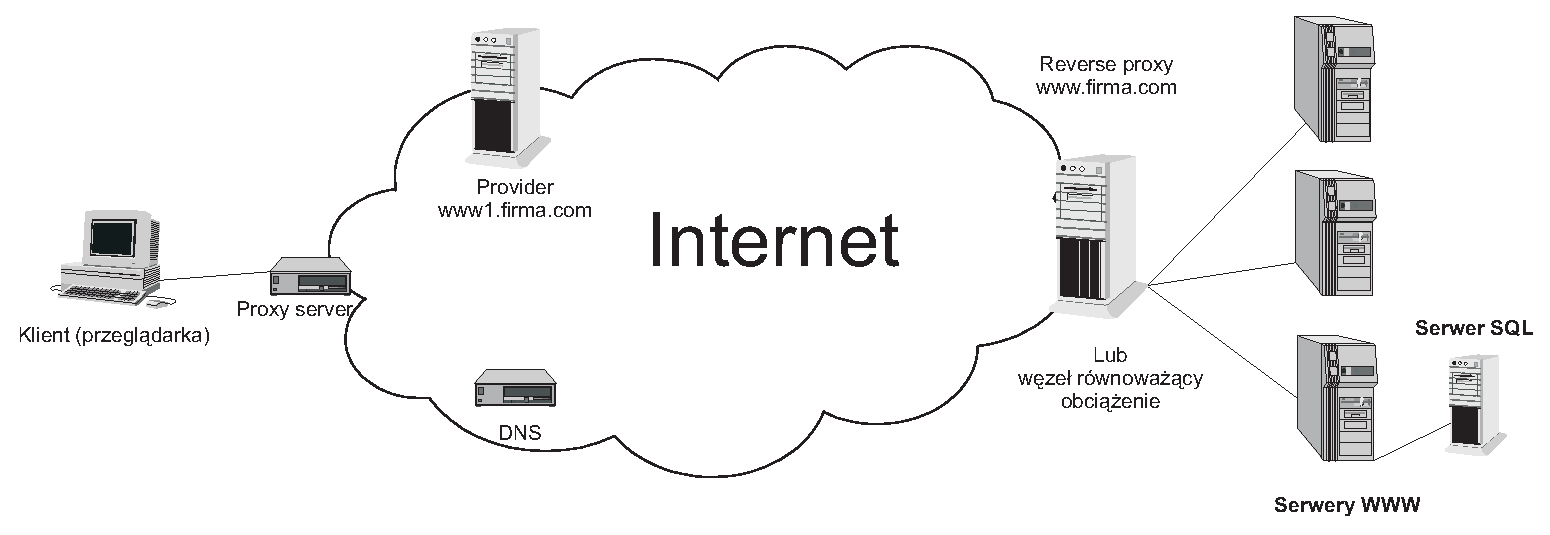
\includegraphics[width=\textwidth]{./rysunki/www.eps}
\caption{Przyk�adowe elementy stanowi�ce o wydajno�ci WWW}
\label{www}
\end{figure}

Najprostszymi s� \emph{cache} przegl�darki lub proxy serwer zainstalowany
po stronie klienta. Takie rozwi�zanie ma wiele zalet: prostota instalacji i konfiguracji, a przy
odpowiednich dokumentach (statyczny HTML) efektywno�� takiego rozwi�zania jest bardzo du�a. 
Wad� tych rozwi�za� jest g��wnie s�aba wydajno�� przy dokumentach generowanych dynamicznie
(a takich obecnie zdarza si� coraz wi�cej). Podobne rozwi�zanie mo�na zastosowa� po stronie 
serwera WWW, tzn. proxy, kt�re keszuje strony po stronie serwera(�w) -- nazywa si� ono 
\emph{reverse proxy}. 

Mo�na tak�e skorzysta� z us�ug r�nych dostawc�w (\emph{provider�w})
i przenie�� cz�� witryny WWW na ich komputery. Efektem b�dzie zwi�kszenie dost�pno�ci 
(oraz wydajno�ci) witryny, jednak�e za cen� mniejszego bezpiecze�stwa i zmniejszenia 
funkcjonalno�ci sajtu.

Mo�na zwi�ksza� wydajno�� w najprostszy spos�b --
poprzez dodawanie kolejnych procesor�w, pami�ci, dysk�w czy te� urz�dze� sieciowych. Jest to 
mo�liwe tylko w bardzo ograniczonym zakresie. 

Wydaje si�, �e najciekawszym rozwi�zaniem
jest wielokomputerowy serwer WWW. Zalet� wykorzystania wielokomputerowego serwera WWW
jest praktycznie nieograniczona skalowalno�� i wysoka dostepno��, wad� natomiast -- 
propagowanie ruchu na poszeg�lne jego sk�adowe (nody). Zarz�dzanie ruchem mo�na realizowa� na
szereg sposob�w: poprzez \emph{reverse proxy}, na poziomie serwera DNS, poprzez osobny w�ze�
r�wnowa��cy obci��enie, modyfikuj�c us�ugi po stronie klienta (opisane dalej applety Java), lub
serwera (metody te zosta�y opisane w rozdziale \ref{r03}). Wraz z architektur� takiego systemu zarz�dzaj�cego serwerem WWW
nale�y zaprojektowa� algorytmy umo�liwiaj�ce rozpraszanie ruchu sieciowego (Rozdzia� \ref{r04}).
Cz�� wy�ej wymienionych rozwi�za� mo�e by� tak iprogramowa jak i sprz�towa.

\section{Model klient--serwer}

\hspace{0.63cm}Model wsp�pracy klient--serwer to taki model, w kt�rym jeden program czeka pasywnie na ��danie komunikacji
wysy�ane przez inne programy. Okre�lenia klient i serwer odpowiadaj� dw�m programom zaanga�owanym w wymian� informacji.
Program inicjuj�cy po��czenie nazywany jest klientem, a program biernie czekaj�cy na ��danie po��czenia -- serwerem. Charakterystyka modelu \cite{siecikomputerowe}:

\begin{description}
\item[Oprogramowanie klienta]\
\begin{itemize}
\item dowolny program u�ytkowy, kt�ry staje si� klientem tymczasowo (w trakcie komunikacji), ale wykonuje r�wnie� obliczenia
lokalnie;
\item jest wywo�ywane bezpo�rednio przez u�ytkownika na czas obejmuj�cy jedn� sesj�;
\item dzia�a lokalnie na urz�dzeniu osobistym u�ytkownika;
\item aktywnie inicjuje po��czenie z serwerem;
\item w razie potrzeby mo�e komunikowa� si� z wieloma serwerami, jednak naraz aktywnie komunikuje si� tylko z jednym;
\item nie wymaga specjalnego sprz�tu, ani spesjalizowanego systemu operacyjnego.
\end{itemize}
\item[Oprogramowanie serwera]\
\begin{itemize}
\item jest specjalizowanym programem, kt�rego zadaniem jest �wiadczenie konkretnej us�ugi -- mo�e obs�ugiwa� naraz wielu
klient�w;
\item jest programem uruchamianym podczas startu systemu i dzia�a przez wiele kolejnych sesji;
\item dzia�a na publicznie dost�pnym komputerze;
\item czeka na zg�aszanie si� program�w klienckich;
\item pe�ni konkretn� us�ug�, ale po��czenia przyjmuje od dowolnych odleg�ych klient�w;
\item wymaga specjalnego sprz�tu i wyrafinowanego systemu operacyjnego.
\end{itemize}
\end{description}

\section{Architektura WWW}

\subsection{Serwer WWW}

\hspace{0.63cm}Najpro�ciej opisa� serwer WWW jako program wykonuj�cy w p�tli prost� operacj�: czekanie na otwarcie po��czenia przez klienta
(przegl�dark�) czyli na wysy�anie przez niego ��dania dost�pu do okre�lonej strony. W odpowiedzi serwer wysy�a ��dany dokument 
(lub komunikat o b��dzie w razie jego braku) albo przekazuje po��czenie do realizacji modu�owi (np. odpowiedzialnemu za obs�ug�
CGI) lub innemu serwerowi (np.: baz danych). nast�pnie serwer zamyka po��czenie i czeka na nast�pne. 

\subsection{Klient WWW -- przegl�darka}

\hspace{0.63cm}Przegl�darki WWW maj� bardziej z�o�on� budow� ni� serwery WWW. Obs�uguje ona wi�kszo�� zagadnie� zwi�zanych
z dost�pem do dokument�w i ich pokazywaniem u�ytkownikowi. W zwi�zku z tym sk�ada si� ona z szeregu du�ych modu��w, kt�re
ze sob� wsp�dzia�aj� \cite{siecikomputerowe}.

Koncepcyjnie przegl�darka sk�ada si� z zestawu klient�w, interpreter�w i modu�u, kt�ry tym wszystkim zarz�dza. Modu�
centralny -- zarz�dzaj�cy jest odpowiedzialny za interpretacj� danych z klawiatury i myszki oraz za wywo�ania pozosta�ych
modu��w w celu wykonania operacji ��danych przez u�ytkownika.

\begin{figure}[h]
\centering
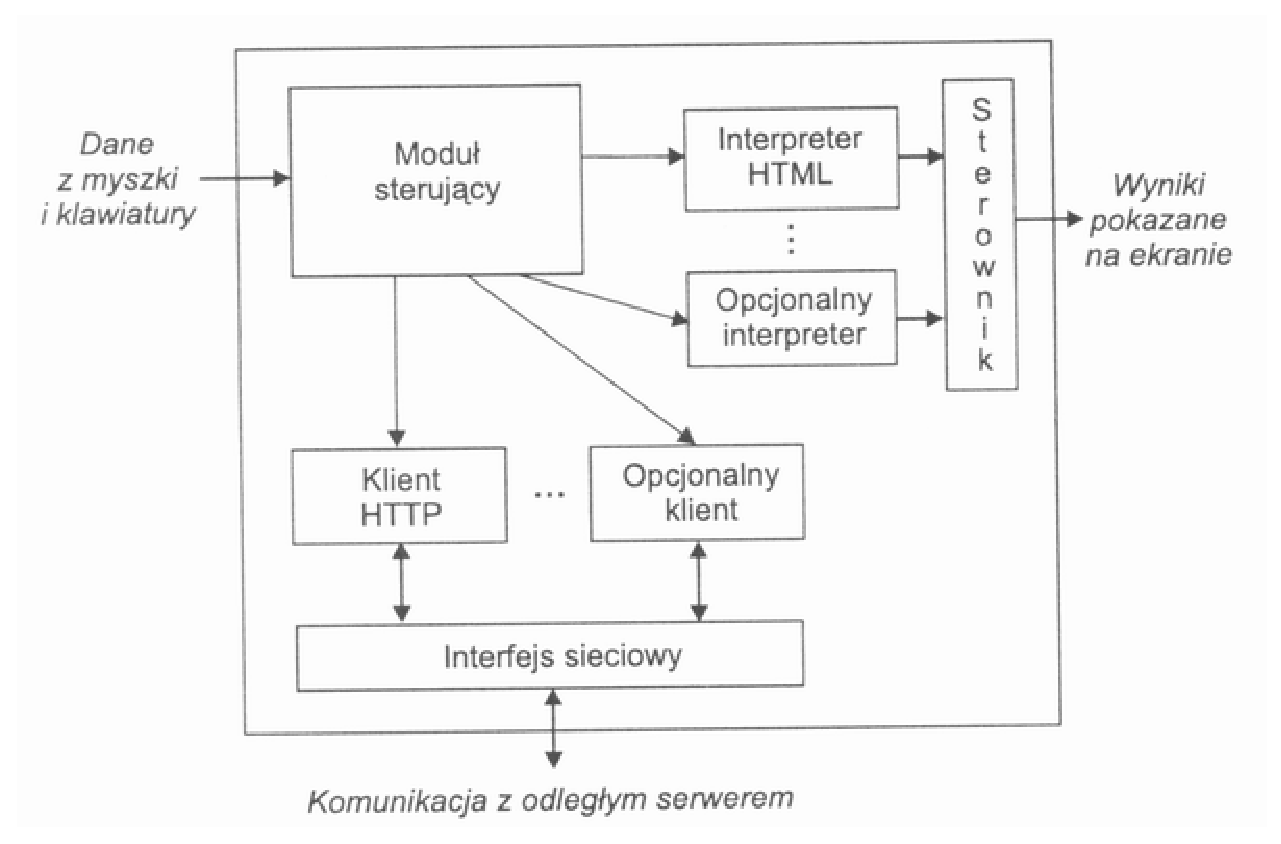
\includegraphics[width=4in]{./rysunki/przeg.eps}
\caption{G��wne sk�adniki przegl�darki WWW}
\label{przegl�darka}
\end{figure}

Ka�da przegl�darka musi zawiera� interpreter j�zyka HTML, �eby w og�le mog�a interpretowa� dokumenty WWW. Inne interpretery
s� opcjonalne, jednak�e powoli staj� si� r�wnie� niezb�dne -- takie jak interpreter Javy, czy XML. Dane dla interpretera
HTML stanowi dokument o zawarto�ci zgodnej ze sk�adni� tego j�zyka; wynikiem jego dzia�ania jest sformatowana posta�
dokumentu przez zamian� znacznik�w formatuj�cych na polecenia steruj�ce sprz�tem wy�wietlaj�cym informacje.

Jedn� z najwa�niejszych funkcji interpretera HTML jest obs�uga fragment�w dokumentu wybieralnych przez u�ytkownika.
Interpreter musi przechowywa� informacje o zwi�zku mi�dzy pozycjami na ekranie, a odsy�aczami w dokumencie HTML. Gdy
u�ytkownik wskazuje za pomoc� myszki pozycj� w dokumencie, interpreter HTML na podstawie bie��cej pozycji kursora i
zapami�tanych informacji ustala, kt�ry odsy�acz wskaza� u�ytkownik.

\subsection{Podzia� serwer�w WWW}

\hspace{0.63cm}Serwery WWW mo�na scharakteryzowa� g��wnie poprzez wielko�� (ilo�� realizacji ��da�) \cite{wybraneelementy}:
\begin{description}
\item[ma�e] -- uruchamiane na stacjach roboczych, zdolne do obs�u�enia do 5000 zapyta� dziennie, np.: prezentuj�ce dane jakiej�
niewielkiej firmy;
\item[�rednie] -- uruchamiane na du�ych serwerach posiadaj�cych zabezpieczenia na poziomie urz�dze� wewn�trznych. Obs�uguj�
kilkadziesi�t tysi�cy ��da� dziennie. Prezentuj� dane (tysi�ce stron) �redniej firmy;
\item[du�e] -- uruchamiane na serwerach o du�ej mocy obliczeniowej (zwykle kilku) posiadaj�cych techniki zabezpieczenia
danych i pracy serwer�w. S� w stanie obs�u�y� kilkaset tysi�cy zapyta� dziennie (prezentuj� kilkaset tysi�cy stron);
\item[globalne] -- s� w stanie obs�u�y� milion ��da� klienckich dziennie, prawie zawsze zbudowane z wielu du�ych serwer�w, 
posiadaj�ce kilka kopii dokumentu. S� wstanie udost�pnia� ogromne ilo�ci danych , r�wnie� multimedialnych.
\end{description}
W zale�no�ci od zawarto�ci witryn definiuje si� trzy klasy obci��alno�ci serwer�w WWW \cite{ScalableWebClusters}. Mamy zatem 
witryny typu:
\begin{description}
\item[web publishing] -- witryny zawieraj�ce statyczne i w niewiekiej ilo�ci dynamiczne dokumenty. Dokumenty statyczne s� 
sk�adowane na dyskach serwera webowego i nie podlegaj� modyfikacjom przez relatywnie d�ugi czas i zawsze s� przechowywane w 
pami�ci podr�cznej. Pami�� podr�czna ka�dego nodu klastra jest zwykle ustawiona na 15\% ca�kowitego drzewa dokument�w witryny.
Strony w niewielkim stopniu dynamiczne s� przechowywane w pami�ci podr�cznej (cache) z pradopodobie�stwem 0,3.
\item[web transaction (light)] -- s� to witryny zawieraj�ce oko�o 60\% dokument�w statycznych i oko�o 40\% stworzonych 
dynamicznie dokument�w. Zapytania bazodanowe do serwer�w \emph{back--endowych} wymagaj� intensywanego korzystania z dysk�w i 
st�d rezultaty zapyta� nie s� przechowywane w keszu.
\item[web transaction (heavy)] -- witryny zawieraj�ce 30\% statycznych dokument�w, 30\% niewiele zdynamizowanych dokument�w
oraz r�ne kombinacje (dla pozosta�ych 40\%) dokument�w, zwykle zawieraj�cych elementy wymagaj�ce sporych mocy obliczeniowych 
CPU i/lub dysku.
\end{description}

\section{Charakterystyka wydajno�ci serwera WWW}

Podstawow� miar� obci��enia serwera WWW jest ilo�� ��da� HTTP, kt�re docieraj� do niego w ci�gu sekundy. 
Za miar� wydajno�ci serwera mo�na przyj�� widziany od strony klienta czas odpowiedzi na ��danie lub czas 
uko�czenia transferu dokumentu, kt�ry zale�ny jest jednak od przepustowo�ci po��czenia klienta z Internetem. 
Przeprowadzone w USA symulacje z u�yciem prostego modelu serwera WWW, kt�ry oparto o teori� kolejek i za�o�enie, 
�e istotne s� tylko ��dania typu GET, s� podstaw� do przedstawienia poni�szych charakterystyk.
Typowo czas odpowiedzi na ��danie ro�nie wraz ze wzrostem liczby ��da� na sekund�. Wzrost ten jest 
pocz�tkowo bardzo powolny, niemal niezauwa�alny a� do momentu, w kt�rym ilo�� r�wnocze�nie otwartych po��cze� 
TCP przekracza mo�liwo�ci obs�ugi ich przez serwer. Przedstawia rysunek \ref{zapytania}[26].
\begin{figure}[h]
\centering
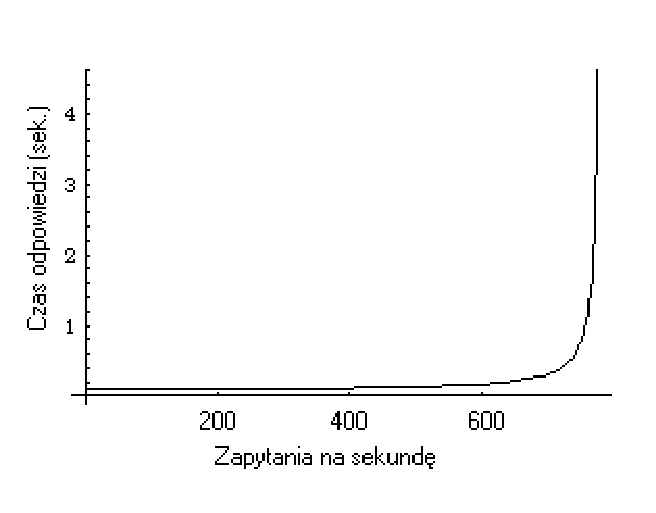
\includegraphics[width=3in]{./rysunki/zapytania.eps}
\caption{Czas odpowiedzi a ilo�� zapyta� na sekund�.}
\label{zapytania}
\end{figure}

Obci��enie przy kt�rym serwer za�amuje si� zale�y oczywi�cie od 
sprz�towych w�asno�ci serwera i zastosowanego oprogramowania. Opr�cz cech samego serwera najistotniejsze dla 
czasu odpowiedzi s� przepustowo�� po��czenia z Internetem oraz �redni rozmiar plik�w wysy�anych przez serwer. 
�redni rozmiar pliku zale�y w g��wnej mierze od rodzaju informacji publikowanych na serwerze (b�dzie on np. du�y 
na serwerze oferuj�cym wiele plik�w video). Po��dane jest jednak ,,oszcz�dne'' projektowanie stron WWW, gdy� 
wzrost �redniego rozmiaru pliku powoduje szybki spadek ilo�ci zapyta� na sekund� mo�liwych do obs�u�enia. 
Opisane zachowanie 
serwera powoduj�ce za�amanie si� jego wydajno�ci po przekroczeniu maksymalnej liczby zapyta� na sekund� jest 
typowe dla implementacji nie posiadaj�cych ograniczenia na maksymaln� liczb� jednoczesnych po��cze� TCP. Dotyczy 
to wi�kszo�ci system�w UNIX--owych, w kt�rych procesy serwer�w WWW wykonuj� standardow� akcj� fork--and--exec dla 
ka�dego nowego ��dania HTTP. Prostym rozwi�zaniem tego problemu wydaje si� wprowadzenie ograniczenia na liczb� 
po��cze� TCP. Wymaga�oby to jednak zmian w protokole HTTP (np. wprowadzenie odpowiedzi typu ,,serwer zaj�ty --
spr�buj p�niej'') oraz odpowiednich zmian w przegl�darkach.

Powy�sze rozwa�ania dotycz� wydajno�ci serwera widzianej od strony klienta. W przypadku laboratoryjnych 
bada� wydajno�ci �atwiej ni� czas odpowiedzi mo�na zmierzy� ilo�� zapyta� na sekund� obs�ugiwan� przez serwer. 
Jest to miara wydajno�ci bezpo�rednio koresponduj�ca z czasem odpowiedzi serwera (im wi�cej zapyta� serwer mo�e 
obs�u�y�, tym mniejszy jest jego czas reakcji) i wolna od wp�ywu takich czynnik�w jak wydajno�� przy��cza po 
stronie klienta.
Ci�g�y wzrost liczby u�ytkownik�w Internetu stawia coraz wi�ksze wymagania co do wydajno�ci serwer�w WWW. Do tego faktu dochodzi jeszcze jeden - charakterystyka ruchu WWW - opr�cz serwowania stron statycznych, dochodz� dynamiczne i obs�uga po��cze� szyfrowanych. 
W jaki spos�b zmienia si� wtedy wykorzystanie poszczeg�lnych element�w wida� na rys.\ref{charakterystyka}
\begin{figure}[h]
\centering
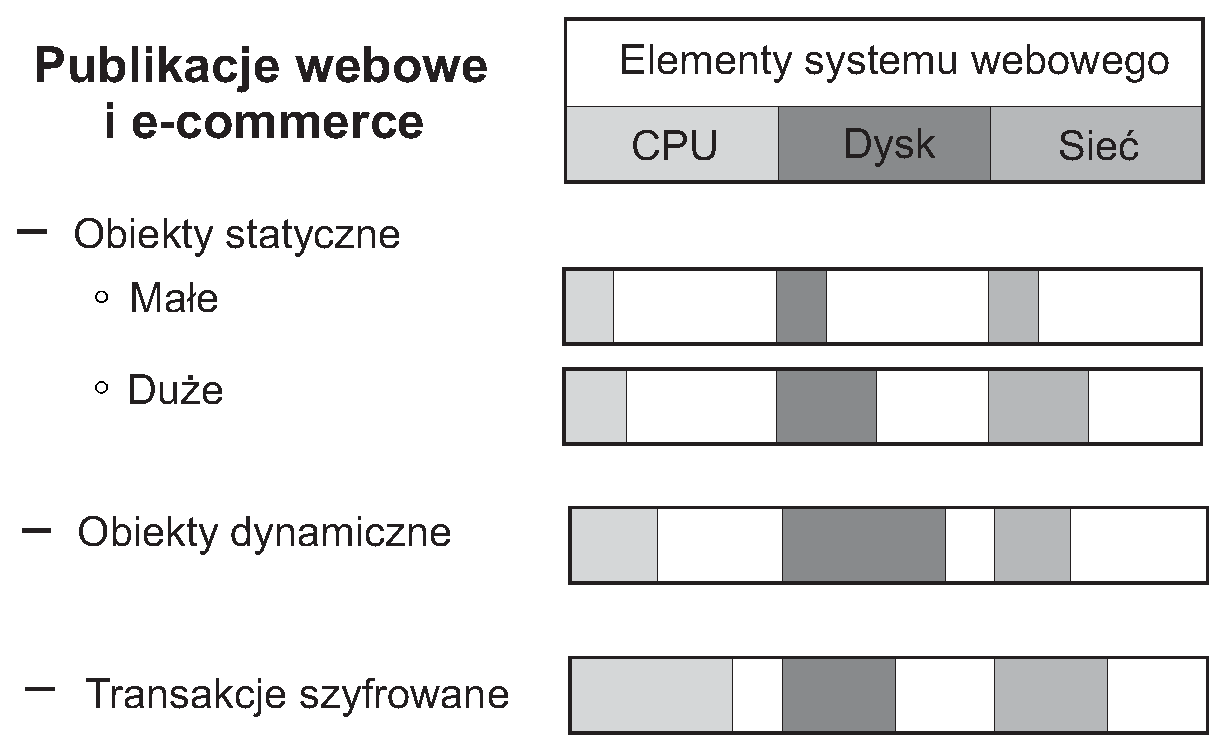
\includegraphics[width=3in]{./rysunki/charakterystyka_ruchu.eps}
\caption{Obci��enie poszczeg�lnych element�w serwera WWW w zale�no�ci od typu po��czenia.}
\label{charakterystyka}
\end{figure}

Pr�dzej czy p�niej ka�dy administrator takiego serwera stanie przed problemem znalezienia sposobu na 
zwi�kszenie jego wydajno�ci. Zwykle ze wzgl�du na specyfik� publikowanych informacji niewiele mo�na zrobi� ze 
�rednim rozmiarem przesy�anego pliku. Podstawow� metod� zwi�kszenia wydajno�ci serwera jest zwi�kszenie 
przepustowo�ci przy��cza. Sprz�towa modernizacja samego serwera nie przyniesie rezultat�w w przypadku gdy 
,,w�skim gard�emi'' jest przy��cze. Je�li jednak dysponujemy odpowiednio wydajnym przy��czem (np. lini� ATM) 
,,w�skim gard�em'' jest na pewno serwer. 

Wydajno�� ka�dego komputera zwi�kszy� mo�na dokupuj�c wi�ksz� ilo�� pami�ci RAM i szybsze dyski twarde. 
W przypadku serwer�w WWW jest to jednak rozwi�zanie prowizoryczne. Lepsze efekty przynosi instalacja maszyny 
wieloprocesorowej. Niestety obecne implementacje TCP/IP nie wykorzystuj� wielow�tkowo�ci w stopniu, kt�ry 
umo�liwia�by pe�ne wykorzystanie cech technologii wieloprocesorowej. Nale�y si� spodziewa�, �e otwartych 
po��cze� TCP b�dzie typowo wi�cej ni� procesor�w w serwerze. Gdyby obs�ug� stosu TCP/IP podzieli� mo�na by�o na 
niezale�ne w�tki, kt�rych wykonanie przebiega� by mog�o z podzia�em czasu, to efektywno�� wieloprocesorowych 
serwer�w WWW by�aby znacznie wi�ksza ni� obecnie. Wsp�cze�nie stosowanie serwer�w wieloprocesorowych nie 
przynosi korzy�ci tak du�ych jak spodziewane. 
Dobr� metod� zwi�kszenia wydajno�ci WWW jest stosowanie serwer�w proxy, kt�re na zasadzie pami�ci cache 
przechowuj� cz�� dokument�w serwisu i w ten spos�b cz�ciowo wyr�czaj� serwer g��wny. 
Najbardziej efektywn� i jednocze�nie najbardziej zaawansowan� technologicznie metod� zwi�kszenia 
wydajno�ci serwera WWW jest powielenie jego zawarto�ci na jeden lub kilka dodatkowych serwer�w i udost�pnienie 
tej grupy pod jednym adresem IP. Rozwi�zanie takie wymaga sprz�tu lub oprogramowania, kt�re z jednej strony 
ukrywa�oby przed u�ytkownikami istnienie kilku serwer�w o jednakowej zawarto�ci a z drugiej dokonywa�oby 
dystrybucji obci��enia pomi�dzy te serwery w spos�b maksymalizuj�cy ich ��czn� wydajno��.

\subsection{Serwery wielokomputerowe -- rozproszone}

\hspace{0.63cm}�eby serwery WWW by�y wydajne oraz mog�y pracowa� bez przerwy przez 365 dni w roku 24 godz. 
na dob� -- nie mog� pracowa� na jednym komputerze; wydajno��, skalowalno�� a przede wszystkim odporno�� na 
awarie mo�e zosta� zrealizowana jedynie poprzez rozproszone serwery WWW, w kt�rych zapytania od klient�w s�
w odpowiedni spos�b dystrybuowane do poszczeg�lnych serwer�w \cite{metodyalgorytmy}. 

�wiatowy trend w wykorzystywaniu na r�ne sposoby technologii World Wide Web jest coraz wi�kszy.
Znakomite darmowe serwery WWW (Apache, NCSA itp.), spora ilo�� przegl�darek internetowych
oraz olbrzymi rozw�j internetu \cite{siecikomputerowe}, a tak�e ogrone mo�liwo�ci tej us�ugi spowodowa�y zwi�kszone 
zainteresowanie t� technologi�.
Jednym z ostatnich nies�ychanie modnych technologii internetowych wykorzystuj�cych WWW jest handel 
elektroniczny skierowany tak do pojedynczego odbiorcy (\emph{Business to Customer-- B2C}) jak i wsp�pracuj�cych
firm (\emph{Business to Business}-- B2B). Poza tym r�wnie� bardzo interesuj�cym celem s� serwery aplikacyjne.
Powoduje to jednak�e konieczno�� utrzymania w sprawno�ci serwisu przez ca�y rok -- bez 
przerwy. Nie oznacza to wy��cznie mo�liwo�ci korzystania z tych serwer�w, czyli bezawaryjnej pracy, ale r�wnie�
uzyskanie jak najlepszego komfortu pracy z tymi systemami. Poza tym jeszcze jedn� nies�ychanie istotn� rzecz�
przemawiaj�c� za wielokomputerowymi serwerami WWW jest ich znakomita skalowalno�� (du�o ta�sza od skalowalno�ci
pojedynczych maszyn, kt�re nie zawsze dadz� si� rozbudowywa�). Takich zalet nie posiada pojedyncza maszyna. Jej koszt zakupu, 
a tak�e koszt rozbudowy -- przy zapewnieniu bezpiecze�stwa i odporno�ci na uszkodzenia jest olbrzymi. Fakt, �e pojedyncz�
maszyn� �atwiej si� administruje nie rekompensuje w pe�ni u�omno�ci architektury von Neumanna. Wielokomputerowe serwery
(nie tylko WWW, ale tak�e serwery obliczeniowe) mog� osi�ga� zawrotne wydajno�ci, s� praktycznie w niesko�czono�� skalowalne,
nadmiarowo�� tanich element�w (zamiast kupowa� trzy maszyny klasy mainframe -- mo�na kupi� sto komputer�w klasy PC) decyduje
o ich odporno�ci na uszkodzenia. Najlepszym przyk�adem jako�ci tej technologii jest najpot�niejsza z wyszukiwarek sieciowych --
GOOGLE\footnote{\emph{www.google.com}} pracuj�ca na kilku tysi�cach komputerow klasy PC, a zawieraj�ca w swojej bazie informacje 
o ponad miliardzie trzystu milionach stron WWW (jest wykorzystywana przez wi�kszo�� serwis�w webowych). Wad�
system�w klastrowych jest administracja i spos�b wsp�dzielenia obci��enia pomi�dzy poszczeg�lnymi nodami (istnieje jednak�e
oprogramowanie darmowe umo�liwiaj�ce r�wnowa�enie obci��enia serwer�w WWW\footnote{\emph{www.linuxvirtualserver.org}}, a 
tak�e serwer�w obliczeniowych\footnote{\emph{www.mosix.org}}).

Trend ten nie znajduje odzwierciedlenia tylko w serwerach webowych. Konstrukcja wielokomputerowa pozwala na znacznie 
efektywniejsze zarz�dzanie zasobami i przydzieleniem zada� do zasob�w. Pozwala tak�e uzyska� ,,prawdziwe'' zr�wnoleglenie
oblicze� -- brak jest tu ,,kombinowanych'' metod uwsp�lniania zasob�w i rozdzia�u ��da� do magistral i pami�ci obecnych
w typowych architekturach. Kolejn� zalet� system�w nieneumanowskich jest mo�liwo�� zapewnienia bezpiecze�stwa ci�g�o�ci
pracy w spos�b dot�d niewykonalny. Przyk�adem spe�nienia wszystkich tych cech s� wsp�czesne superkomputery i mainframy, 
z kt�rych do�wiadcze� korzystali wsp�cze�ni tw�rcy nowoczesnych, skalowalnych technik webowych. Ka�dy superkomputer (SGI,
Hitachi, NEC, Intel, IBM) oraz system mainframowy (g��wnie IBM) sk�ada si� z szeregu (nawet kilkudziesi�ciu) nod�w 
skonsolidowanych zwykle w jednej obudowie, a po��czonych wysokoprzepustow� sieci� transmisyjn�. St�d wiele pomys��w zosta�o
zaczerpni�tych i wykorzystanych przy tworzeniu rozposzonych architektur webowych.

Klasyczny system komputerowy obs�uguj�cy serwer webowy jest obs�ugiwany niskopoziomowo -- system operacyjny obs�uguj�cy
serwer webowy. W architekturze rozproszonego webu pomi�dzy systemem operacyjnym poszczeg�lnych nod�w, a serwerem WWW (r�wnie�
poszczeg�lnych nod�w) znajduje si� logiczny uk�ad koordynuj�cy dzia�ania poszczeg�lnych serwer�w WWW tak aby dzia�a�y jako
jeden rozproszony serwis. Ten system zarz�dzaj�cy odpowiada za: 
\begin{itemize}
\item rozdysponowywanie ��da� przychodz�cych od klient�w na poszczeg�lne nody w taki spos�b aby zapewni� zr�wnowa�enie 
obci��enia poszczeg�lnych maszyn, 
\item zapewnienie sp�jno�ci danych na drodze klient--serwer www--klient, 
\item oraz sprawowanie kontroli nad poszczeg�lnymi elementami klastra w ten spos�b, aby zawsze, i odpowiednio szybko, by�o 
wiadomo, kt�ry komputer nale�y omija� ze wzgl�du na awari�.
\end{itemize}

Poni�ej znajduje si� opis i charakterystyka poszczeg�lnych system�w r�wnowa��cych obci��enia w rozproszonych serwerach 
webowych. 

\section{Przegl�d skalowalnych system�w serwer�w webowych}

Na rysunku \ref{proste_modele} przedstawiono wszystkie proste modele funkcjonalne system�w do r�wnowa�enia obci��e� w serwisach WWW. 
Ich charakterystyczn� cech� jest to, i� w ka�dym wykorzystywany jest jeden mechanizm szeregowania. Mo�na je traktowa� jak 
swego rodzaju klocki, z kt�rych budowane s� rzeczywiste systemy. Cze�� z nich odpowiada rzeczywistym systemom bez dodatkowych 
modyfikacji, cz�� odzwierciedla rzeczywiste systemy dopiero we wzajemnych kombinacjach. Wyodr�bnienie prostych modeli 
umo�liwia zbudowanie przejrzystej taksonomii skalowalnych system�w serwer�w webowych.

\begin{figure}[h]
\centering
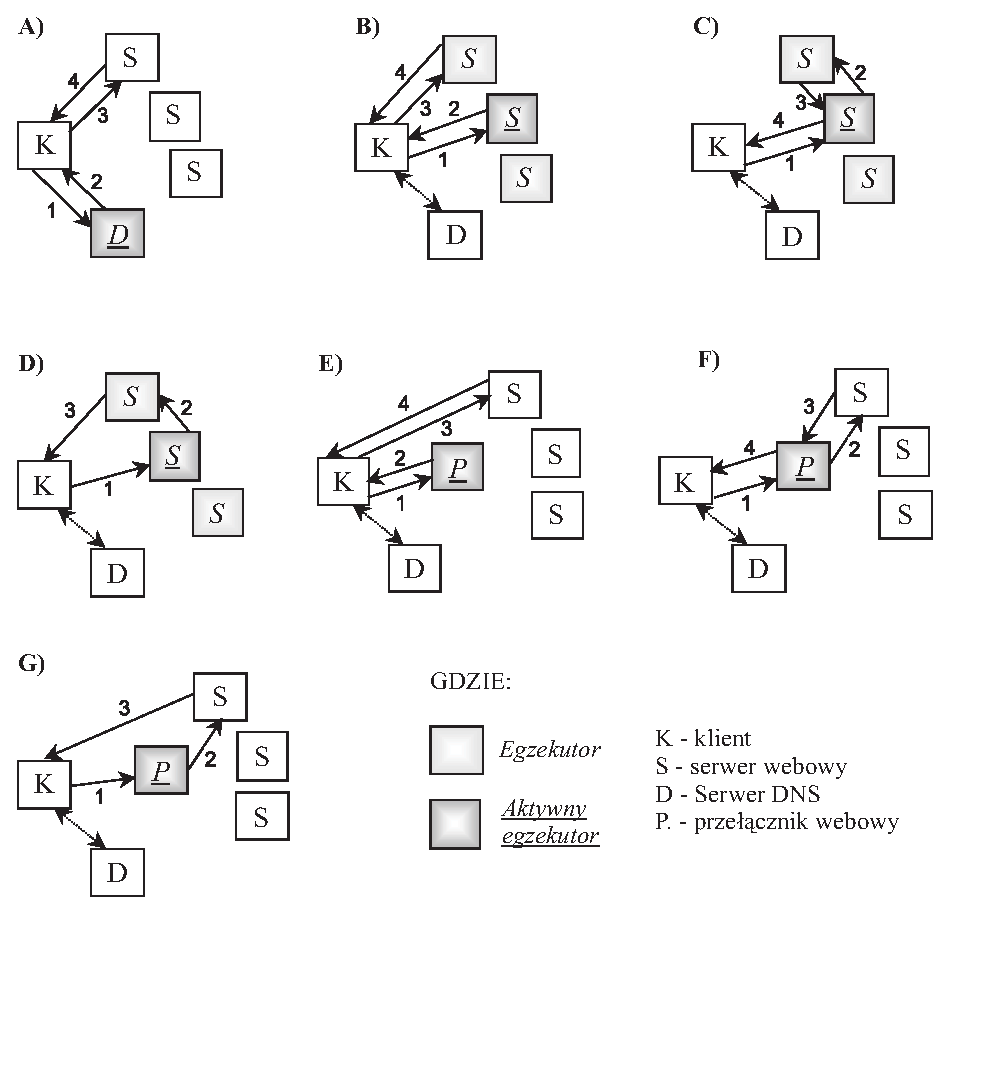
\includegraphics[width=4.9in]{./rysunki/modele_podstawowe.eps}
\caption{Podstawowe modele system�w do r�wnowa�enia obci��e�}
\label{proste_modele}
\end{figure}

\subsection{Podzia� ze wzgl�du na rozmieszczenie serwer�w webowych}
Podzia� ten kszta�tuje si� nast�puj�co:
\begin{itemize}
\item Klaster webowy. Je�li serwery webowe s� rozproszone lokalnie (skupione geograficznie), to m�wi si� o tzw. klastrze 
webowym (web--cluster). Z technicznego punktu widzenia klaster webowy funkcjonuje w obr�bie sieci lokalnej. Ka�dy z prostych 
modeli przedstawionych na rys.\ref{proste_modele} mo�e by� implementowany w klastrze webowym. W przypadku modelu {\bf G}, ze wzgl�du na uwarunkowania 
techniczne transmisji ��da�, mo�e zaj�� potrzeba umiejscowienia klastra w obr�bie podsieci sieci 
lokalnej \cite{modele15,modele20,LoadBalancingWithND}.
\item Rozproszone serwery webowe. Je�li mi�dzy rozproszonymi globalnie (rozproszonymi geograficznie) serwerami webowymi 
stosowany jest jakikolwiek mechanizm szeregowania, m�wi si� o rozproszonych serwerach webowych (distributed web--servers), w 
przeciwnym przypadku -- o lustrzanych serwerach webowych (mirror web--servers). Teoretycznie ka�dy model przedstawiony na rys.\ref{proste_modele}
mo�e by� implementowany w�r�d rozproszonych serwer�w webowych, jednak ze wzgl�du na powstawanie dodatkowych op�nie� podczas 
transmisji zwrotnej w modelu {\bf F} oraz uwarunkowania techniczne transmisji ��da� w modelu {\bf G}, oba wymienione modele maj� 
zastosowanie g��wnie klastrach webowych.
\item Rozproszone klastry webowe. Szczeg�lnym przypadkiem rozmieszczenia serwer�w webowych jest kombinacja globalnego i 
lokalnego rozproszenia. Je�li miedzy klastrami webowymi stosowany jest jakikolwiek mechanizm szeregowania, m�wi si� o 
rozproszonych klastrach webowych (distributed web--clusters). W przeciwnym przypadku -- o lustrzanych klastrach webowych (mirror 
web--clusters). Rozproszone klastry webowe mo�na przedstawia� za pomoc� kombinacji prostych modeli funkcjonalnych (rys.\ref{complex_modele} {\bf J, K}). 
\end{itemize}

\subsection{Podzia� i charakterystyka ze wzgl�du na umiejscowienie mechanizmu szeregowania}

Mechanizm szeregowania mo�e by� umiejscowiony: po stronie klienta, po stronie serwera, oraz jako osobny uk�adu (serwer DNS,
dystrybutor).

\subsubsection{Podej�cie od strony klienta}

G��wn� zalet� stosowania mechanizm�w rozpraszania obci��enia po stronie klienta jest ca�kowita niezale�no�� od architektury 
serwera(�w), a przede wszystkim od miejsca ich rozmieszczenia (mog� by� nie tyle geograficznie rozproszone, co wr�cz 
nieskoordynowane jako ca�o��). 

Rozwi�zania w tym zakresie mo�emy podzieli� na dwie podgrupy:
\begin{itemize}
\item mechanizmy r�wnowa�enia obci��enia implementowane w przegl�darkach i jako applety Java:
\begin{itemize}
\item w przegl�darkach poprzez API. Przegl�darka mo�e aktywnie pe�ni� role� w dystrybucji zapyta�, pod warunkiem posiadania
informacji na temat adres�w serwer�w WWW. Wtedy, na podstawie zapytania otrzymanego od u�ytkownika, przegl�darka wybiera
serwer do przed�o�enia zapytania. Klasycznym przyk�adem takiego rozwi�zania jest mechanizm LB implementowany w przegl�darkach
firmy Netscape \cite{gliwice16,gliwice17}. Po wygenerowaniu zapytania przez u�ytkownika (tylko do serwera 
www.netscape.com), przegl�darka wybiera liczb� z zakresu od 1 do liczby znanych jej serwer�w i kieruje zapytanie do w�z�a
o adresie www\emph{liczba}.netscape.com. Nie jest to rozwi�zanie interesuj�ce, gdy� liczba serwer�w i adres�w jest na sta�e 
zakodowana w przegl�darce. Poza tym taki spos�b rozdysponowywania ruchu (losowy) nie zapewnia r�wnowa�enia obci��enia pomi�dzy
serwerami;
\item applety Java. O wiele ciekawszym od powy�szego rozwi�zaniem, jest implementacja specyficznych applet�w Java. Gdy
u�ytkownik wysy�a ��danie do serwisu, zamiast dokumentu HTML, pobiera applet Java. Applet ten zawiera adresy IP maszyn 
dostarczaj�cych ten serwis WWW \cite{gliwice18,gliwice19}. Applet mo�e by� modyfikowany przez program zbieraj�cy informacje o 
stanie serwer�w (o ich obci��eniu) oraz o jako�ci po��czenia sieciowego. Informacje te mo�e wykorzystywa� applet do
wyboru najbardziej odpowiedniego serwera do realizacji ��dania. G��wn� wad� tego rozwi�zanie jest generowanie 
dodatkowego ruchu w sieci (zwi�zanej z pobieraniem informacji o stanie obci��enia serwer�w. Naturalnie jest ono r�wnie� 
bezu�yteczne gdy przegl�darka nie potrafi interpretowa� kodu Javy.
\end{itemize}
\item serwery Proxy. Jest to oparte na pomy�le po raz pierwszy wykorzystanym przez badaczy z Cambridge 
University \cite{gliwice20}. Mechanizm, kt�ry zosta� zaimplementowany w serwer proxy, bazuje na informacji o 
osi�gni�tej wydajno�ci podczas dotychczasowych transmisji. Klient otrzymuje list� zreplikowanych serwer�w postrzeganych przez
u�ytkownika pod jednym adresem. Ka�dej pozycji na li�cie jest przypisana informacja o wydajno�ci serwera. Za ka�dym razem, 
gdy klient utworzy po��czenie z serwerem jest ona aktualizowana. Wybierany jest mirror na podstawie znajomo�ci
najlepszej ze �rednich wydajno�ci serwera w ci�gu ostatnich transmisji. Decyzja jest podejmowana z zastrze�eniami: je�li 
wydajno�� ostatniej transmisji spad�a poni�ej pewnego progu, serwer jest uwa�any za nieosi�galny. Wyb�r serwera proxy
wynika� z kilku wa�nych powod�w: ukrycie przed u�ytkownikiem faktu wyboru dokumentu mi�dzy zreplikowanymi serwerami, brak
konieczno�ci ingerencji w kod przegl�darki, oraz korzy�� w postaci wsp�dzielenia informacji o wydajno�ci zreplikowanych 
serwer�w mi�dzy u�ytkownikami przegl�darek. Kilku klient�w generuje wi�ksz� liczb� zapyta�, poprawiaj�c w ten spos�b wydajno��
algorytmu r�wnowa�enia obci��enia \cite{gliwice20}. 
\end{itemize}

\subsubsection{Podej�cie od strony serwera}

Techniki r�wnowa��ce obci��enie w oparciu o serwery wykorzystuj� dwupoziomowy mechanizm dystrybucji. Najpierw zapytania
klienta s� przydzielane serwerom webowy w klastrze poprzez DNS. Nast�pnie ka�dy serwer mo�e przekaza� otrzymane zapytanie
do innego serwera w klastrze. Rozwi�zanie w oparciu o rozproszone szeregowanie pozwala wszystkim serwerom bra� udzia�
w r�wnowa�eniu obci��enia w klastrze poprzez mechanizm przekazywania zapyta�. Po��czenie podej�cia w oparciu o DNS oraz z
technikami przekierowywania zapyta� poprzez serwery webowe prowadzi do rozwi�zania wi�kszo�ci problem�w wynikaj�cych z polityki
szeregowania np.: niejednolita dystrybucja zapyta� wewn�trz domeny, czy ograniczona kontrola nad zapytaniami.

Propozycje oparte na przekierowaniach serwer�w r�ni� si� w sposobie podejmowania decyzji. W nast�pnym rozdziale s� 
przedstawione dwie g��wne klasy rozwi�za�: wykorzystuj�ce funkcje redirekcji na poziomie protoko�u HTTP oraz w oparciu o
mechanizm przepisywania pakiet�w. 

\subsubsection{Podej�cie od strony niezale�nego w�z�a dystrybuuj�cego zapytania}

W wyniku zapytania klienta o dane z serwera WWW -- w pierwszej kolejno�ci nast�puje rozwini�cie nazwy domenowej serwera na
jego adres IP. Nast�pnie adres IP mo�e by� reprezentowany przez wirtualny adres IP przypisany do klastra serwer�w. Samo
rozwini�cie IP w adres serwera mo�e by� realizowane na r�nych poziomach. Mo�e to by� przekierowanie do konkretnych zasob�w na 
poziomie protoko�u HTTP \cite{modele2} lub na poziomie protoko�u IP oraz adresu URL przy zastosowaniu 
dystrybutora \cite{modele1,gliwice3}.

Na pocz�tku skupiano si� na rozwi�zaniach dotycz�cych podmiany nazwy serwisu na jego adres IP \cite{gliwice4}. Jednak�e w 
zwi�zku z faktem ogranicze� takiego rozwi�zania coraz wi�ksz� uwag� po�wi�ca si� implementacji mechanizm�w podmiany 
wirtualnego adresu IP na adres konkretnego hosta. Przyk�adami takiego podej�cia s�: Berkeley MagicRouter \cite{modele1}, 
CISCO Local Director \cite{gliwice13}, VirtualServer \cite{virtualserver} oraz IBM SecureWay Network Dispatcher \cite{GettingStarted}.

\begin{itemize}
\item Wykorzystanie serwera DNS -- 
egzekutorem jest serwer DNS lub inne urz�dzenie wspomagaj�ce albo przejmuj�ce rol� serwera DNS. Nale�y u�ci�li�, 
�e chodzi tu o tzw. g��wny serwer DNS b�d�cy autorytatywnym �r�d�em informacji o okre�lonej domenie (\emph{authoritative DNS}).
Jak opisano w Rozdziale 2 system DNS s�u�y do odwzorowania symbolicznych nazw komputer�w w Internecie na ich 
adresy IP. Funkcja ta, w niejako naturalny spos�b, czyni serwer DNS dobrym miejscem na implementacj� mechanizmu 
r�wnowa�enia obci��e�. Pierwsz� instalacj� wykorzystuj�c�  DNS do r�wnowa�enia obci��e� by� serwis WWW NCSA 
(ang. \emph{National Center for Supercomputing Applications}). Zestawiono tam klaster dziewi�ciu serwer�w WWW, kt�ry 
stanowi� odr�bny obszar DNS i by� udost�pniany pod nazw� www.ncsa.ninc.edu \cite{barylo28,barylo29}. Na podstawowym serwerze 
DNS  domeny (obszaru) ncsa.ninc.edu skonfigurowano oprogramowanie, kt�re na zapytania o odwzorowanie nazwy 
www.ncsa.ninc.edu odpowiada�o podaj�c cyklicznie adresy kolejnych serwer�w z klastera. Ten statyczny algorytm 
nazywany jest cyklicznym DNS lub RR--DNS (ang. \emph{Round--Robin DNS}). 

Podej�cie to jednak bardziej realizuje rozproszenie strumienia zapyta� klient�w ni� r�wnowa�enie obci��enia serwer�w WWW. W
rzeczywisto�ci w Internecie jest wiele serwer�w DNA i maj� one uk�ad hierarchiczny tzn. nie zawsze trzeba sprawdza� adres IP
w docelowym serwerze DNS. Oznacza to, �e nie mamy wp�ywu na cz�� zapyta�, jakie s� kierowane do serwera. W pewnym stopniu
poprawia sytuacj� zastosowanie sygna��w zwrotnych od serwera WWW do serwera DNS o przeci��eniu. Efekt jest odczuwalny dopiero 
po up�ywie czasu TTL (np. w momencie uszkodzenia maszyny i wy��czenia jej adresu z puli adres�w serwera DNS). Aby efektywno��
tego typu rozwi�za� by�a jak najwi�ksza, wa�ne jest prawid�owe oszacowanie tzw. ukrytego obci��enia, czyli wielko�ci zapyta�
nap�ywaj�cego w czasie TTL. Do estymowania tej wielko�ci mo�na zastosowa� funkcje heurystyczne \cite{gliwice4}.

\item Reverse proxy serwer

Typowe forward proxy (tak�e transparent) zwykle u�ywane przez prowajder�w internetu przechowuj� strony najcz�ciej pobierane 
przez u�ytkownik�w. Z reverse proxy firmy mog� przechowywa� specyficzn� zawarto�� na 
serwerach podobnie jak prowajderzy i przekierowywa� ��dania (od klient�w) do danych sk�adowanych na tych serwerach poprzez 
proxy. Serwery 
proxy przechowuj� (keszuj�) informacje przychodz�ce od lokalnych serwer�w. Zatem osi�ganie stron jest o wiele szybsze -- jest 
pobierane (o ile istnieje) z keszu serwera proxy (st�d nazwa reverse -- poniewa� jego dzia�anie jest dok�adnie przeciwne do 
dzia�ania ,,zwyk�ego'' proxy serwera). 

Z technicznego punktu widzenia reverse proxy r�ni si� od forward proxy jednym dodatkiem -- tym dodatkiem jest odpowiedni modu� 
t�umacz�cy adresy URL backendowych serwer�w WWW tak jakby by�y to jego w�asne. Taki spos�b dzia�ania ma jeszcze jedn� ciekaw� 
w�asno�� -- serwery backendowe mog� by� specjalizowane, np. niekt�re z nich mog� odpowiada� wy��cznie za przetwarzanie stron 
dynamicznych, inne statycznych, a jeszcze inne tylko stron zawieraj�cych sporo grafik. Wystarczy w module przeadresowa� 
umie�ci� odpowiedni� informacj� (tzn. jaki adres URL w sieci wewn�trznej ,,t�umaczy�'' na adres URL serwera proxy).

W zwi�zku z prostot� dzia�ania takiego systemu (znakomicie wykorzystywanego jako systemu zarz�dzaj�cego wielokomputerow� 
witryn� WWW -- mo�na r�wnowa�y� obci��enia, specjalizowa� serwery, oraz w dowolny spos�b propagowa� ruch webowy) jest on cz�sto 
wykorzystywany. 

Oferta r�norakich produkt�w pe�ni�cych rol� reverse proxy serwer�w jest bardzo bogata. Rozpo�ciera si� od produkt�w 
komercyjnych, takich jak Intel NetStructure, IBM Web Traffic Express (bed�cy elementem WebSphere Edge Server), po produkty 
niekomercyjne takie jak: Apache (najpopularniejszy serwer WWW -- mo�e by� r�wnie� forward, transparent oraz reverse proxy 
serwerem, niestety na razie obs�uguje jedynie protok� HTTP do wersji 1.0), oraz bardzo wydajne narz�dzie: SQUID Web Proxy 
Cache\footnote{http://www.squid--cache.org} (obs�uguj�cy wszystkie wersje protoko�u HTTP, maj�cy te� niezliczon� ilo�� funkcji 
dotycz�cych korzystania z tego systemu i bezpiecze�stwa).

\item Wykorzystanie dystrybutora -- wyspecjalizowanego urz�dzenia.
Alternatywnym rozwi�zaniem do DNS'a, pozwalaj�cym na pe�n� kontrol� ilo�ci zapyta� nadchodz�cych do serwer�w, jest 
zastosowanie dystrybutora. Rozszerza to wirtualizacj� adresu nie tylko na poziom URL, ale r�wnie� na poziom protoko�u IP. 
Dzi�ki temu mo�na zastosowa� jeden wirtualny adres IP (single virtual IP address) IP--SVA dla klastra serwer�w. Pozwala to na 
pe�n� kontrol� nad strumieniem zapyta� kierowanych do serwer�w.

Takie podej�cie ma jednak swoje wady. W systemie powstaje jeden w�ze� obs�uguj�cy transmisj� pakiet�w. W pewnych przypadkach 
wydajno�� ca�ego systemu mo�e zale�e� od wydajno�ci tego w�a�nie w�z�a. Wykorzystywane tutaj algorytmy s� najprostsze, 
poniewa� dystrybutor obs�uguje wszystkie nadchodz�ce pakiety i konieczne jest zminimalizowanie czasu po�wi�canego na ich 
obs�ug�. Przyk�adem takiego rozwi�zania jest SITA-V algorytm  \cite{gliwice10}.

Rozwi�zania oparte na dystrybutorze ze wzgl�du na zastosowany mechanizm obs�ugi pakiet�w mo�emy podzieli� na:
\begin{itemize}
\item metod� packet single--rewriting; rozwi�zanie to polega na przekierowywaniu pakiet�w nadchodz�cych od klient�w przez 
dystrybutor poprzez przepisanie docelowego adresu IP. Przyk�adem takiego rozwi�zania jest mechanizm routera TCP opisany 
w  \cite{gliwice11}. Klaster serwer�w WWW sk�ada si� z kilku w�z��w oraz routera TCP, kt�ry pe�ni rol� dystrybutora.
Adres \emph{i} jest prywatnym adresem w�z�a, na kt�rym uruchomiony jest serwer WWW. Wszystkie zapytania HTTP przychodz� do 
dystrybutora, poniewa� tylko IP--SVA jest adresem znanym publicznie (krok 1). Wyb�r serwera WWW dokonywany jest przez 
dystrybutor na podstawie algorytmu round--robin (krok 2). Przekierowanie pakietu do odpowiedniego serwera realizowane jest
dzi�ki przepisaniu adresu docelowego w pakiecie z IP--SVA na prywatny adres \emph{i} serwera w klastrze. Przepisywana jest 
r�wnie� suma kontrolna w pakiecie, poniewa� zale�y ona od adresu docelowego (krok 3). W zwi�zku z tym, �e jedno ��danie sk�ada 
si� z kilku pakiet�w, dystrybutor przechowuje tablic� z�o�on� z par: adres �r�d�owy -- adres prywatny serwera WWW. Dzi�ki temu 
wszystkie pakiety pochodz�ce od jednego nadawcy mog� by� kierowane do tego samego serwera WWW (krok 4). W nast�pnym kroku 
serwer odsy�a ��dane dane do klienta (krok 6). Przed odes�aniem danych w pakiecie konieczne jest wpisanie w polu adresu 
nadawcy, adresu IP-SVA (krok 5).

Jakkolwiek rozwi�zanie to jest przezroczyste dla klienta, to wymaga ono du�ych zmian w kodzie routera oraz systemie 
operacyjnym serwera. Zwi�zane jest to z tym, �e nast�puje podmiana adres�w na poziomie TCP/IP. Z drugiej jednak strony 
rozwi�zanie to jest bardzo odporne na uszkodzenia. W przypadku awarii serwera WWW jest on usuwany z tablicy routera i nie 
uwzgl�dniany przy rozdziale pakiet�w a� do momentu naprawy. Architektura ta mo�e by� po��czona z wykorzystaniem DNS'a. Pozwala 
to na skalowanie klastra nie tylko w sieci LAN, ale r�wnie� sieci WAN.
\item metod� packet double--rewriting; architektura ta w swoim za�o�eniu jest bardzo podobna do przedstawionej powy�ej. 
Mechanizm polega na przepisywaniu adres�w docelowych w pakietach nadchodz�cych od klient�w. Dystrybutor nast�pnie przesy�a 
pakiety do odpowiedniego w�z�a obs�uguj�cego serwer WWW. W tym przypadku jednak wszystkie pakiety wracaj� z powrotem do 
dystrybutora. Mechanizm ten opiera si� na architekturze NAT (Network Address Translation) opisanej w  \cite{modele17}.
W momencie odebrania nadchodz�cego pakietu dystrybutor wybiera serwer WWW (krok 2), a nast�pnie modyfikuje adres �r�d�owy oraz 
docelowy w nag��wku pakietu (krok 3). W drodze powrotnej pakietu dystrybutor ponownie zmienia adresy IP w nag��wku i przesy�a 
dalej dane do klienta (krok 6). 

Znane s� dwa rozwi�zania oparte na tej architekturze. CISCO LocalDirector  \cite{gliwice13} oraz Magicrouter  \cite{modele1}
\item metod� packet forwarding by the dispatcher.
Packet forwarding jest podej�ciem odmiennym w stosunku do prezentowanych powy�ej. Dzia�anie jego polega na przesy�aniu 
pakiet�w do serwera w niezmienionej postaci zamiast przepisywaniu adres�w w nag��wku. Podej�cie to pozwala na wykorzystanie 
tego samego rozwi�zania w sieci LAN i WAN. Zar�wno sama metoda jak i pakiet zosta�y opisane w dalszej cz�ci tej pracy.
\end{itemize}
\end{itemize}

\subsection{Podzia� ze wzgl�du na strategi� rozmieszczenia mechanizm�w szeregowania}
Z tej perspektywy rysuje si� podzia� na dwie grupy modeli: z centralnym mechanizmem szeregowania i z rozproszonymi 
mechanizmami szeregowania.
\begin{itemize}
\item Centralny mechanizm szeregowania. Do tej grupy nale�� modele {\bf A, E, F, G} (rys.\ref{proste_modele}). W przypadku {\bf A} decyzja o przydzieleniu 
nazwie domenowej adresu IP najlepszego serwera webowego zapada centralnie, po stronie serwera DNS. Mimo scentralizowanego 
zarz�dzania, ze wzgl�du na specyfik� funkcjonowania DNS, skuteczno�� tego modelu jest 
niewielka \cite{modele14,ModeleFunkcjonalne}. W modelach  
decyzja o przekierowaniu ��dania klienta zapada centralnie, w dedykowanym urz�dzeniu. W odr�nieniu od modelu, centralne 
zarz�dzanie oznacza stuprocentow� kontrol� nad szeregowaniem.
\item Rozproszone mechanizmy szeregowania. W tej grupie decyzja o przekierowaniu ��dania mo�e zapa�� na ka�dym serwerze, w 
kt�rym zaimplementowano oprogramowanie egzekutora. Ide� rozproszonego szeregowania ukazuj� modele {\bf B, D, C} (rys.\ref{proste_modele}). Rozwi�zanie takie zapobiega 
efektowi w�skiego gard�a, na kt�re w szczeg�lno�ci nara�ony jest model {\bf F}. Modele {\bf B} oraz {\bf D}
stosowane s� g��wnie w celu poprawy skuteczno�ci szeregowania w modelu {\bf A} (rys.\ref{complex_modele} {\bf H, I}).
\end{itemize}

\subsection{Podzia� ze wzgl�du na liczb� stopni szeregowania}
Systemy serwer�w webowych mog� jednocze�nie wykorzystywa� jeden lub wi�cej mechanizm�w szeregowania. M�wi si� w�wczas o 
skalowalnych systemach serwer�w webowych z szeregowaniem jednostopniowym, dwustopniowym lub tr�jstopniowym. Nie spotyka si� 
system�w o wi�kszej ilo�ci stopni szeregowania. Modele system�w z szeregowaniem wielostopniowym mo�na budowa� poprzez z�o�enie 
modeli prostych. Przyk�adowe modele z�o�one zosta�y przedstawione na rys.\ref{complex_modele}.

\begin{figure}[h]
\centering
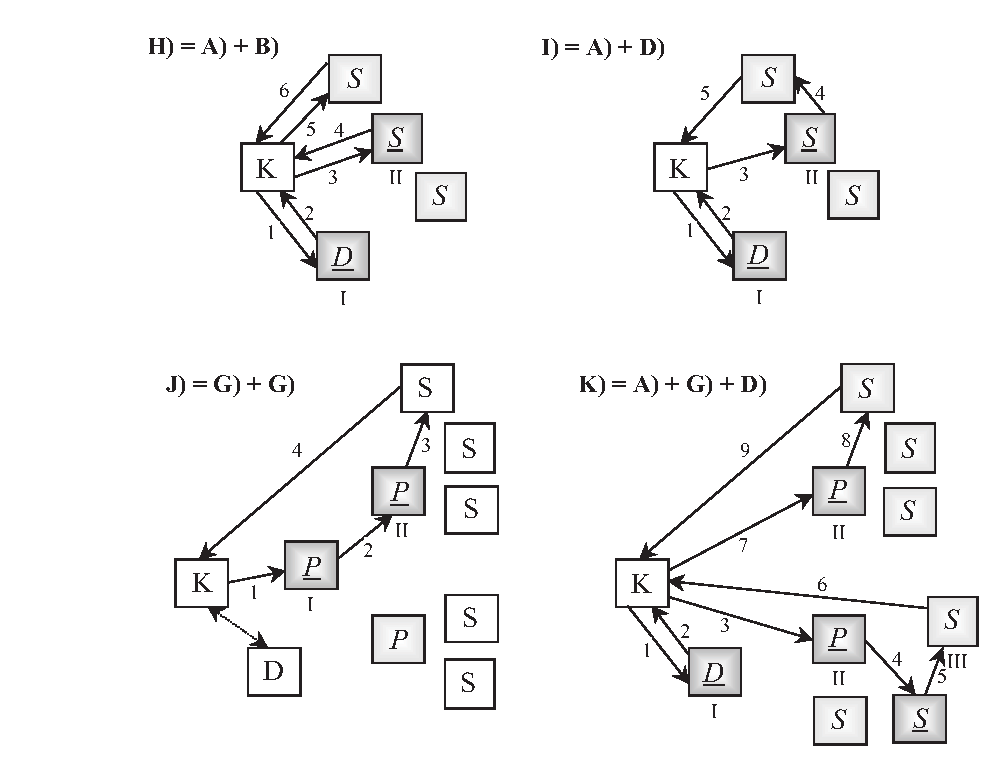
\includegraphics[width=4.9in]{./rysunki/complex_models.eps}
\caption{Z�o�one modele system�w do r�wnowa�enia obci��e�}
\label{complex_modele}
\end{figure}

\begin{itemize}
\item Systemy z szeregowaniem jednostopniowym. Systemy z szeregowaniem jednostopniowym odzwierciedlaj� modele: {\bf A, E, F, G} (rys.\ref{proste_modele}). 
W modelu {\bf A} egzekutor zintegrowany jest z serwerem DNS, natomiast w modelach{\bf E, F, G} rol� egzekutora pe�ni dystrybutor 
lub prze��cznik webowy.
\item Systemy z szeregowaniem dwustopniowym. Przyk�adowe systemy z szeregowaniem dwustopniowym obrazuj� modele {\bf H, I, J} (rys.\ref{complex_modele}).
W przypadku {\bf H} oraz {\bf I} \cite{modele2,modele10,modele23,modele3} na pierwszym stopniu wykorzystywany jest model {\bf A}, natomiast na drugim, odpowiednio 
model {\bf B} lub {\bf D}. W obu przypadkach na pierwszym stopniu egzekutor zintegrowany jest serwerem DNS, natomiast na drugim rol� 
egzekutora pe�ni ten z serwer�w webowych, kt�ry zosta� wytypowany na poziomie serwera DNS. Przypadek {\bf J} ukazuje kaskadowe 
z�o�enie modeli {\bf G} (rys.\ref{complex_modele}) w celu szeregowania ��da� w systemie rozproszonych klastr�w webowych \cite{NDUsersGuide}. Na obu stopniach rol� egzekutora 
mo�e pe�ni� dystrybutor lub prze��cznik webowy. Model ten charakteryzuje si� kr�tk� drog� zapyta�, jednak awaria pierwszego 
stopnia szeregowania unieruchamia ca�y system rozproszonych klastr�w.
\item Systemy z szeregowaniem tr�jstopniowym. Przyk�ad systemu z szeregowaniem tr�jstopniowym pokazuje model {\bf K} \cite{modele9}. Jest to 
system rozproszonych klastr�w webowych, gdzie ka�dy z serwer�w w klastrze ma wbudowany mechanizm szeregowania. Na pierwszym 
stopniu szeregowania wykorzystywany jest model {\bf A}, na drugim model {\bf G}, a na trzecim model {\bf B}, czyli na pierwszym stopniu 
egzekutor zintegrowany jest z serwerem DNS, na drugim role egzekutora pe�ni dystrybutor lub prze��cznik webowy, natomiast na 
trzecim ten serwer webowy, kt�ry zosta� wytypowany przez egzekutor na drugim stopniu. Ka�dorazowe zadzia�anie trzeciego 
stopnia szeregowania, mo�e powodowa� znaczne op�nienia, jednak model ten jest bardzo odporny na przeci��enia i awarie. 
\end{itemize}

\subsection{Podzia� ze wzgl�du na poziom szczeg�owo�ci szeregowania}

\subsubsection{Szeregowanie na poziomie serii ��da� o strony}
Aby zrealizowa� ��danie klienta o stron� umiejscowion� pod pewn� nazw� domenow�, mechanizm szeregowania, kt�ry jest 
zintegrowany z serwerem DNS, musi przydzieli� tej nazwie adres IP najlepszego serwera webowego (hostname resolution). Ze 
wzgl�du na du�� bezw�adno�� DNS kolejne ��dania klienta o strony umiejscowione pod t� nazw� domenow� b�d� przez pewien czas 
kierowane do tego samego serwera webowego. Przypadek, w kt�rym szeregowanie ��da� klient�w odbywa si� na poziomie serii ��da� 
o strony, przedstawia model {\bf A}. 

\subsubsection{Szeregowanie na poziomie ��dania o stron�}
W sk�ad strony webowej wchodzi zwykle wiele obiekt�w. Na tym poziomie przekierowanie ��dania o stron� poci�ga za sob� 
przekierowanie serii ��da� o jej elementy sk�adowe. Mechanizm szeregowania wykorzystuje w tym celu w�a�ciwo�ci protoko�u HTTP 
(HTTP redirection \cite{modele18}). Przypadki, w kt�rych wyst�puje tego typu szeregowanie, ukazuje model {\bf B} oraz {\bf E}. W przypadku modelu {\bf B}, gdy jeden 
z serwer�w webowych otrzymuje od klienta ��danie o stron�, je�li nie decyduje si� sam zrealizowa� zlecenia, 
odsy�a klientowi adres IP lub nazw� domenow� lepszego od siebie serwera \cite{modele23}. W przypadku modelu {\bf E}, gdy prze��cznik otrzymuje 
od klienta ��danie o stron�, odsy�a mu adres IP lub nazw� domenow� najlepszego serwera \cite{modele19}. 
Nale�y zaznaczy�, �e mo�e wyst�pi� tu zjawisko buforowania przez klienta adresu IP serwera, do kt�rego nast�pi�o 
przekierowanie. Mo�na w�wczas m�wi� o szeregowaniu na poziomie serii ��da� o strony.

\subsubsection{Szeregowanie na poziomie ��dania o obiekt}
Przypadki, w kt�rych szeregowanie odbywa si� na poziomie ��dania o obiekt, przedstawiaj� modele {\bf C, D, F} oraz {\bf G}. W tej grupie 
mechanizm szeregowania zajmuje si� przekierowywaniem pakiet�w (packet redirection). Pakiety zawieraj�ce ��danie o obiekt musz�
w komplecie trafi� do wybranego przez egzekutor serwera. Jednym ze sposob�w realizuj�cych ten cel jest zapisywanie wynik�w 
decyzji egzekutora w tzw. tablicy powi�za� (binding table).
Poniewa� w modelu {\bf D} ruch pakiet�w powracaj�cych (znacznie 
wi�kszy ni� w przypadku pakiet�w z ��daniami) jest kierowany do klienta z pomini�ciem serwera-egzekutora, model ten jest z 
powodzeniem implementowany. Charakterystyczn� cech� modeli {\bf F, G} jest to, �e egzekutor maskuje serwery webowe za pomoc� 
jednego, wirtualnego adresu IP-SVA (single virtual IP address). Aby przekaza� ��danie do konkretnego serwera, stosuje r�ne, 
niekiedy wyrafinowane techniki. Gdy egzekutor przekierowuje pakiety z ��daniami bez �wiadomo�ci ich tre�ci (content 
information blind), nazywany jest dystrybutorem (dispatcher, level 4 web-switch). Gdy egzekutor podczas podejmowania decyzji o 
przekierowaniu wykorzystuje informacj� zawart� w ��daniu (content information aware), nazywany jest prze��cznikiem webowym 
(content switch, level 7 web-switch).
Nale�y podkre�li�, �e niniejszy podzia� dotyczy wariantu, gdzie w modelach {\bf F, G} rol� egzekutora pe�ni dystrybutor. 
W przypadku gdy egzekutorem jest prze��cznik webowy, szeregowanie mo�e odbywa� si� na poziomie ��dania o obiekt, stron� oraz 
(dzi�ki umiej�tno�ci rozpoznawania znacznik�w cookie) serii ��da� o strony.

\subsection{Podzia� ze wzgl�du na poziom kontroli zapyta�}
Jest to podzia� wyodr�bniaj�cy modele, w kt�rych egzekutory maj� pe�na kontrol� nad zapytaniami kierowanymi do systemu 
serwer�w webowych.
\begin{itemize}
\item Pe�na kontrola zapyta�. Teoretycznie do tej grupy nale�� modele {\bf B, C, D, E, F} i {\bf G}. Klient, po otrzymaniu od 
serwera DNS adresu IP egzekutora, wszystkie zapytania kieruje tylko i wy��cznie do niego. W ten spos�b egzekutor ma 
stuprocentow� kontrol� nad zapytaniami. W rzeczywisto�ci sytuacja taka zachodzi w przypadku modeli {\bf F} oraz {\bf G}. Warto zwr�ci� 
uwag�, �e awaria lub zapchanie si� egzekutora powoduje unieruchomienie ca�ego systemu serwer�w webowych. 
\item Cz�ciowa kontrola zapyta�. Typowym przypadkiem, w kt�rym egzekutor sprawuje cz�ciow� kontrol� nad zapytaniami, jest 
model {\bf A}. Cz�ciowa kontrola wynika ze specyfiki funkcjonowania systemu DNS. R�wnie� modele {\bf B, E} nale�y zaliczy� do tej 
grupy ze wzgl�du na mo�liwo�� wyst�powania zjawiska buforowania przez klienta adresu IP serwera, do kt�rego nast�pi�o 
przekierowanie. Je�li modele {\bf C} i {\bf D} by�yby implementowane samodzielnie, egzekutor, kt�rego adres IP rozg�asza�by serwer 
DNS, sprawowa�by pe�n� kontrole nad zapytaniami. Jednak w przypadku modelu {\bf D} typowym rozwi�zaniem jest jego z�o�enie z 
modelem {\bf A} (model {\bf I} rys.\ref{complex_modele}). W takim przypadku ka�dy z egzekutor�w implementowanych w serwerach webowych sprawuje cz�ciow� 
kontrol� nad zapytaniami kierowanymi do systemu serwer�w webowych.
\end{itemize}

\subsection{Podzia� ze wzgl�du na poziom zaanga�owania egzekutora} 
Egzekutor mo�e by� w r�nym stopniu zaanga�owany w przekierowywanie zapyta� klienta. Mo�e by� r�wnie� zaanga�owany w proces 
przekazywania odpowiedzi. Rysuj� si� tu cztery grupy modeli: bierne, zwrotne, jednokierunkowe oraz dwukierunkowe:
\begin{itemize}
\item Model bierny. Jest to model {\bf A}, w kt�rym do egzekutora w og�le nie trafiaj� ��dania klienta o strony czy obiekty. 
Egzekutor odpowiada tylko na ��dania o prze�o�enie nazwy domenowej na adres IP najlepszego serwera (klastra) webowego, nie 
bior�c bezpo�redniego udzia�u w szeregowaniu zapyta� klienta.
\item Modele zwrotne. Nale�� do nich modele {\bf B, E} (rys.\ref{proste_modele}). Egzekutor, po otrzymaniu ��dania, zwraca klientowi adres IP lub nazw� 
domenow� najlepszego serwera, aby ten m�g� ponowi� ��danie. W modelu {\bf B} mo�e dodatkowo zapa�� decyzja o obs�u�eniu ��dania 
przez bie��cy serwer. Zaanga�owanie egzekutora w proces przekierowywania jest w tym przypadku minimalne.
\item Modele jednokierunkowe. Nale�� do nich modele {\bf D} oraz {\bf G}\cite{modele15,modele20,NDUsersGuide}. ��dania, kt�re osi�gaj� egzekutor, przekierowywane 
s� bezpo�rednio do serwer�w webowych. W modelu {\bf D} mo�e dodatkowo zapa�� decyzja o obs�u�eniu ��dania przez bie��cy serwer. 
Dzi�ki odpowiednim zabiegom technicznym serwery kieruj� odpowiedzi bezpo�rednio do klienta. Zaanga�owanie egzekutora w proces 
przekierowywania jest w tym przypadku �rednie.
\item Modele dwukierunkowe. Nale�� do nich modele {\bf C} i {\bf F} \cite{modele1,modele11,modele17} . Wszystkie ��dania, kt�re osi�gaj� egzekutor, 
przekierowywane s� bezpo�rednio do serwer�w webowych. W modelu {\bf D} mo�e dodatkowo zapa�� decyzja o obs�u�eniu ��dania przez 
bie��cy serwer. Serwery webowe wszystkie odpowiedzi przesy�aj� do egzekutora, kt�ry musi je przekierowywa� do klienta. 
\end{itemize}

\section{Witryny dynamiczne}

\hspace{0.63cm}Ju� nawet kilkudziesi�cioma dokumentami World Wide Web, czyli bardzo niewielkim serwisem, trudno jest zarz�dza�, 
zmienia� i dodawa� nowe fragmenty, czuwa� nad poprawno�ci� dost�pnych w nim danych. Z drugiej jednak strony oprogramowanie 
stosowane do korzystania z World Wide Web jest bardzo proste, szeroko znane i szybko uaktualniane.

Wi�kszo�� informacji zapisanych na komputerach i wykorzystywanych w biznesie czy przez �rodki przekazu zgromadzona jest w 
bazach danych, w tym najcze�ciej w relacyjnych bazach danych. Bazy danych pozwalaj� na kontrol� nad danymi, analizowanie ich, 
ogranizacj� i prezentacj� u�ytkownikowi w jak najbardziej prosty i skuteczny spos�b. Potrzebny jest jednak do nich dostep 
przez wyspecjalizowane oprogramowanie. W systemach klient/serwer jest to klient bazy danych; kolejny program, kt�ry musi 
poznawa� u�ytkownik, program nie zawsze prezentuj�cy najwy�szy poziom mo�liwo�ci technicznych czy �atwo�ci komunikacji z 
u�ytkownikiem.

Oba te systemy, World Wide Web i bazy danych, stworzone s� w tym samym celu -- efektywnego dost�pu do informacji. Ju� po kilku 
latach rozwoju World Wide Web zorientowano si�, �e mo�na je po��czy�, bior�c z ka�dego, co najlepsze. Po��czy� �atwo�� dost�pu,
jak� niesie przegl�darka World Wide Web z wysokim stopniem organizacji oferowanym przez relacyjn� baz� danych.

Sam serwer HTTP nie potrafi si� jednak bezpo�rednio porozumiewa� z baz�; potrzebuje dodatkowego oprogramowania. Dawniej 
najlepsz� metod� nawi�zania kontaktu mi�dzy serwerem HTTP a baz� by�o napisanie programu w standardzie CGI 
\footnote{ang. \emph{Common Gateway Interface}}. Program CGI przyjmuje informacje od serwera HTTP, przetwarza je i 
wysy�a do bazy danych, baza 
danych wykonuje zlecane jej zadanie, wysy�a efekt do programu CGI, kt�ry z kolei zwraca go przez serwer HTTP do klienta HTTP. 
Rezultatem jest najcz�ciej plik HTML. Dzi� mechanizm porozumiewania si� pozostaje taki sam, ale w miejsce programu CGI 
wchodzi program napisany w API serwera HTTP, na przyk�ad ISAPI dla Microsoft Internet Information Server. To drugie 
rozwi�zanie jest bardziej efektywne i pozwala na mniejsze obci��enie komputera, na kt�rym dzia�a serwer, ni� w przypadku 
u�ycia programu CGI.

Mo�na stworzy� serwis World Wide Web, kt�ry porozumiewa si� z baz� danych. Mo�na wpisywa� do bazy nowe informacje, na przyk�ad 
wype�niaj�c ankiet� marketingow�, mo�na przegl�da� istniej�ce informacje, poprawia� je o ile mamy do tego prawo a tak�e 
wyszukwia� potrzebne informacje.

Dok�adnie takie same mo�liwo�ci ma serwis wewn�trzny firmy -- intranetowy. Mo�e on s�u�y� do porozumiewania si� z firm� 
oddzia��w terenowych czy pracownik�w w podr�ach s�u�bowych, a tak�e do zwyk�ej, codziennej komunikacji z baz� danych. 
Przegl�darka World Wide Web jest �atwiejszym w obs�udze i bardziej znanym u�ytkownikom oprogramowaniem ni� specjalny klient 
bazy danych.

Do stworzenia takiego systemu potrzebny jest serwer HTTP i baza danych, a pomi�dzy nimi program po�rednicz�cy. Mo�na napisa� 
w�asne oprogramowanie po�rednicz�ce, ale r�wnie� skorzysta� z gotowych produkt�w.

\section{Testowanie serwer�w WWW}


Jak wiadomo s�aba wydajno�� wprost przek�ada si� 
na niezadowolenia klient�w, a niezadowolony klient opu�ci witryn� Web i
mo�e nigdy ju� na ni� nie wr�ci� \cite{savoia1,savoia2,savoia3}.

Przewidywanie jak witryna WWW b�dzie odpowiada� na specyficzne obci��enie
jest wielkim wyzwaniem. Od czasu jak sajty webowe stanowi� kompleksowe
systemy zawieraj�ce elementy sprz�towe, programowe i sieciowe pochodz�cymi od
r�nych producent�w, oraz posiadaj� bardzo r�ne profile wydajno�ciowe -- 
jest praktycznie niemo�liwa predykcja, jak dany system zachowa si� podczas
obci��enia. Jedynym pewnym sposobem sprawdzenia skalowalno�ci systemu
jest przeprowadzenie test�w wydajno�ciowych, w kt�rych nat�enie i 
charakterystyka przewidywanego ruchu jest symulowana tak realistycznie jak
to jest mo�liwe. 

Testowanie obci��enia witryn webowych stanowi priorytet dla firm robi�cych interesy online. Jak wielu u�ytkownik�w z 
akceptowalnymi czasami odpowiedzi mo�e obs�u�y� strona ? Jest to niezwykle wa�na informacja wykorzystywana do planowania 
kampanii reklamowych, estymacji bud�et�w bran�y IT a nawet do zwyk�ego dostarczania us�ug. I pomimo wagi tego problemu 
praktycznie wi�kszo�� test�w obci��eniowych jest wykonywana niepoprawnie, poniewa� nie odpowiadaj� one rzeczywistym warunkom. 

Poni�ej zostan� opisane elementy, niezb�dne podczas konstrukcji
wysoce realistycznych i dok�adnych test�w wydajno�ciowych sajt�w webowych (znajduj� si� r�wnie� najcz�ciej pope�niane w
typowych testach obci��eniowych b��dy oraz spos�b radzenia sobie z nimi):
\begin{enumerate}
\item Zrozumienie natury obci��enia

Pierwszym krokiem jest dok�adne i obiektywne zrozumienie
natury obci��enia, jakie musi zosta� wygenerowane, podczas symulacji ruchu na witrynie.

Niestety, testowanie obci��enia sajt�w webowych jest dziedzin� ralatywnie
now� (tote� s�abo zrozumian� i udokumentowan�), a do tego jest bardzo ezoteryczn�
dziedzin� test�w. �eby odpowiednio zrozumie� natur� obci��e� nale�y mo�liwie
cz�sto korzysta� z narz�dzia dokonuj�cego analizy log�w naszego web serwera.
Daje to mo�liwo�� obserwacji detali odwiedzin ka�dego u�ytkownika: jego adresu IP, daty i czasu odwiedzin; jakie, 
ile i o jakiej wielko�ci dane pobiera�, czy pobranie by�o zako�czone sukcesem, czy nie oraz inne dane o sesji u�ytkownika, 
jego systemie operacyjnym i narz�dziu z jakiego korzysta�. 

    \begin{description}
    \item[Sesja u�ytkownika -- niezb�dne informacje]\

Wi�kszo�� potrzebnych informacji jakie nale�y wyekstrahowa� podczas analizy log�w s� informacje zwi�zane z sesjami 
u�ytkownik�w\footnote{ang. \emph{user sessions}}. Testy obci��eniowe najbardziej zwi�zane s� w�a�nie z sesjami u�ytkownika. 
Sesj� u�ytkownika definiuje si� jako sekwencj� pobra� stron zwi�zan� z unikatowym (pojedynczym, identyfikowalnym) u�ytkownikiem.

Typowa witryna webowa jest wizytowana przez szerok� gam� u�ytkownik�w z szerok� gam� dzia�a�. Np. u�ytkownicy stron zwi�zanych 
z szeroko rozumianym e--commersem: niekt�rzy z nich przyszli poogl�da� (\emph{browse}), niekt�rzy kupi�, jeszcze inni 
sprawdzi� status
zam�wie�. Nawet je�li grupa klient�w dokonuje pojedynczego dzia�ania, takiego jak kupowanie ksi��ki, ka�dy z tej grupy mo�e to 
realizowa� na szereg sposob�w. Niekt�rzy b�d� porusza� si� ze strony na stron� bardzo szybko, raczej nie dbaj�c o dok�adne 
przeczytanie znajduj�cych si� tam informacji, inni przeciwnie -- poruszaj� si� powoli czytaj�c ka�d� stron� bardzo uwa�nie. 
Niekt�rzy b�d� wyszukiwa� czytaj�c fragmenty wielu ksi��ek zanim zdecyduj� si� na kupno jednej, inni skieruj� si� od razu do 
miejsca zam�wienia \emph{(purchase page)}.

Zrozumienie tej szerokiej gamy akcji, dzia�a� i zachowa� jest niezb�dne (krytyczne) dla zaprojektowania test�w obci��eniowych, 
poniewa� dobrze zaprojektowany test powinien odzwierciedla� zachowania u�ytkownik�w tak precyzyjnie jak to tylko mo�liwe. 
Najlepsz� metod� jest u�ywanie analizator�w log�w (podczas pracy witryny) oraz wydobycie kluczowej grupy zmiennych zachowania 
klient�w najcz�ciej spotykanych na danym sajcie, adekwatnych do ruchu webowego. Niekt�re ze zmiennych, na kt�re zawsze 
powinno zwr�ci� si� uwag� to:
	\begin{itemize}
	\item d�ugo�� trwania sesji (mierzona w stronach);
	\item czas trwania sesji (duration) (mierzona w minutach i sekundach);
	\item typ stron wizytowanych podczas trwania sesji (strona domowa, strona informacji o produkcjie, strona informacji o kartach 
	kredytowych).
	\end{itemize}

Naturalnie nie s� to wszystkie zmienne maj�ce wp�yw na charakterystyk� obci��eniow� sajtu -- opr�cz nich nale�y wybra� jeszcze 
jakie� zmienne kt�re o specyfice danej witryny decyduj�.

Tak� specyfik� mo�na zauwa�y� na przyk�adzie: siedmio--stronicowa sesja, kt�rej rezultatem jest zam�wienie artyku�u znacznie 
bardziej obci��a system ni� siedmiostronicowa sesja, kt�rej wynikiem jest tylko przegl�danie dokument�w. Przegl�danie 
dokument�w jest zwykle zwi�zane z dokumentami statycznymi, za� na sesj�, kt�rej efektem jest dokonanie zakupu artyku�u sk�ada 
si� ca�y szereg czynnik�w takich jak: przeszukiwanie bazy danych zasob�w witryny, u�ytkownika, transakcji kart kredytowych z 
weryfikacj� (osobne systemy), a tak�e wys�anie potwierdzaj�cego zam�wienie e--maila. Statystycznie rzecz bior�c pojedyncza 
sesja zakupu mo�e poch�on�� zasoby sajtu tak jak dwadzie�cia sesji statycznych \emph{(browsing)}. 

W podobny spos�b mo�na por�wna� zakupy dokonywane przez nowych i sta�ych klient�w. Nowy u�ytkownik potrzebuje dokona� 
rejestracji, potwierdzenia i weryfikacji swoich danych, za� sta�y ju� nie. Zwi�zane z baz� danych zak�adanie u�ytkownika mo�e 
by� r�wne obci��eniu generowanemu przez pi�ciu sta�ych u�ytkownik�w, dlatego trzeba wyr�ni� co najmniej dwa typy 
wykorzystania zasob�w przy realizacji zakup�w.

Gdy zostan� ju� zdeterminowane wszystkie zmienne zwi�zane z sesj� u�ytkownika -- nale�y nast�pnie znale�� (zwykle r�wnie� w 
logach) rang� i dystrybucj� warto�ci tych zmiennych np. procentowa (w ca�o�ci ��da�) ilo�� ��danych stron podczas sesji.  Do 
takich cel�w mo�na u�ywa� narz�dzi statystycznych takich jak: odchylenie standardowe, jednak�e najlepszym sposobem 
charakteryzowania wi�kszo�ci zmiennych webowych test�w obci��eniowych jest u�ycie rozproszenia jako warto�ci dyskretnej.

Wielko�� detali i precyzj� z jak� nale�y analizowa� te zmienne zale�y od struktury sajtu (i jej komplikacji), czasu test�w, 
oraz analizy wynik�w. 

    \item[Wsp�bie�ni u�ytkownicy]\

Zazwyczaj w testach obci��eniowych witryn webowych podaje si� warto�ci obci��enia 
spowodowanego naraz wsp�u�ytkuj�cymi zasoby u�ytkownikami. Jednak�e wsp�bie�ni u�ytkownicy nie powinni by� widziani 
jako zmienna wej�ciowa w te�cie, ale jako rezultat wielu r�nych czynnik�w. A zwkle podaje si� np. strona 
zosta�a przetestowana z obci��eniem 1000 wsp�bie�nymi u�ytkownikami. Liczba wsp�bie�nych u�ytkownik�w nie jest miernikiem 
obci��enia. Warto�� ta jest rezultatem wydajno�ci (zdolno�ci do przyj�cia obci��enia) witryny. Efektem pracy na wolniejszym 
sajcie b�dzie wi�ksza liczba wsp�bie�nych u�ytkownik�w. Mo�na to pokaza� na przyk�adzie -- je�li na stron� loguje si� trzech 
u�ytkownik�w w odst�pnie czasowym 1min i pracuj� po 1 min (np. dokonuj� zakup�w) -- to tylko i wy��cznie w zale�no�ci od 
wydajno�ci witryny oraz jej obci��enia b�dzie 0, 2 i 3 naraz pracuj�cych u�ytkownik�w. Zatem je�li wydajno�� witryny webowej z 
jakiego� powodu spada to wzrasta� b�dzie liczba wsp�bie�nych u�ytkownik�w. Trzeba jednak�e doda� jeszcze jeden element -- 
je�li wydajno�� sajtu spada (ro�nie liczba wsp�bie�nych u�ytkownik�w) ro�nie tak�e ilo�� u�ytkownik�w, kt�rzy rezygnuj� z 
korzystania z jego zasob�w. Je�li witryna jest bardzo szybka to mog� si� zdarzy� sytuacje, �e ilo�� wsp�bie�nych u�ytkownik�w 
b�dzie oscylowa� wok� zera (nawet przy ich du�ej ilo�ci). 

Z tych powod�w u�ywanie jako miernika obci��enia strony ilo�ci wsp�pracuj�cych naraz u�ytkownik�w jest (je�li ma by� 
realistyczne) bardzo trudne, a wyniki zawsze odbiegaj� od rzeczywistych. Znacznie lepszym wska�nikiem obci��enia witryny jest 
liczba sesji u�ytkownika wystartowana na godzin�. Ma to wa�n� zalet� -- jest to warto�� sta�a, niezmienna w zale�no�ci od 
wydajno�ci witryny w te�cie. Daje wska�nik ilu u�ytkownik�w otrzyma stron� pierwsz� witryny -- to czy ci u�ytkownicy uko�cz� 
swoj� sesj�, czy nie zale�y ju� od zdolno�ci strony do uniesienia danego obci��enia. I jest to w�a�nie ta warto��, kt�r� si� 
poszukuje podczas wykonywania test�w.

    \item[Rezygnacja klient�w]\

Kolejn� wa�n� wielko�ci�, niejednokrotnie �le szacowan� w testach, a maj�c� znaczny wp�yw na testy obci��eniowe 
witryny jest rezygnacja klient�w w trakcie sesji. U�ytkownicy cz�sto rezygnuj� podczas sesji np. zakup�w z powodu bardzo 
d�ugich odpowiedzi serwera. Zmienn� t� nale�y r�wnie� bra� pod uwag� podczas wykonywania test�w obci��eniowych na 
przygotowywanym 
sajcie. Symulacja porzucania przez u�ytkownik�w sesji powinna by� dokonana tak rzeczywi�cie jak to tylko mo�liwe. Je�li nie, 
podczas test�w b�dzie si� symulowa� obci��enie tak wielkie jakie mo�e nigdy nie nast�pi�, lub w�skie gard�a, kt�re w 
rzeczywisto�ci nigdy si� nie pojawi�. Pominie si� zatem najbardziej istotne wyniki test�w obci��eniowych: czyli 
u�ytkownik�w, kt�rzy mog� porzuci� sesj� z powodu s�abej wydajno�ci. Zatem testy stan� si� nieu�yteczne. W poni�szej 
tabelce znajduj� si� przyk�adowe zale�no�ci pomi�dzy liczb� opuszczaj�cych witryn� u�ytkownik�w, a czasem oczekiwania na 
okre�lon� stron�.
\begin{table}[h]
\centering
\begin{scriptsize}
\begin{tt}
\begin{tabular}{|c|c|c|c|c|}
\hline
{Typ strony}&{\% opuszczaj�cych}&{\% opuszczaj�cych}&{\% opuszczaj�cych}&{\% opuszczaj�cych}\\
{}&{ 0--5 s }&{ 5--10 s }&{ 10--15 s }&{ 10--20 s }\\
\hline\hline
{Strona domowa}&{0\%}&{30\%}&{45\%}&{75\%}\\
\hline
{Stock quote}&{0\%}&{15\%}&{25\%}&{45\%}\\
\hline
{Stock Transaction}&{0\%}&{0\%}&{0\%}&{15\%}\\
\hline
{Account Information}&{0\%}&{5\%}&{15\%}&{35\%}\\
\hline
\end{tabular}
\end{tt}
\caption{�redni stopie� porzucania witryny w \% dla r�nych typ�w stron}
\label{porzucanie}
\end{scriptsize}
\end{table}
Je�li zatem odpowied� oczekiwania na stron� domow� wynosi 5 sek. lub mniej nie obserwuje si� ucieczki klient�w. Jednak�e 
powy�ej tego czasu rezygnacja z oczekiwania staje si� coraz wyra�niejsza, by w czasie 15--20 sek. $3/4$ obecnych na witrynie 
klient�w ju� zrezygnowa�o. Jednak�e nale�y zwr�ci� uwag� na jeszcze jeden zwi�zany z tym szczeg�. Rezygnacja u�ytkownik�w 
zmniejsza obci��enie, zatem wydajno�� zaczyna si� zwi�ksza�, mniej u�ytkownik�w rezygnuje -- a� w ko�cu obci��enie z powrotem 
powoduje oczekiwania na realizacj� ��da� o strony i cykl si� powtarza. Jest to oczywi�cie przyk�ad. Rezygnacja u�ytkownik�w z 
us�ug witryny jest bardzo wa�n� zmienn� pokazuj�c�, �e dany sajt nie jest w stanie satysfakcjonuj�co zapewnia� us�ug przy 
obci��eniu. Najcz�ciej oprogramowanie do testowania potrafi symulowa� rezygnacj� u�ytkownik�w, ale z ekstremalnych powod�w -- 
zwykle 60--120sek. Jednak�e takie warto�ci s� nie do przyj�cia gdy� praktycznie nikt nie czeka tyle czasu. Aby m�c wykona� 
testy obci��eniowe tak prawdopodobne jak to tylko mo�liwe, mo�na skonfigurowa� testowan� witryn� w taki spos�b, aby 
przekierowywa� cz�� u�ytkownik�w na wolniejszy mirror tej witryny. Mo�na np. w ten spos�b: 90\% ruchu jest kierowane na 
zwyk�y serwer, za� 10\% na wolniejszy mirror, na kt�rym np. strona domowa b�dzie serwowana p�niej o 5 sek. W takiej 
konfiguracji nale�y ten dwuserwerowy system uruchomi� na kilka godzin lub dni, do czasu otrzymania znacz�cych wynik�w. Po tym 
czasie nale�y dokona� analizy porzucaj�cych transakcje webowe klient�w. Je�li na zwyk�ym serwerze opuszczanie sesji po stronie 
domowej si�ga 6\%, za� na tym wolniejszym 20\%, trzeba si� liczy� z opuszczaniem witryny przez 14\% klient�w, kt�rzy nie b�d� 
zbyt cierpliwi by poczeka� kolejne 5 sek.

Porzucanie operacji webowych przez klient�w nie jest interesuj�cym wynikiem, samym w sobie -- daje pogl�d na to jakie cz�ci 
sajtu s� najbardziej obci��one w warunkach pracy. Je�li np. strona domowa jest wyj�tkowo wolna, wi�kszo�� u�ytkownik�w nawet 
nie rozpocznie sesji. Wida� zatem, �e odpowiednie symulowanie tego parametru jest bardzo istotne dla stworzenia wydajnego 
sajtu.

    \item[Dystrybucja zapyta� o stron�]\

Kolejn� wa�n� zmienn�, kt�rej warto po�wi�� uwag� jest dystrybucja zapyta� o  stron�. Ta wa�na warto�� okre�la o jakie strony 
s� zapytania i w jakich proporcjach. Procedura zbierania tej danej jest dwustopniowa: najpierw nale�y zdefiniowa� 
skategoryzowane grupy stron, a nast�pnie obliczy� udzia� procentowy ��da� o strony w ka�dej grupie. 

    \end{description}

\item Estymacja wzrostu ruchu na witrynie

Kolejnym krokiem przy projektowaniu test�w obci��eniowych jest zrozumienie pewnych kluczowych zmiennych -- niezb�dnych do 
estymowania docelowego poziomu obci��enia:
    \begin{itemize}
    \item jak wzrasta ca�kowite obci��enie ruchu na sajcie;
    \item jaki jest poziom obci��enia pojedynczych pik�w, maj�cych wp�yw w ca�kowitym obci��eniu;
    \item jak szybko liczba u�ytkownik�w mo�e wp�yn�� na osi�gni�cie maksimum piku obci��eniowego;
    \item jak d�ugo trwaj� poszczeg�lne piki.
    \end{itemize}

Przy pomiarze poziomu obci��enia mo�na u�ywa� zmiennej: liczba sesji u�ytkownik�w na jednostk� czasu. Taki wyb�r wynika z jego 
prostoty w zrozumieniu i �atwo�ci analizy.

    \begin{description}
    \item[Estymacja przysz�ego ruchu webowego]\

Ocena szybko�ci wzrostu ca�kowitego obci��enia ruchu jest istotna, poniewa� rozmiar poziomu pik�w jest 
proporcjonalny do amplitudy ca�kowitego ruchu. Je�li ca�kowity ruch wynosi np. 100000 sesji na tydzie�, oznacza to piki o 
wielko�ci 1500 sesji na godzin�, zatem przy obci��eniu rz�du 200000 sesji na tydzie� piki (chwilowe obci��enia) mog� si�ga� 
3000 sesji na godzin�. 

Ca�kowity wzrost wielko�ci ruchu wynika z dw�ch czynnik�w: danych historycznych (o wzro�cie) oraz szacunk�w 
sprzeda�y/marketingu. Aby estymowa� te warto�ci, nale�y dokona� analizy tygodniowego ruchu oraz dowiedzie� si� od odpowiednich 
ludzi w firmie jak mo�e si� zmienia� ruch z miesi�ca na miesi�c, oraz jak mo�e wygl�da� zainteresowanie na witrynie po 
specjalnych ofertach marketingowych. Z takich informacji mo�na oszacowa� warto�� obci��enia w czasie -- czyli przysz�e 
mo�liwo�ci sajtu. 

    \item[Estymacja ruchu chwilowego]\

Po dokonaniu analizy wzrostu ca�kowitego obci��enia, nale�y estymowa� poziom nat�enia ruchu chwilowego. Jest to niezb�dne 
poniewa� ruch webowy jest raczej nier�wnomierny, a wiele sajt�w do�wiadcza znacz�cych chwilowych obci��e�. Zwykle zdarza si� 
to tylko kilka razy (raz, lub dwa w tygodniu lub kilka godzin dziennie). Gdy ruch webowy jest najwy�szy. Przyk�adem s� witryny 
pogodowe, na kt�rych nasilenie ruchu odbywa si� w pi�tek i sobot�, poniewa� u�ytkownicy potrzebuj� danych pogodowych z powodu 
plan�w weekendowych. Natomiast (trading) handel sieciowy zwykle do�wiadcza najwi�kszych obci��e� w okolicach czasu otwarcia i 
zamkni�cia sklepu. 

    \item[Szacowanie przebiegu ruchu chwilowego]\

Estymowanie jak szybko osi�gane jest docelowe chwilowe obci��enie, oraz przez jak d�ugi czas jest utrzymywane jest tak wa�ne 
jak estymacja amplitudy chwilowych obci��e�. Mo�na to pokaza� na przyk�adach:

Sprzeda� online (stock) do�wiadcza zwykle ekstremalnie ostrych chwilowych nat�e� ruchu (pik�w) w r�nym czasie jak np. 
otwarcie sklepu. W ci�gu kilku minut witryna przechodzi od nie przyjmowania zg�osze� po przyjmowanie ich tysi�cy naraz. Test 
obci��eniowy powinien dla tego typu sajt�w generowa� tak specyficzne wysokie chwilowe obci��enia zwykle w czasie od pi�ciu do 
dziesi�ciu minut. 

Sprzeda� ubra� online, mo�e do�wiadcza� innej charakterystyki obci��eniowej. Tutaj testy obci��eniowe powinny generowa� wzrost 
obci��enia (do docelowego maksymalnego) w czasie rz�du jedna dwie godziny. Szybszy wzrost mo�e odbiega� od sytuacji 
rzeczywistej. 

Czas trwania pik�w obci��eniowych jest r�wnie� bardzo wa�ny -- witryna radz�ca sobie z wysokim obci��eniem trwaj�cym pi�� do 
dziesi�ciu minut mo�e si� zupe�nie za�ama� podczas d�u�ej trwaj�cego wysokiego ruchu. 
    \end{description}

\item Dokumentowanie i projekt

Gdy wszystkie powy�ej wymienione informacje zostan� zebrane mo�na zaprojektowa� odpowiedni do danych warunk�w test 
obci��eniowy.

Kluczowymi elementami takiego testu s�:
    \begin{itemize}
    \item cele testu: zdeterminowanie jakiemu obci��eniu oraz w jaki spos�b b�dzie poddawana witryna, a tak�e czy wraz z 
    wzrastaj�cym ruchem jest w stanie mu podo�a�;
    \item kryteria jakie b�d� spe�nione podczas trwania klienckiego ��dania -- tzn. np. maksymalny czas oczekiwania na stron� lub 
    nawet czas po jakim ��danie mo�e zosta� odrzucone;
    \item opis skrypt�w testowych i ich typy: np. scrypt opisuj�cy tr�jstronicowe ��danie (strona domowa >> informacja o produkcie 
    >> zamowienie) oraz procentowe wykorzystanie tych typ�w skrypt�w;
    \item opis scenariusza czyli u�ycie skrypt�w testowych, czas ich uruchamiania oraz ich udzia� procentowy w ca�o�ci testu, a 
    tak�e czas i szybko�� narastania obci��enia (piki obci��eniowe).
    \end{itemize}
\end{enumerate}

\chapter{Zarz�dzanie wielokomputerowym serwisem WWW}
\label{r04}
W rozdziale tym znajdzie si� pr�ba odpowiedzi na pytanie co to jest kiedy i po co stosuje si� zarz�dzanie serwerem 
WWW (jakie s� parametry charakterystyczne oceny wydajno�ci i dost�pno�ci). Nast�pnie zostanie przedstawiona szczeg�owa 
taksonomia serwer�w WWW. Ostatnim punktem tego rozdzia�u 
b�dzie por�wnanie us�ug zapewnianych przez witryny statyczne i dynamiczne, opis zastosowa� i mo�liwo�ci obu 
typ�w tworzenia witryn oraz wymagania stawiane systemom WWW wraz z pogl�dowym przyk�adem.

\section{Wprowadzenie}

Jak zauwa�ono wcze�niej -- przysz�o�� serwis�w WWW nale�y do platform wieloserwerowych. Wynika to z mo�liwo�ci 
teoretycznie niograniczonej rozbudowy wraz ze wzrostem liczby u�ytkownik�w oraz ich wymaga�. Kolejn� zalet� jest 
r�wnie� spe�nianie bezpiecze�stwa przez takie wielokomputerowe systemy -- w dowolnym elemencie takiego systemu -- nodzie --
mo�e nast�pi� praktycznie dowolnego rodzaju uszkodzenie -- tak dysk, jak pami�� operacyjna czy procesor -- wtedy poszczeg�lne
procesy s� transportowane na inne nody, nawet w przypadku uszkodzenia jednej maszyny, nie spowoduje to przestoju. Jednak�e aby
taki system spe�nia� dobrze swoje zadania potrzebne jest oprogramowanie lub urz�dzenie pozwaj�ce nim zarz�dza� czyli 
odpowiednio rozdysponowa� ��dania klienckie oraz wykrywa� uszkodzenia poszczeg�lnych element�w uk�adu. W literaturze
przyj�o si� takie rozdysponowanie zapyta� pomi�dzy poszczeg�lne nody nazywa� r�wnowa�eniem obci��enia systemu\footnote{ang. 
\emph{load balancing, LB}}. 

\section{R�wnowa�enie obci��enia -- metody}

R�wnowa�enie obci��e� (ang. \emph{load balancing}) w systemach rozproszonych, to zagadnienie z dziedziny 
rozdzia�u zada� polegaj�ce na dystrybucji pomi�dzy w�z�y systemu nap�ywaj�cych do niego zlece� tak, aby  
maksymalizowa� jego ��czn� wydajno��. Oznacza to, �e dzia�alno�� zwi�zana z rozdzia�em zada� nie mo�e powodowa� 
obci��enia systemu w stopniu, kt�ry niwelowa�by korzy�ci wynikaj�ce z faktu zr�wnowa�enia obci��e� jego w�z��w. 
Angielski termin load balancing w rzeczywisto�ci funkcjonuje jako reprezentant tej problematyki, gdy� traktowany 
�ci�le oznacza doprowadzenie systemu rozproszonego do stanu w kt�rym wszystkie jego w�z�y obci��one s� w 
dok�adnie r�wnym stopniu, nawet je�eli oznacza�oby to odebranie zada� jednemu z nich. W stosunku do wi�kszo�ci 
rozwi�za� przemys�owych z tego zakresu nale�a�oby poprawnie u�ywa� okre�lenia wsp�dzielenie obci��e� (ang. \emph{
load sharing}) lub bardziej og�lnie, rozdzia� obci��e� (ang load distribution). Realizacja �cis�ego r�wnowa�enia 
obci��e� wi��e si� z konieczno�ci� implementacji metod odbierania zada� w�z�om, powoduje to wzrost z�o�ono�ci 
realizacji algorytmu, a sam proces odbierania zadania jest do�� kosztowny. Wzrost wydajno�ci uzyskiwany dzi�ki 
idealnemu zr�wnowa�eniu obci��e� w systemie w por�wnaniu do wydajno�ci uzyskiwanej przy zastosowaniu 
wsp�dzielenia obci��e� nie jest zwykle na tyle du�y, by usprawiedliwia� ponoszenie koszt�w zwi�zanych z 
pokonaniem z�o�ono�ci realizacji �cis�ego r�wnowa�enia obci��e� \cite{barylo13,barylo16,barylo17}. W tej pracy, tak jak w 
literaturze angielskoj�zycznej, u�ywany jest termin r�wnowa�enie obci��e�, chyba �e zaznaczono inaczej.
Wydaje si�, �e najskuteczniejsz� metod� zwi�kszenia wydajno�ci serwera WWW jest powielenie (lub podzia�) danych, kt�re 
serwer 
udost�pnia, pomi�dzy grup� po��czonych sieci� komputer�w (dodatkowych serwer�w WWW) i zapewnienie dost�pu do 
tej grupy tak jak do pojedynczego serwera z uwzgl�dnieniem transparentnego dla u�ytkownika i maksymalizuj�cego 
wydajno�� podzia�u ��da� HTTP pomi�dzy poszczeg�lne elementy grupy. Taka grupa nazywana klastrem lub farm� 
serwer�w stanowi swoisty system rozproszony, kt�rego wydajno�� mo�na maksymalizowa� stosuj�c r�wnowa�enie 
obci��e�. Nale�y zaznaczy�, �e chocia� termin klaster oznacza serwery po��czone w ca�o�� logiczn� (dost�pne pod 
jedn� nazw� lub adresem IP), nie implikuj�c �adnych ogranicze� na geograficzne rozproszenie serwer�w, to wiele 
rozwi�za� komercyjnych wymaga, by serwery nale��ce do klastra znajdowa�y si� w obszarze jednej sieci lokalnej 
(mia�y jednakow� cz�� globaln� adresu IP).

\section{Przegl�d i podzia� webowych algorytm�w szeregowania}

Wszystkie mechanizmy realizuj�ce zarz�dzanie dost�pem do rozproszonych serwer�w WWW musz� mie� zaimplementowany konkretny 
algorytm, na podstawie kt�rego b�d� mog�y podejmowa� decyzj� o przes�aniu zapytania do najlepszego serwera. W zale�no�ci od 
stopnia skomplikowania systemu i mo�liwo�ci implementacyjnych wykorzystywane algorytmy mog� mie� r�n� z�o�ono�� obliczeniow�. 
Zastosowane strategie zale�ne s� r�wnie� od informacji, jakie posiada system na temat ilo�ci zapyta� generowanych przez 
klient�w oraz informacji o stanie serwer�w wchodz�cych w sk�ad rozproszonego systemu WWW. Mo�na je podzieli� na kilka 
kategorii w zale�no�ci od ilo�ci informacji, jaka wykorzystywana jest przy podejmowaniu decyzji. 

\subsection{Algorytmy statyczne (nie wykorzystuj�ce informacji zewn�trznych)}
Je�eli w procesie szeregowania nie s� wykorzystywane �adne informacje o stanie serwer�w lub strumieniu zapyta�, m�wi si� o 
algorytmach statycznych. Te mechanizmy, to najprostsze rozwi�zania gwarantuj�ce w niewielkim stopniu roz�o�enie obci��enia 
pomi�dzy serwery. Rozk�ad ten jest bardzo przypadkowy i nie gwarantuje r�wnomiernego wykorzystania zasob�w ani wysokiej 
dost�pno�ci systemu, jednak�e s� one najszybszymi, gdy� wymagaj� najmniej mocy obliczeniowej. Do takich algorytm�w nale��:
\begin{itemize}
\item Random -- system nie posiada �adnych informacji o stanie serwer�w WWW, jak r�wnie� nie posiada informacji o tym, do 
kt�rego serwera ostatnio skierowane zosta�o zapytanie;
\item Round--robin -- system nie posiada �adnych informacji o stanie serwer�w WWW, posiada jednak informacj� historyczn� o tym, 
do kt�rego serwera skierowane zosta�o ostatnio nades�ane zapytanie.
\end{itemize}

\subsection{Algorytmy dynamiczne (wykorzystuj�ce informacj� zewn�trzn�)}
W procesie szeregowania mo�na stosowa� bardziej rozbudowane mechanizmy zarz�dzania. Aby zwi�kszy� efektywno�� szeregowania, 
mo�na stosowa� strategie wykorzystuj�ce informacje o kliencie. Wyb�r najlepszego serwera mo�e odbywa� si� na podstawie adresu 
IP lub numer portu TCP wykorzystywanego przez klienta. Mo�liwe jest r�wnie� wykorzystywanie tzw. alarm�w generowanych przez 
serwery. Do mechanizmu decyduj�cego o wyborze serwera w okre�lonych odst�pach czasowych przekazywana jest informacja zwrotna o 
obci��eniu serwera lub informacja o przekroczeniu jakiego� okre�lonego parametru. Szeregowanie mo�e odbywa� si� na podstawie 
jednej z metryk okre�laj�cych obci��enie:
\begin{itemize}
\item ilo�ci aktywnych po��cze� z serwerem,
\item wykorzystania dysku i/lub procesora serwera,
\item przewidywanego strumienia zapyta� w okre�lonym czasie.
\end{itemize}

W przypadku modeli, gdzie mechanizmy szeregowania w ca�o�ci kontroluj� strumie� zapyta�, mog� by� stosowane algorytmy 
dystrybuuj�ce zapytania w zale�no�ci od wielko�ci nap�ywaj�cego strumienia oraz obci��enia serwer�w obs�uguj�cych te 
zapytania. Dzi�ki informacjom zbieranym od serwer�w mo�liwe jest szacowanie parametr�w maj�cych wp�yw na szybko�� ich 
odpowiedzi. Mog� to by�:
\begin{itemize}
\item ilo�� zapyta� zrealizowana w okre�lonym czasie,
\item obci��enie procesora w danym momencie,
\item poziom wykorzystania dysk�w w serwerze.
\end{itemize}
Takie rozwi�zania umo�liwiaj� wyeliminowanie przeci��onych serwer�w. W znacznym stopniu zwi�ksza to dost�pno�� klient�w do 
danych oraz wp�ywa na lepsze wykorzystanie zasob�w. 

Algorytmy dynamiczne mo�emy w zale�no�ci od miejsca analizy podzieli� na:
\begin{itemize}
\item \emph{Server Info Aware} -- czyli wykorzystuj�ce informacje o stanie serwera;
\item \emph{Client Info Aware} -- czyli wykorzystuj�ce specyfik� ��da� klienckich -- przekierowuj�ce ��dania w zale�no�ci
od typu zapytania klienckiego (dane z serwera baz danych, wykorzystuj�ce skrypty CGI, zawieraj�ce pliki multimedialne itp.)
\end{itemize}

\subsection{Algorytmy szeregowania wykorzystywane po stronie serwera DNS}

\subsubsection{Algorytmy nie wykorzystuj�ce informacji o stanie systemu -- statyczne}

\begin{itemize}
\item Round--robin DNS\\
Podej�cie to zosta�o zastosowane jako pierwsze przy budowie skalowalnego systemu serwer�w webowych przez NCSA \cite{modele22}. Kod 
serwera DNS (np. Unixowy BIND) bez �adnych modyfikacji mo�e wykorzystywa� algorytm Round--robin. Obci��enie serwer�w nie jest 
zbyt dobrze 
r�wnowa�one ze wzgl�du na mechanizm cache dla powi�za� nazwa domenowa - adres IP. Stosuj�c takie podej�cie, nie ma si� r�wnie� 
kontroli nad dost�pno�ci� serwer�w oraz nie uwzgl�dnia si� mo�liwo�ci zastosowania serwer�w o r�nej wydajno�ci.
Jest to algorytm bardzo prosty zar�wno w dzia�aniu jak i implementacji (w stadardowym serwerze DNS mo�na go zastosowa�, bez
konieczno�ci modyfikacji kodu serwera). Jego dzia�anie polega na cyklicznym rozsy�aniu pakiet�w do kolejnego na li�cie serwera.
Oczywi�cie najlepsze wyniki osi�ga si� dla komputer�w symetrycznych sprz�towo. Modyfikacj� tego algorytmu jest 
Weighted Round--Robin, w kt�rym to algorytmie mo�na statycznie nada� wagi poszczeg�lnym serwerom w zale�no�ci od ich 
wydolno�ci;
\item Random\\
\end{itemize}

\subsubsection{Algorytmy wykorzystuj�ce informacje o stanie systemu}

Alternatyw� dla algorytmu Round--robin najcz�ciej stosowanego w przypadku serwera DNS s� algorytmy wykorzystuj�ce informacje o 
stanie systemu (wielko�ci przewidywanego strumienia zapyta�, aktualnego obci��enia serwer�w). Okazuje si�, �e regu�y bazuj�ce 
wy��cznie na stanie obci��enia serwer�w WWW s� nieefektywne. W rzeczywisto�ci, w zwi�zku z hierarchicznym buforowaniem danych 
przez serwery DNS, pojedyncze zapytanie od klienta mo�e spowodowa� nap�yw wielu innych zapyta�. Wynika z tego, �e informacja o 
aktualnym obci��eniu nie jest w �aden spos�b zwi�zana z przysz�ym obci��eniem \cite{ModeleFunkcjonalne}.
Podej�cie pozwalaj�ce oszacowa� nadchodz�cy strumie� zapyta� (\emph{hidden load weight}) w czasie TTL (\emph{Time To Live}) jest najbardziej 
efektywne. Dzi�ki tym informacjom mo�na przypisa� r�ne warto�ci TTL dla r�nych domen i estymowa� wielko�� ukrytego, czyli 
niekontrolowanego przez serwer DNS strumienia zapyta�. Przyk�adami tego typu algorytm�w s� \cite{modele14}:
\begin{itemize}
\item Multi tie round--robin -- dla ka�dej domeny lub ich okre�lonych zbior�w przypisywane s� r�ne warto�ci TTL, pozwalaj�ce na
zr�wnowa�enie strumieni zapyta� do ka�dego serwera WWW.
\item Dynamically accumulated load (DAL) -- rozbudowana wersja algorytmu Multi tie Round--robin polegaj�ca na zbieraniu 
informacji o estymowanej wielko�ci obci��enia serwer�w i zmianie �a�cucha przypisa� adres�w w serwerze DNS w zale�no�ci od 
zak�adanego obci��enia.
\item Minimum residual load -- modyfikacja algorytmu DAL polegaj�ca na estymowaniu wielko�ci ukrytego obci��enia i warto�ci TTL.
Po up�ywie TTL serwer WWW odpytywany jest o rzeczywist� wielko�� strumienia zapyta�, jaka zosta�a do niego skierowana. Dzi�ki 
temu algorytm ma informacj� o stanie serwera. Powoduje to r�wnie� zmian� kolejno�ci przypisa� w serwerze DNS;
\end{itemize}

\subsubsection{Algorytmy adaptacyjne}

Algorytmy r�wnowa�enia bazuj�ce na oszacowaniu hidden load weight oraz alarmach z krytycznie przeci��onych serwer�w pozwalaj� 
na du�o bardziej efektywne, w por�wnaniu z algorytmami Round--robin, r�wnowa�enie serwer�w WWW. Niestety, s� one efektywne 
tylko w przypadku rozproszenia serwer�w homogenicznych. Inn� grup� algorytm�w przeznaczonych do r�wnowa�enia obci��enia 
serwer�w heterogenicznych s� algorytmy adaptacyjne. W przypadku algorytm�w adaptacyjnych warto�� TTL przypisywana jest 
dynamicznie do ka�dego ��dania na podstawie przewidywanego hidden load weight oraz wydajno�ci serwera, do kt�rego zapytanie 
zosta�o przypisane. Idea tego podej�cia polega na uwzgl�dnieniu pewnej warto�ci $\xi_i$ opisuj�cej moc obliczeniow� serwera $S_i$. 

Algorytmy te podzielone zosta�y na dwie grupy \cite{modele25}:
\begin{itemize}
\item probabilistyczne -- realizacja metody bazuje na algorytmie Round--robin. Za ka�dym razem losowo generujemy liczb� 
$\gamma(0\leq\gamma\leq1)$. Je�eli zapytania przypisane s� aktualnie do serwera $S_i$, to jako nast�pny zostanie 
wybrany $S_{i+1}$ tylko wtedy,
gdy $\gamma\leq\xi_i$, w przeciwnym przypadku warunek zostaje rozpatrzony dla kolejnego serwera. 
Warto�� TTL oblicza si� ze wzoru:
\begin{equation}
TTL_i = \frac{\eta}{\xi_i}
\end{equation}
\item deterministyczne -- ide� algorytmu jest takie dostosowanie czasu TTL, aby bardziej wydajne serwery obs�ugiwa�y wi�cej 
zapyta�, a mniej wydajne nie by�y przeci��ane. Dla ka�dej domeny $i$ obs�ugiwanej przez system serwer�w webowych zostaje 
przypisana warto�� TTL z  uwzgl�dnieniem wydajno�ci serwera $j$ wed�ug wzoru:
\begin{equation}
TTL_{ij} = \frac{\eta * c_i}{\xi_i}
\end{equation}
gdzie $\eta$ jest warto�ci� sta��, zale�n� od liczby zdefiniowanych domen generuj�cych zapytania.
\end{itemize}

\subsection{Algorytmy szeregowania wykorzystywane w dystrybutorach}

Stosowane tutaj algorytmy  \cite{modele13} s� najprostsze, poniewa� dystrybutor obs�uguje wszystkie nadchodz�ce pakiety i konieczne jest 
zminimalizowanie czasu po�wi�canego na ich obs�ug�. Rekompensat� za konieczno�� obs�ugi wszystkich pakiet�w jest pe�na 
kontrola nap�ywaj�cego strumienia zapyta�. Stosowane w tym przypadku algorytmy mo�na podzieli� na trzy podstawowe grupy:
\begin{itemize}
\item Information less -- nie wykorzystuj�ce �adnych informacji o stanie systemu,
\item Client info aware -- wykorzystuj�ce informacje o adresie IP klienta lub numerze portu, przez kt�ry komunikuje si� z 
serwerem,
\item Server state aware -- wykorzystuj�ce informacje o stanie serwera, do kt�rego przekazuj� zapytanie.
\end{itemize}

Tak jak w przypadku algorytm�w stosowanych w serwerze DNS, najmniej efektywne s� algorytmy nie wykorzystuj�ce �adnych 
dodatkowych informacji, czyli Random i Round--robin.

Wykorzystuj�c informacje o kliencie, np. jego adres IP, mo�na zastosowa� bardziej efektywne rozwi�zania. Przyk�adem takiego 
algorytmu jest Client partition.

W zwi�zku z zarz�dzaniem strumieniem zapyta� na poziomie pakiet�w, odwo�ania nadchodz�ce z tego samego adresu, dotycz�ce 
pojedynczej sesji, musz� by� przekierowywane do tego samego serwera. Dopiero ��dania nowego obiektu mog� by� przes�ane na inny 
serwer. Wymaga to utrzymywania w systemie tablicy aktywnych po��cze�. Dzi�ki temu mo�na oszacowa�, kt�ry z serwer�w obci��ony 
b�dzie dodatkowymi zapytaniami w najbli�szym czasie i na tej podstawie wybra� najlepszy, do kt�rego skierowane zostanie 
kolejne zapytanie. Realizowane jest to na podstawie algorytmu Least loaded server. 
\begin{figure}[h]
\centering
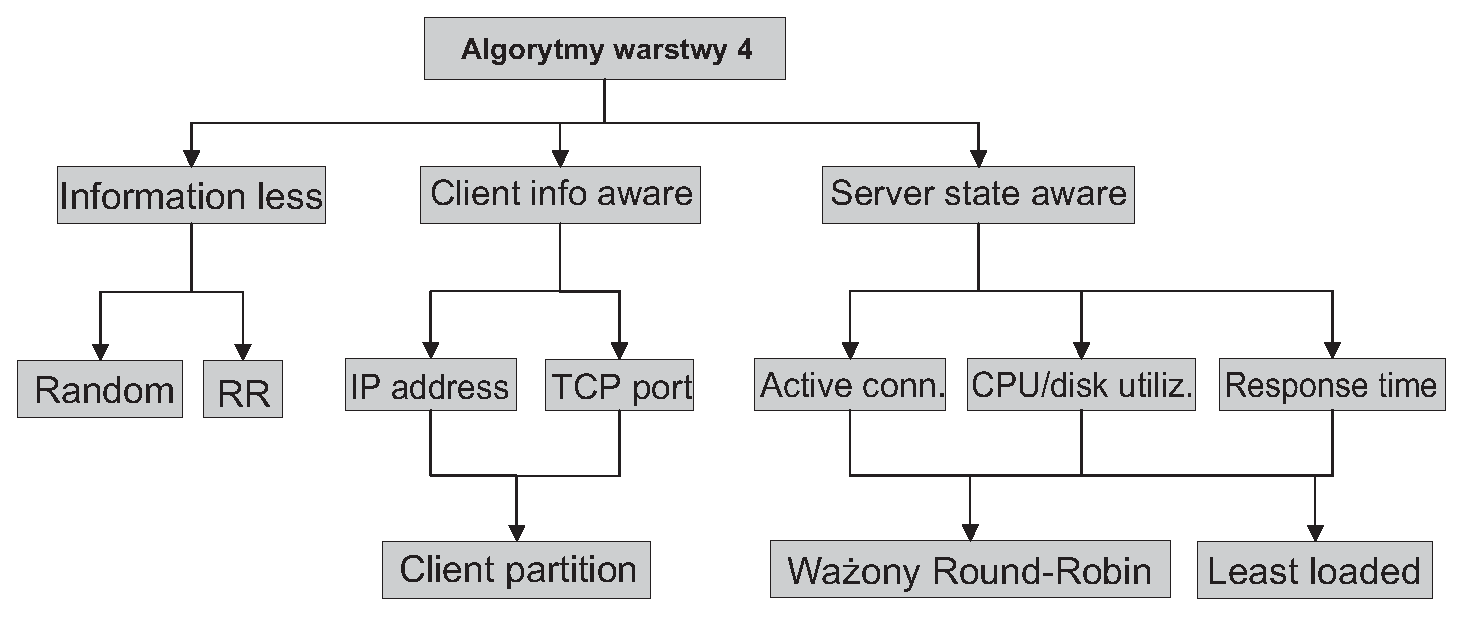
\includegraphics[width=4.9in]{./rysunki/level_4_alg.eps}
\caption{Algorytmy stosowane w dystrybutorach.}
\label{level_4_alg}
\end{figure}

Opr�cz informacji o tym, kto przesy�a zapytania do systemu webowego, mo�na r�wnie� uzyska� dane na temat pracy poszczeg�lnych 
serwer�w w systemie. Aby poprawi� jako�� szeregowania zapyta�, w algorytmie dokonuj�cym wyboru najlepszego serwera stosuje si� 
r�nego rodzaju metryki okre�laj�ce aktualne obci��enie serwer�w. Najcz�ciej stosowanymi algorytmami w tym przypadku s� Least 
loaded server oraz Weighted Round--robin. 
\begin{itemize}
\item W przypadku algorytmu Least loaded server dzi�ki wybranemu kryterium (okre�lonej metryce) wiemy, kt�ry z serwer�w 
powinien przyj�� kolejne zapytanie. Odbywa si� to na zasadzie: najmniej obci��ony serwer przyjmuje kolejne zlecenie. 
\item Stosuj�c algorytm Weighted Round--robin, przy wyborze kolejnego serwera mo�na uwzgl�dnia� metryk� jako parametr funkcji 
wyboru najlepszego serwera.

Wa�nym wi�c elementem funkcjonowania tego rozwi�zania jest dob�r metryki b�d�cej powy�szym parametrem. Istnieje 
mo�liwo�� kontrolowania nast�puj�cych parametr�w:
\begin{itemize}
\item input metric -- informacja pozyskiwana jest przez dystrybutor bez wsp�prcy z serwerami, np. liczba aktywnych po��cze� 
miedzy dystrybutorem a poszczeg�lnymi serwerami,
\item server metric -- informacja pozyskiwana jest przez serwery i dostarczana dystrybutorowi, np. wykorzystanie procesora lub 
dysku, czas miedzy otrzymaniem zapytania a wys�aniem odpowiedzi,
\item forward metric -- informacja pozyskiwana jest bezpo�rednio przez dystrybutor, np. emulacja zapyta� do serwer�w webowych.
\end{itemize}
\end{itemize}

\subsection{Algorytmy szeregowania wykorzystywane w prze��cznikach webowych}
Prze��czniki webowe maj� r�wnie� mo�liwo�� kontrolowania 100\% ruchu do serwer�w. Zatem i tu konieczne jest wykorzystanie jak 
najprostszych mechanizm�w zarz�dzania. W przypadku prostych rozwi�za� wystarczaj�co wydajne s� algorytmy statyczne. Sytuacja 
taka wyst�puje, gdy czasy realizacji zlece� przez serwery WWW s� bardzo zbli�one do siebie i nie wychodz� poza okre�lony 
przedzia� warto�ci.

W przypadku gdy w systemie wyst�puj� wi�cej ni� dwa ograniczenia czasu obs�ugi zlecenia, nale�y stosowa� algorytmy dynamiczne 
wykorzystuj�ce informacje o kliencie lub stanie serwera (client info or server state aware). Maj�c do dyspozycji 
heterogeniczne �rodowisko serwer�w trudno jest wybra� najlepszy, wsp�lny dla wszystkich parametr okre�laj�cy metryk� 
obci��enia serwera. W takim przypadku preferowane s� algorytmy wykorzystuj�ce informacje pochodz�ce od klient�w.
\begin{figure}[h]
\centering
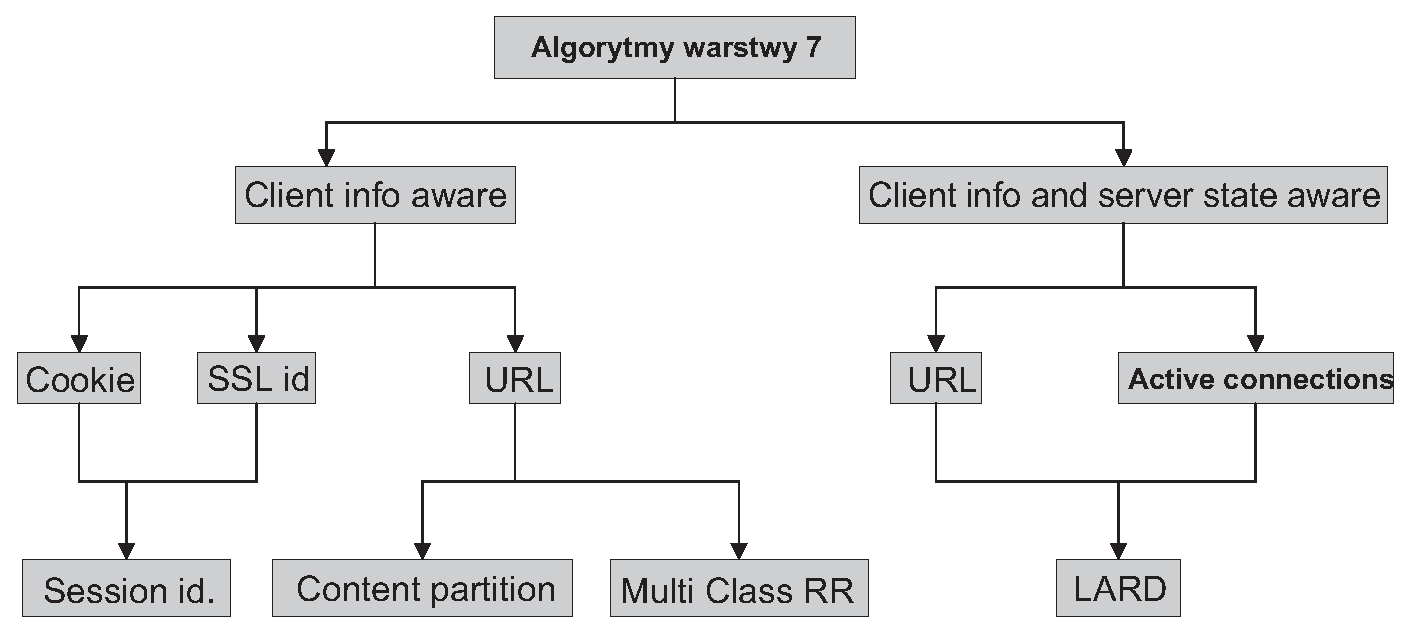
\includegraphics[width=4.9in]{./rysunki/level_7_alg.eps}
\caption{Algorytmy stosowane w prze��cznikach webowych.}
\label{level_7_alg}
\end{figure}

Jak wynika z rysunku \ref{level_7_alg}, istniej� trzy rodzaje algorytm�w opartych na informacjach o kliencie:
\begin{itemize}
\item Session identifiers -- odwo�ania HTTP, maj�ce ten sam identyfikator SSL lub ten sam znacznik cookie przypisywane s� do 
tego samego serwera -- zmniejsza to czas konieczny na ponown� identyfikacj� klienta,
\item Content partition -- podzia� zasob�w serwer�w mo�e nast�pi� ze wzgl�du na:
\begin{itemize}
\item typy plik�w -- dane, pliki graficzne, pliki audio umieszczone s� na specjalizowanych serwerach,
\item wielko�� plik�w -- du�e pliki na szybszych serwerach lub r�wnomierne roz�o�enie plik�w w przypadku serwer�w 
homogenicznych, 
\end{itemize}
\item Multi--class round--robin -- zasoby s� podzielone ze wzgl�du na z�o�ono�� obliczeniow� i czasow�, jaka zostanie 
wygenerowana podczas ich obs�ugi, np. po��czenia szyfrowane wymagaj� mocy obliczeniowej procesora, odwo�ania do bazy danych 
wymagaj� zwi�kszonej obs�ugi dysk�w, czy wreszcie pobieranie du�ych plik�w w znacznym stopniu obci��a sie�.
\end{itemize}

Zasada dzia�ania algorytmu wykorzystuj�cego informacje o kliencie i serwerze jest nast�puj�ca. Pierwsze zapytanie klienta o 
zasoby przekierowywane jest wed�ug algorytmu Least loaded server (metryk� jest ilo�� aktywnych po��cze� z serwerem). Pozosta�e 
zapytania klienta o ten sam zas�b przekierowywane s� do tego samego serwera. Dzi�ki temu zwi�kszona jest skuteczno�� odwo�a� 
do pami�ci podr�cznej (cache) tego serwera. Algorytm ten zwany jest Locality-Aware Request Distribution (LARD).

\subsection{Algorytmy szeregowania wykorzystywane w przypadku przekierowa� na poziomie protoko�u HTTP}

Gdy stosuje si� rozwi�zania oparte na warstwowej strukturze, istnieje mo�liwo�� zarz�dzania zapytaniami z poziomu protoko�u \cite{modele18}. 
Takie rozwi�zanie jest przezroczyste dla u�ytkownik�w. G��wnym celem stosowania tego mechanizmu jest zapobieganie 
przeci��eniom serwer�w webowych. Przekierowywanie odbywa si� poprzez przes�anie klientowi informacji w nag��wku: HTTP OK. 
302 -- Moved temporary to a new location.

Adres nowej lokalizacji mo�e by� podany w postaci nazwy domenowej lub adresu IP. Podanie adresu IP jest bardziej efektywne, 
poniewa� nast�puje bezpo�rednie odwo�anie do nowego serwera (klastra), a nie do serwera DNS.
Przekierowania mo�na realizowa� w zale�no�ci od kilku parametr�w \cite{modele13}. Proces przekierowa� mo�e dotyczy�:
\begin{itemize}
\item wszystkich stron,
\item tylko stron przekraczaj�cych okre�lon� wielko��,
\item tylko stron, kt�rych ilo�� obiekt�w sk�adowych przekracza okre�lon� liczb�,
\end{itemize}

Wyb�r serwera, kt�ry powinien przej�� zapytanie, mo�e odbywa� si� z wykorzystaniem jednej z poni�szych strategii:
\begin{itemize}
\item Round--robin,
\item Least Loaded,
\item Hash function,
\item Client to server proximity.
\end{itemize}

\section{Metody r�wnowa�enia obci��e� -- przyk�ady}

\subsubsection{R�wnowa�enie obci��e� z wykorzystaniem filtra datagram�w}

Inn� implementacj� rozproszonego algorytmu wsp�dzielenia obci��e� jest zastosowanie na ka�dym serwerze 
wchodz�cym w sk�ad klastra tzw. filtra datagram�w. Klaster taki powinien by� po��czony z Internetem poprzez 
pojedynczy router brzegowy. Ka�dy serwer w klastrze posiada skonfigurowane dwa adresy IP: adres ,,prywatny'' i 
jednakowy dla wszystkich serwer�w adres IP klastra. Router po otrzymaniu datagramu opatrzonego adresem IP 
klastra nadaje mu fizyczny (sprz�towy np. adres Ethernet) adres typu broadcast (je�eli do routera przy��czone 
s� tylko serwery nale��ce do klastra) lub multicast (je�eli klaster jest tylko wyr�nion� grup� w�r�d 
wszystkich host�w przy��czonych do serwera). Zastosowanie takiego adresu sprawia, �e karty sieciowe wszystkich 
serwer�w w klastrze akceptuj� datagram. Pomi�dzy sterownikiem karty sieciowej, a oprogramowaniem TCP/IP na 
ka�dym serwerze musi pracowa� specjalny proces, kt�ry zadecyduje, czy pakiet nale�y odrzuci� czy obs�u�y�. 
Proces ten nazywamy filtrem pakiet�w \cite{barylo34}. Decyzja o odrzuceniu lub obs�u�eniu datagramu podejmowana jest na 
podstawie zawarto�ci dw�ch struktur danych: tablicy po��cze� TCP (datagramy nale��ce do jednego po��czenia 
TCP musz� by� obs�ugiwane przez serwer kt�ry nawi�za� dane po��czenie) oraz tablicy zawieraj�cych wielko�� 
obci��enia poszczeg�lnych serwer�w klastra. Tablica ta jest uaktualniana przez same serwery. Ka�dy serwer musi 
wysy�a� okresowo komunikat typu broadcast zawieraj�cy wielko�� jego obci��enia. Je�eli do klastra nadchodzi 
datagram otwieraj�cy nowe po��czenie TCP (nag��wek TCP zawiera flag� SYN) serwer o najni�szym indeksie 
obci��enia w tablicy (indeksem tym jest zwykle liczba otwartych po��cze� TCP) jest zobowi�zany do jego 
przyj�cia. Dla zwi�kszenia wydajno�ci klastra w serwerach stosowa� mo�na dwie karty sieciowe: jedn� ze 
skonfigurowanym adresem IP klastra i drug� z prywatnym adresem serwera.  W takim przypadku pakiety, kt�re nie 
musz� by� filtrowane (np. wymiana danych SNMP) przechodzi� b�d� przez  ,,prywatn�'' kart�. Ten typ r�wnowa�enia 
dotyczy� mo�e ka�dej us�ugi korzystaj�cej z TCP, w szczeg�lno�ci WWW.
Pierwsz� komercyjn� implementacj� tego rozwi�zania by� pakiet oprogramowania Convoy Cluster firmy 
Valence Research przeznaczony dla systemu Microsoft Windows NT. Jako miar� obci��enia serwera przyj�to w nim 
ilo�� otwartych po��cze� TCP, a komunikaty og�aszaj�ce stan obci��enia wysy�ane by�y przez serwery co sekund�. 
Oprogramowanie umo�liwia�o dynamiczn� konfiguracj� klastra przez dodawanie lub usuwanie serwera z klastra bez 
przerywania pracy klastra. Serwery w klastrze musia�y powiela� swoje dane. W pierwszej wersji wymagane by�o 
stosowanie dw�ch kart sieciowych na ka�dym serwerze, a nadchodz�ce datagramy rozg�aszane by�y w trybie broadcast 
(dociera�y do ka�dego hosta w sieci lokalnej klastra, nawet je�li nie by� on serwerem) Wersja 2.0 Convoy 
Cluster wyeliminowa�a te niedogodno�ci i oferowa�a liczne dodatkowe mo�liwo�ci konfiguracyjne np. opcjonalne 
stosowanie pokrewie�stwa z klientem (ang. \emph{client affinity}), co umo�liwia obs�ug� wszystkich datagram�w 
nadchodz�cych od raz zidentyfikowanego (w trakcie nawi�zywania pierwszego po��czenia) klienta przez jeden 
serwer. W roku 1999 firma Microsoft wykupi�a od Valence Research technologi� Convoy Cluster i po 
,,kosmetycznych'' zmianach udost�pni�a j� w pakiecie Microsoft Windows NT 4.0 Enterprise Server pod nazw� 
Microsoft Load Balancing Service.
Najwa�niejsz� zalet� stosowania filtra pakiet�w jest jego du�a wydajno�� w por�wnaniu do 
scentralizowanych urz�dze� rozdzielaj�cych zadania (np. LSNAT). Uzyskiwane jest to dzi�ki temu, �e na �adnym 
etapie obs�ugi zadania nie s� modyfikowane datagramy i nie istnieje pojedynczy punkt podejmowania decyzji o 
obs�udze zadania. Wa�na jest r�wnie� �atwo�� konfiguracji klastra i du�a niezawodno�� (serwer, kt�ry ulega 
awarii przestaje wysy�a� komunikaty o stanie swego obci��enia, nie jest wi�c uwzgl�dniany w tablicach obci��enia 
serwer�w w pozosta�ych w�z�ach klastra i w ten spos�b nie bierze udzia�u w r�wnowa�eniu obci��e�). Koszt jaki 
nale�y ponie��, aby uzyska� te niew�tpliwie po��dane cechy to trudniejsza konfiguracja poszczeg�lnych serwer�w 
(konieczno�� instalacji i konfiguracji filtra pakiet�w) oraz du�y ruch w sieci lokalnej klastra wynikaj�cy z 
aktualizacji tablic obci��enia. Aktualizacje te musz� by� cz�ste, gdy� �atwo mo�na wyobrazi� sobie sytuacj�, w 
kt�rej serwer o najni�szym indeksie obci��enia ulega awarii. W takiej sytuacji pozosta�e serwery a� do 
aktualizacji swoich tablic obci��enia b�d� odrzuca� wszystkie datagramy otwieraj�ce nowe po��czenia, co z 
pewno�ci� nie jest zjawiskiem po��danym.

\subsubsection{R�wnowa�enie obci��e� z wykorzystaniem redirekcji HTTP}

Redirekcja jest  mechanizmem protoko�u HTTP, kt�ry zaprojektowano z my�l� o obs�udze sytuacji w kt�rych 
zas�b (plik) wskazywany przez pewien URL zmienia swoje fizyczne po�o�enie (zostaje przeniesiony na inny serwer) 
i w zwi�zku z tym uzyskuje inny URL. Aby nie zmusza� u�ytkownika do poszukiwania tego zasobu na w�asn� r�k� 
serwer WWW przechowuje tzw. tablice redirekcji. Jest to tablica zawieraj�ca URL, kt�re wcze�niej dotyczy�y 
zasob�w danego serwera, lecz obecnie zasoby te znajduj� si� pod innym URL. Tablica zawiera r�wnie� aktualny URL 
dla ka�dego przeniesionego zasobu. W przypadku zapytania o taki ,,zdezaktualizowany'' URL serwer WWW zwraca 
odpowied� HTTP typu ,,przeniesiono'' i jako dane przekazuje aktualny URL zasobu. Przegl�darka po otrzymaniu takiej 
odpowiedzi musi zestawi� nowe po��czenie z serwerem wskazanym przez otrzymany URL.

Opisany mechanizm w prosty spos�b wykorzysta� mo�na do pewnego rodzaju r�wnowa�enia obci��e� serwer�w 
WWW \cite{barylo22,barylo23}. W klastrze serwer�w wydzieli� mo�na tzw. serwer redirekcji, kt�rego nazwa DNS reprezentowa� 
b�dzie ca�y klaster. Jedynym zadaniem takiego serwera jest utrzymywanie tablicy redirekcji i przekierowanie 
nadchodz�cych zapyta� do odpowiedniego serwera z klastra. W takiej architekturze serwery zwykle nie powielaj� 
swych zasob�w, ka�dy z nich przechowuje cz�� danych udost�pnianych przez klaster, a to kt�ry z nich obs�u�y 
zapytanie determinowane jest przez rodzaj ��danych informacji. Przyk�adowo je�li pod nazw� www.pogoda.com 
dost�pny jest serwis prezentuj�cy prognoz� pogody dla ka�dego kontynentu to zasoby serwisu podzieli� mo�na 
pomi�dzy siedem serwer�w (po jednym dla ka�dego kontynentu) a pod adresem IP stanowi�cym odwzorowanie nazwy 
serwisu nale�y umie�ci� serwer redirekcji. W odpowiedzi na zapytanie o dowolny URL zaczynaj�cy si� np. od ci�gu 
www.pogoda.com/Azja/ serwer redirekcji dokonywa�by przekierowania do serwera przechowuj�cego dokumenty o 
pogodzie w Azji (np. wwwazja.pogoda.com) \cite{barylo22}. Poni�szy rysunek przedstawia schemat nawi�zywania 
po��czenia w przypadku stosowania redirekcji HTTP:
\begin{figure}[h]
\centering
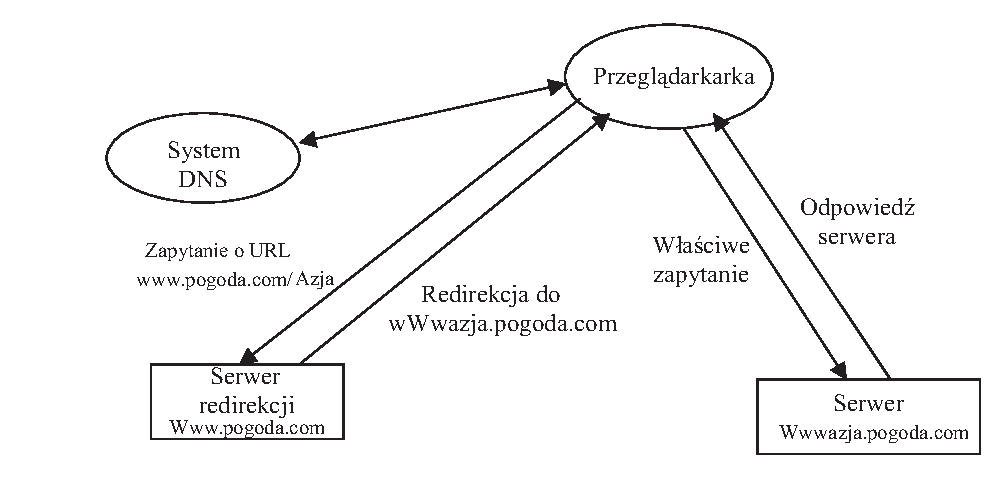
\includegraphics[width=4.9in]{./rysunki/redirekcja.eps}
\caption{Schemat redirekcji HTTP.}
\label{redirekcja}
\end{figure}

Stosowanie redirekcji ma zasadniczo dwie zalety. Po pierwsze utrzymanie statycznej tablicy redirekcji jest 
bardzo proste i tanie w implementacji, nie wymaga stosowania specjalnego sprz�tu ani oprogramowania. Po drugie, 
poniewa� u�ywane s� adresy URL, klaster stanowi�cy logiczn� ca�o�� mo�e by� rozproszony geograficznie tzn. 
serwer prezentuj�cy dane o pogodzie w Azji mo�e rzeczywi�cie znajdowa� si� na terenie tego kontynentu, co mo�e 
by� dobrym pomys�em przy za�o�eniu, �e o pogod� w Azji pyta� b�d� g��wnie Azjaci.
Redirekcja ma jednak wiele wad \cite{barylo30}. Przede wszystkim ograniczona jest do protoko�u HTTP, a jak wiadomo 
wiele ��cz hipertekstowych dokonuje prze��czenia do np. serwer�w FTP, kt�re cz�sto pracuj� na fizycznie tych 
samych komputerach, co serwery WWW. Druga wada jest wyra�nie widoczna na Rys. \ref{redirekcja}. Aby rozpocz�� pobieranie 
��danego dokumentu przegl�darka musi dokona� dw�ch po��cze�, najpierw z serwerem redirekcji, a nast�pnie z 
w�a�ciwym serwerem. Wprowadza to znaczne op�nienie i powoduje dodatkowe obci��enie sieci, kt�ra jest cz�sto 
w�skim gard�em wydajno�ci WWW. 

Prezentowane powy�ej podej�cie jest z gruntu statyczne i zak�ada wiedz� o tym, kt�re dane b�d� 
poszukiwane najcz�ciej, co umo�liwia aprioryczne przydzielenie najsilniejszego serwera w klastrze do obs�ugi 
najpopularniejszej cz�ci serwisu WWW. Poniewa� tablica redirekcji nie zawiera �adnych danych o obci��eniu 
poszczeg�lnych serwer�w trudno jest  dynamicznie uwzgl�dnia� takie dane podczas wyboru serwera. W literaturze 
proponowano architektury pi�trowe. Przyk�adowo dane dotycz�ce pogody w Azji mog�yby by� powielane pomi�dzy 
kilka serwer�w, kt�re raportowa�yby stopie� swego obci��enia, a na podstawie tych danych serwer redirekcji 
m�g�by dynamicznie aktualizowa� tablice redirekcji. Zbyt cz�sta aktualizacja tej tablicy czyni j� jednak 
bezu�yteczn� (tablica jest niedost�pna w trakcie aktualizacji), a zbyt rzadka powoduje nier�wnomierno�� 
obci��enia. Innym rozwi�zaniem jest zachowanie podzia�u na serwery tematyczne z mo�liwo�ci� dynamicznego 
przeniesienia cz�ci zawarto�ci z serwera mocno obci��onego na serwer posiadaj�cy rezerw� wydajno�ci. 
Aktualizacje tablicy redirekcji by�yby wtedy rzadsze, lecz procedura taka wymaga�aby kosztownego �ledzenia, 
kt�re pliki pobierane s� najcz�ciej (tylko przeniesienie takich plik�w znacz�co mo�e zmniejszy� obci��enie 
serwera), dodatkowo dane by�yby niedost�pne przez czas przenoszenia. Obydwie metody dynamicznego wykorzystania 
tablicy redirekcji mog� by� omini�te przez u�ytkownika, je�li po po��czeniu z serwerem docelowym umie�ci on 
zak�adk� (ang. \emph{bookmark}) na pobieranych stronach WWW. 
Statyczna redirekcja HTTP jest skuteczna tylko w przypadku serwis�w charakteryzuj�cych si� �atwym do 
przewidzenia wzorcem dost�pu do dokument�w.

\subsubsection{R�wnowa�enie obci��e� z wykorzystaniem NAT}

Mechanizm translacji adres�w sieciowych NAT (ang. \emph{Network Address Translation}) zosta� zaprojektowany z 
my�l� o mo�liwo�ci w��czenia prywatnych sieci lokalnych do Internetu z wykorzystaniem jednego, globalnie 
unikalnego adresu IP dla ca�ej sieci. W standardowej konfiguracji urz�dzeniem realizuj�cym NAT jest router 
brzegowy o adresie IP reprezentuj�cym ca�� sie�, kt�ry stanowi jedyne po��czenie pomi�dzy sieci� prywatn� a 
rozleg��. Hosty w sieci prywatnej nie musz� posiada� globalnie unikalnych adres�w IP, gdy� podczas nawi�zywania 
po��czenia z komputerem spoza sieci prywatnej urz�dzenie NAT zamienia adres nadawcy datagramu IP (pochodz�cy z 
sieci prywatnej) na sw�j w�asny, dokonuje przeliczenia odpowiednich sum kontrolnych i aby poprawnie kierowa� 
datagramami nale��cymi do jednego po��czenia TCP zapami�tuje w wewn�trznych tablicach parametry po��czenia 
(adresy i porty �r�d�owe i docelowe). Celem wprowadzenia mechanizmu NAT by�o zapewnienie pewnego stopnia 
bezpiecze�stwa sieciom prywatnym, gdy� je�li wewn�trz takiej sieci komputery nie posiadaj� globalnie unikalnych 
adres�w IP, to nie istnieje mo�liwo��  nawi�zania po��czenia z takim komputerem spoza sieci prywatnej. 
Istnieje wiele rozwi�za� komercyjnych realizuj�cych r�wnowa�enie (wsp�dzielenie)  obci��e� serwer�w 
WWW poprzez mechanizm NAT. Idea polega na kierowaniu zapyta� nadchodz�cych do klastra serwer�w poprzez 
specjalizowane urz�dzenie NAT, okre�lane czasem jako LSNAT (ang. \emph{Load Sharing NAT}), kt�re kierowa�oby zapytanie 
do konkretnego serwera \cite{barylo7}. Algorytm wed�ug kt�rego zapytanie by�yby kierowane do serwer�w mo�e uwzgl�dnia� 
r�nice w ich wydajno�ci jak i stopie� ich obci��enia, istnieje r�wnie� mo�liwo�� uwzgl�dnienia w nim numeru 
portu TCP, co sprawia, �e LSNAT stosowa� mo�na do r�wnowa�enia obci��e� wszystkich us�ug TCP. Obci��enie 
serwer�w okre�lane jest zazwyczaj na podstawie tablicy otwartych po��cze� utrzymywanej przez LSNAT dla ka�dego 
serwera. Aby dane te by�y aktualne konieczna jest analiza nag��wk�w TCP w celu wykrywania datagram�w 
zamykaj�cych po��czenie. Serwery w klastrze powinny powiela� swoje dane, gdy� wykorzystanie rozproszonego 
systemu plik�w powoduje zbyt du�e obci��enie sieci lokalnej klastra. Poni�ej schematycznie przedstawiono dwie 
typowe konfiguracje urz�dzenia NAT jako modu�u realizuj�cego  r�wnowa�enie obci��e�. Na ka�dym rysunku klaster 
serwer�w reprezentowany jest przez adres IP 172.87.0.100.

W takiej konfiguracji w datagramach przychodz�cych do klastra nast�puje zmiana adresu docelowego z adresu 
urz�dzenia LSNAT na adres wybranego serwera oraz zmiana adresu nadawcy na adres urz�dzenia LSNAT. W datagramach 
wysy�anych w przeciwnym kierunku adres nadawcy zmienia si� z adresu serwera na adres LSNAT a adres docelowy z 
adresu LSNAT na adres rzeczywistego odbiorcy datagramu. Takie post�powanie powoduje, �e wszystkie datagramy 
kierowane do klastra i z powrotem musz� przej�� przez urz�dzenie LSNAT, co umo�liwia skonfigurowanie klastra 
rozproszonego geograficznie. Dzieje si� tak kosztem utrzymywania w LSNAT bardziej rozbudowanej (w stosunku do 
poprzedniej konfiguracji) tablicy po��cze�, kt�ra umo�liwia�aby identyfikacj� ka�dego po��czenia. Identyfikacji 
tej dokonuje si� wykorzystuj�c numery port�w TCP (wraz z translacj� adres�w datagramu dokonuje si� zmiany 
numeru portu �r�d�owego na unikaln� dla danego serwera warto�� powy�ej 5000, identyfikacji odpowiedzi adresata
dokonuje si� na podstawie adresu serwera, kt�ry j� wys�a� i numeru portu docelowego). Powy�sza konfiguracja 
pracowa� mo�e r�wnie� z adresami prywatnymi, uniemo�liwia to jednak u�ycie serwer�w odleg�ych geograficznie.
Poni�ej przedstawiono kr�tki opis dw�ch popularnych rozwi�za� komercyjnych wykorzystuj�cych mechanizm 
NAT do r�wnowa�enia obci��e� serwer�w WWW.

Rozwi�zania korzystaj�ce z mechanizmu NAT do r�wnowa�enia obci��e� s� znacznym post�pem w stosunku do metod 
opisanych wcze�niej w tej pacy. Umo�liwiaj� skuteczne uwzgl�dnienie stopnia obci��enia poszczeg�lnych serwer�w 
w klastrze jak i ich indywidualnych w�a�ciwo�ci. LSNAT umo�liwia rozr�nianie po��cze� na podstawie numer�w 
port�w TCP jak i r�wnowa�enie obci��e� pomi�dzy serwery odleg�e geograficznie. Metoda ta nie jest jednak 
pozbawiona wad. W oczywisty spos�b urz�dzenie LSNAT staje si� w�skim gard�em wydajno�ci klastra, gdy� ca�y 
ruch pomi�dzy klasterem, a Internetem musi przez nie przechodzi�. Je�li wzi�� pod uwag�, �e w przypadku WWW 
obj�to�� odpowiedzi serwera jest co najmniej dziesi�ciokrotnie wi�ksza ni� zapytanie, jasnym staje si�, �e w 
obliczu ci�g�ego wzrostu liczby u�ytkownik�w, najwydajniejsze nawet urz�dzenie LSNAT mo�e w ko�cu ograniczy� 
wydajno�� klastra. Nale�y r�wnie� zauwa�y�, �e zmiana adresu IP w nag��wku datagramu poci�ga za sob� 
konieczno�� wyliczenia nowej sumy kontrolnej dla ca�ego datagramu. Jest to operacja czasoch�onna przez co 
wprowadza op�nienie w transmisji danych jak i konieczno�� kolejkowania pakiet�w w samym urz�dzeniu (trudno 
oczekiwa�, �e nawet urz�dzenie przetwarzaj�ce klika pakiet�w r�wnolegle poradzi sobie bez op�nie� z ca�ym 
przechodz�cym przez nie ruchem). Ta w�a�ciwo�� LSNAT znacznie ogranicza jego skalowalno��, gdy� dodawanie 
nowych serwer�w do klastra w prosty spos�b zwi�ksza kolejk� pakiet�w w urz�dzeniu, a� do momentu, w kt�rym 
przekroczone zostan� jego mo�liwo�ci lub cierpliwo�� u�ytkownik�w. 

\subsubsection{R�wnowa�enie obci��e� poprzez ,,p�--po��czeniowe'' marszrutowanie TCP}

Rozpatruj�c przedstawione kolejno w tej pracy metody r�wnowa�enia obci��e� mo�na zauwa�y� pewn� 
prawid�owo��. Ot� im dana metoda jest bardziej skuteczna i zaawansowana koncepcyjnie, tym w ni�szej warstwie 
sieciowej operuje. Redirekcja HTTP i RR--DNS dzia�a�y powy�ej warstwy transportowej, w og�le nie ingeruj�c w 
zawarto�� datagram�w IP. Rozwi�zania oparte o LSNAT i DPR pracowa�y w warstwie sieciowej i aby skutecznie 
rozdziela� zadania pomi�dzy serwery musia�y dokonywa� modyfikacji (adres�w i sum kontrolnych) w nag��wkach  
datagram�w IP. Metoda opisana w tym punkcie operuje w warstwie fizycznej  i do rozdzia�u zada� nie musi 
zmienia� zawarto�ci datagram�w IP.

,,P�--po��czeniowe'' marszrutowanie TCP (ang. \emph{half--connection TCP routing}) jest opatentowan� przez 
firm� IBM technologi�, kt�ra leg�a u podstaw zasady dzia�ania pakietu oprogramowania Network Dispatcher \cite{barylo35,barylo36}. 
W swej podstawowej konfiguracji pakiet ten umo�liwia zestawienie klastra z�o�onego z po��czonych 
sieci� lokaln� serwer�w korzystaj�cych TCP lub UDP (w szczeg�lno�ci serwer�w WWW) i udost�pnienie go pod 
jednym adresem IP. W klastrze tym serwery maj� unikalne globalnie lub lokalnie adresy IP i  musz� powiela� 
swoje dane. W obszarze tej samej sieci lokalnej, w kt�rej dzia�a klaster, musi by� wyznaczony komputer, na 
kt�rym pracowa� b�dzie oprogramowanie Network Dispatcher. Komputer ten musi posiada� dwa adresy IP, jeden z 
nich, tzw. adres NFA (ang. \emph{Non--Forwarding Address}) jest ,,osobistym'' adresem komputera, pod kt�rym mo�na 
skontaktowa� si� z pracuj�cym na tym komputerze oprogramowaniem (np. z agentem SNMP). Drugi adres, to adres 
reprezentuj�cy klaster serwer�w, wszystkie datagramy IP opatrzone tym adresem b�d� przetwarzane przez program 
Network Dispatcher i na podstawie algorytmu wsp�dzielenia obci��e� przekazywane do jednego z serwer�w w 
klastrze. Dispatcher zmienia jedynie docelowy adres fizyczny (sprz�towy) datagramu, zawarty w nag��wku 
sprz�towym, dodawanym przed nag��wek IP (np. w nag��wku Ethernet). Dzi�ki temu datagramy wysy�ane przez serwer 
w odpowiedzi mog� by� kierowane bezpo�rednio do klienta, bez konieczno�ci ponownego przej�cia przez 
oprogramowanie Network Dispatcher (w celu np. przywr�cenia oryginalnych adres�w IP). St�d pochodzi nazwa tej 
metody -- ,,p�--po��czeniowe'' marszrutowanie TCP. Serwer wysy�aj�c odpowied� dokonuje standardowej zamiany adres�w 
IP nadawcy i odbiorcy pobieraj�c obydwa te adresy z nag��wka otrzymanego datagramu. Jak pami�tamy adresem 
docelowym jest w tym datagramie adres klastra (komputera, na kt�rym pracuje Dispatcher), wi�c adres ten stanie 
si� adresem nadawcy odpowiedzi, co sprawi, �e kolejne datagramy dotycz�ce danego po��czenia skierowane zostan� 
na adres Network Dispatcher--a \cite{barylo36}.

Adres IP ka�dego serwera w klastrze jest r�ny od adresu klastra. Fakt, �e pomimo to oprogramowanie 
TCP/IP w serwerze akceptuje pakiety opatrzone adresem klastra jest mo�liwy dzi�ki dodaniu aliasu do adresu 
interfejsu p�tli zwrotnej (ang. \emph{loopback interface}) w ka�dym serwerze. Do standardowego adresu 127.0.0.1 
dodawany jest jako alias adres klastra (w przypadku przedstawionym na rysunku 139.37.38.39). Mo�liwo�� 
nadawania wielu adres�w interfejsowi p�tli zwrotnej jest jedynym wymaganiem Dipatcher-a w stosunku do serwer�w.
Poniewa� Network Dispatcher rozr�nia porty TCP i UDP mo�liwe jest r�wnowa�enie obci��e� powodowanych 
przez dowolny protok� korzystaj�cy z TCP lub UDP m.in. HTTP (WWW), FTP, SSL, SMTP, POP3 czy Telnet. Poniewa� 
wszystkie serwery powielaj� swoje dane, mo�liwa jest sytuacja w kt�rej np. plik HTML opisuj�cy stron� WWW 
pobierany jest z serwera A, a pliki graficzne sk�adaj�ce si� na stron� pobierane s� z serwera B.
W celu zarz�dzania po��czeniami Network Dispatcher przechowuje dwie struktury danych- tablic� po��cze� 
aktywnych (otwartych) i tablic� nowo przydzielonych po��cze�. Tablica otwartych po��cze� s�u�y do poprawnego 
kierowania datagram�w dotycz�cych nawi�zanego po��czenia TCP (po��czenie TCP nie mo�e by� przez Dipatcher 
przekazane pomi�dzy serwerami). Zawiera ono adres IP nadawcy i numer �r�d�owego portu TCP oraz adres IP serwera, 
kt�ry obs�uguje po��czenie i numer portu docelowego TCP oraz pole stanu po��czenia. Pozycje z tej tablicy s� 
usuwane po wykryciu w nag��wku TCP flagi FIN lub RST. Ilo�� po��cze� otwartych na danym serwerze jest r�wnie� 
uwzgl�dniana podczas obliczenia wagi serwera. Tablica nowo przydzielonych po��cze� s�u�y do zapami�tania jak 
wiele po��cze� zosta�o przydzielonych do danego serwera od ostatniego od�wie�enia wag serwer�w i jako miara 
pr�dko�ci zmian obci��enia serwera wykorzystywana jest do obliczenia jego wagi.

Je�eli na adres Dispatcher--a przychodzi datagram nie nale��cy do �adnego z po��cze� zapisanych w 
tablicy aktywnych po��cze�, oznacza to, �e jest to nowe po��czenie i nale�y przydzieli� serwer do jego obs�ugi. 
Dispatcher utrzymuje cykliczn� list� serwer�w zawieraj�c� ich wagi. Waga serwera oddaje stopie� jego obci��enia 
i jest obliczana przez Dispatcher okresowo dla klastra (dla wszystkich serwer�w jednocze�nie). Dispatcher 
pami�ta numer i wag� serwera do kt�rego przydzielono ostatnie po��czenie TCP i rozpoczynaj�c przeszukiwanie 
listy od tego miejsca poszukuje serwera o wadze wi�kszej lub r�wnej zapami�tanej wadze (im wi�ksza waga, tym 
mniej obci��ony serwer). Do znalezionego w ten spos�b serwera przydzielane jest nowe po��czenie, co znajduje 
odwzorowanie w tablicy aktywnych po��cze�. 

Waga dla ka�dego serwera obliczana jest na podstawie ilo�ci otwartych po��cze� TCP, ilo�ci nowo 
przydzielonych po��cze�, stopnia obci��enia procesora w serwerze (miara ta uwzgl�dnia r�wnie� obci��enie 
wynikaj�ce z zada� uruchamianych lokalnie i pochodzi od modu�u ISS (ang. \emph{Interactive Session Support}) pakietu 
Network Dispatcher, ISS uwzgl�dnia r�wnie� indywidualne w�a�ciwo�ci serwera) oraz na podstawie danych 
pochodz�cych z tzw. Advisor--�w. Advisor jest programem symuluj�cym klienta danego protoko�u i bada jak szybko 
serwer jest w stanie zareagowa� na typowe dla danego protoko�u ��danie. Np. Advisor HTTP wysy�a do serwera 
��danie HTTP GET / (prze�lij domy�lny dokument g��wnego katalogu w serwisie) i jako wynik zwraca czas, po kt�rym 
otrzyma� pierwszy bajt odpowiedzi. Proporcje z jakimi poszczeg�lne elementy wchodz� w sk�ad wagi, jak i 
cz�stotliwo�� od�wie�ania wag ustalane s� przez administratora klastra.
Network Dispatcher posiada wiele cech wyr�niaj�cych go spo�r�d przedstawionych wcze�niej rozwi�za�. 
Jest oczywi�cie wolny od niekorzystnych cech RR--DNS i nie modyfikuje datagram�w IP, a analiza, kt�r� na nich 
prowadzi (zapami�tanie adres�w i port�w, wykrywanie flag), nie jest czasoch�onna. Dodatkowo ruch przechodz�cy 
przez Dispatcher--a stanowi� tylko datagramy nadchodz�ce do klastra (typowo mniejsze od odpowiedzi), dzi�ki 
czemu nie jest �atwo (w przeciwie�stwie do urz�dze� LSNAT) tak obci��y� Dispatcher--a by sta� si� ,,w�skim 
gard�em'' wydajno�ci klastra. W przeciwie�stwie do rozwi�zania z zastosowaniem DPR, Dispatcher nie wymaga 
specjalistycznego oprogramowania pracuj�cego na serwerze, wi�c nie obci��a go np. zadaniem przetwarzania 
datagram�w IP.

Pierwszy prototyp Network Dispatcher--a obs�ugiwa� Internetowy serwis IO w Atlancie w 1996. Kolejne, 
ju� komercyjne wersje obs�ugiwa�y takie wydarzenia jak turniej US Open i IO w Nagano w 1998 oraz mecze szachowe 
Deep Blue vs. Garri Kasparow. Szczytowe obci��enie klastra w przypadku IO w Nagano osi�gn�o 110 414 zapyta� na
 minut�, a mimo to r�wnowa�enie obci��e� przy u�yciu Network Dispatcher--a zapewni�o wszystkim u�ytkownikom dobry 
czas odpowiedzi i zadowalaj�cy transfer.

\subsubsection{R�wowa�enie obci��e� poprzez bezpo�rednie routowanie -- \emph{Direct Routing}}

Architektura ta jest podobna do wykorzystywanej w produkcie firmy IBM -- oprogramowaniu SecureWay Network Dispatcher. 

Adres wirtualny serwera jest wsp�dzielony poprzez poszczeg�lne nody i load balancer. Interfejs sieciowy dystrybutora jest 
skonfigurowany tak�e do wirtualnego adresu, kt�ry jest wykorzystywany do przyjmowania pakiet�w przychodz�cych oraz do 
bezpo�redniego routowania pakiet�w do wybranych serwer�w. Wszystkie rzeczywiste serwery maj� swoje non--arp aliasy interfejsu 
sieciowego skonfigurowane z adresem wirtualnym lub bezpo�rednio przekierowuj� pakiety przeznaczone na adres wirtualny do 
lokalnych gniazd, w ten spos�b, �e rzeczywiste serwery mog� przenosi� pakiety tylko lokalnie. Zar�wno load balancer jak i 
rzeczywiste serwery musz� mie� interfejsy sieciowe fizycznie skojarzone z HUB--em lub switchem. Wygl�da to w ten spos�b, �e
dystrybutor po prostu zmienia adres MAC na adres rzeczywistego serwera i retransmituje do niego pakiet. 

\section{Przyk�ady produkt�w stosowanych do r�wnowa�enia obci��enia wielokomputerowych serwer�w WWW}

\subsection{LinuxVirtualServer}

Linux Virtual Server jest wysoce skalowalnym i dost�pnym serwerem zbudowanym na klastrze rzeczywistych serwer�w wraz 
z mo�liwo�ci� realizacji r�wnowa�enia obci����. System ten oparty jest na systemie Linux. Architektura tego rozwi�zania
jest (jak i pozosta�e) przezroczysta dla klienta i odbywa si� na poziomie protoko�u IP (warstwa czwarta). 

Rzeczywiste serwery mog� by� po��czone w obr�bie sieci lokalnej lub geograficznie rozproszone w sieci WAN. Fron-endem tych
rzeczywistych serwer�w jest dystrybutor (load balancer), kt�ry marszrutuje ��dania do r�nych serwer�w oraz powoduje, �e
r�wnoleg�e us�ugi dzia�aj�ce w obr�bie klastra wydaj� si� by� jedn� wirtualn� us�ug� dla ca�ego klastra na jednym adresie IP.
Skalowalno�� w tym systemie oznacza, �e w przezroczysty spos�b mo�na dodawa� i usuwa� poszczeg�lne nody do klastra. Wysoka 
dost�pno�� jest realizowana poprzez detekcj� uszkodzonych nod�w lub niesprawnych demon�w oraz r�wnoczesn� rekonfiguracj�
systemu.

Virtual Server mo�na implementowa� na trzy sposoby:
\begin{description}
\item[Virtual Server poprzez NAT] -- zalet� tego rozwi�zania jest fakt, �e rzeczywiste serwery mog� pracowa� na dowolnym
systemie operacyjnym, kt�ry w�ada protoko�em TCP/IP. Rzeczywiste serwery maj� prywatny adresy IP i tylko one s� potrzebne
dystrybutorowi do pracy. Wad� tego rozwi�zania jest raczej niewielka skalowalno��, poniewa� w tym wypadku \emph{load balancer}
mo�e stanowi� w�skie gard�o ca�ego systemu gdy liczba pod��czonych serwer�w b�dzie wynosi� oko�o 20 lub wi�cej. Jest to
spowodowane tym, �e zar�wno ruch przychodz�cy (niewielki) jak i wychodz�cy (o wiele wi�kszy) s� przepisywane przez dystrybutora.
Mo�na to omin�c poprzez korzystanie z pozosta�ych rozwi�za� Virtual Servera lub poprzez rozwi�zanie hybrydowe z DNS i kilkoma
osobnymi Virtual Serverami;
\item[Virtual Server poprzez Tunelowanie IP] -- w tym wypadku load balancer tylko przekazuje
ruch wchodz�cy do poszczeg�lnych rzeczywistych serwer�w, za� one odpowiadaj� bezpo�rednio do u�ytkownik�w. W tym rozwi�zaniu 
jak wida� serwer virtualny mo�e si� sk�ada� i z ponad 100 serwer�w i nadal dystrybutor nie b�dzie stanowi� w�skiego gard�a.
Maksymalna wydajno�� Virtual Servera w tym przypadku mo�e si�ga� powy�ej 1Gbps -- w przypadku gdy dystrybutor dysponowa�
b�dzie 100Mbps kart� sieciow�. Rozwi�zanie oparte na tunelowaniu IP mo�e by� u�ywane do serwer�w wirtualnych w bardzo 
wysokich wydajno�ciach, szczeg�lnie dobrych do tworzenia virtualnych proxy serwer�w. Wad� tego rozwi�zania jest to, �e ka�dy
serwer musi umie� dokonywa� enkapsulacji IP (tunelowanie IP) wewn�trz IP; 
\item[Virtual Server poprzez bezpo�rednie routowanie]\footnote{ang. \emph{Direct Routing}} -- opisany powy�ej. Wad� tego 
rozwi�zanie jest brak mo�liwo�ci rozbudowy wirtualnego serwera powy�ej sieci lokalnej, jednak�e w por�wnaniu z poprzedni�
architektur� rzeczywiste serwery nie potrzebuj� pos�ugiwa� si� enkapsulacj� IP.
\end{description}

W po��czeniu z ka�d� implementacj� Virtual Server korzysta z nast�puj�cych algorytm�w dystrubuuj�cych pakiety:
\begin{itemize}
\item marszrutowanie algorytmem Round--Robin;
\item marszrutowanie algorytmem Weighted Round--Robin (statyczne wagi, bez wykorzystywania informacji o stanie system�w);
\item marszrutowanie typu Least Connection (dynamiczny algorytm -- opisany w tekscie);
\item marszrutowanie typu Weighted Least Connection (jak wy�ej + statycznie nadawane wagi poszczeg�lnym serwerom);
\item marszrutowanie Locality--Based Least Connection;
\item marszrutowanie Locality--Based Least Connection witch Replcation;
\item marszrutowanie typu Destination Hashing;
\item marszrutowanie typu Source Hashing.
\end{itemize}

Zalet� Virtual Servera jest jego dzia�anie w obr�bie j�dra co oznacza wysok� wydajno�� i stabilno��. Kolejn� zalet� jest 
dost�pno�� kodu �r�d�owego (oprogramowanie typu OpenSource) co oznacza mo�liwo�� modyfikacji kodu w zale�no�ci od potrzeb.

\subsection{Cisco LocalDirector}

LocalDirector jest nazw� rodziny urz�dze� produkowanych przez firm� Cisco. Urz�dzenia te s�u�� do 
r�wnowa�enia obci��e� dowolnych serwer�w wykorzystuj�cych TCP (np. serwery WWW, FTP, SSL) \cite{barylo30,barylo31}. 
LocalDirector instalowany jest w konfiguracji przedstawionej na Rys. \ref{LocalDirector} z wykorzystaniem adres�w prywatnych, 
\begin{figure}[h]
\centering
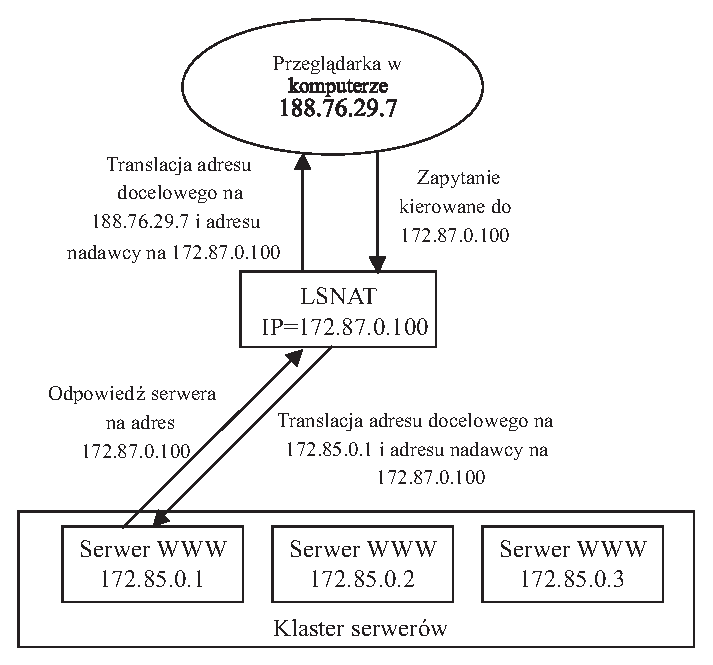
\includegraphics[width=4in]{./rysunki/LocalDirector.eps}
\caption{LSNAT symetrycznie zmieniaj�cy adres IP.}
\label{LocalDirector}
\end{figure}

musi wi�c by� instalowany jako jedyne po��czenie pomi�dzy klasterem a bramk� (ang. \emph{gateway}) do sieci rozleg�ej. 
LocalDirector wymaga powielania zawarto�ci pomi�dzy serwerami w klastrze. Serwery mog� by� po��czone z 
LocalDirector-em poprzez sie� Ethernet, FastEthernet lub FDDI. Wyb�r serwera dokonywany jest sekwencyjnie na 
podstawie wag uwzgl�dniaj�cych indywidualne w�a�ciwo�ci serwera i jego obci��enie w postaci liczby otwartych 
po��cze� TCP. LocalDirector sprawdza czy serwer si� nie za�ama� poprzez okresowe nawi�zywanie z nim po��czenia 
kontrolnego (Ping, HTTP GET /). Producent zapewnia, �e LocalDirector, w zale�no�ci od modelu, jest w stanie 
obs�u�y� od 7000 do 25000 po��cze� na sekund� przy przepustowo�ci od 80 Mbit/sek. do 400 Mbit/sek. Istnieje 
mo�liwo�� pi�trowej konfiguracji LocalDirector-a. Kilka rozproszonych geograficznie klaster�w, z kt�rych ka�dy 
obs�ugiwany jest przez jedno urz�dzenie LocalDirector, mo�na zaprezentowa� jako jeden klaster z u�yciem tzw. 
GlobalDirectora. GlobalDirector to w rzeczywisto�ci serwer DNS rozdzielaj�cy zapytania pomi�dzy klastery na 
zasadzie podobnej do RR--DNS. 

\subsection{F5 Labs BigIP}

BigIP firmy F5 Labs jest tzw. rozwi�zaniem ,,pod klucz'' (ang. \emph{turn--key solution}). Oznacza to, �e dostarczany 
jest tak jak urz�dzenie sprz�towe (np. LocalDirector), cho� w rzeczywisto�ci jest to komputer pracuj�cy pod 
kontrol� specjalizowanego oprogramowania i systemu operacyjnego firmy F5 Labs. BigIP umo�liwia r�wnowa�enie 
obci��e� ka�dego serwera korzystaj�cego z protoko�u TCP lub UDP \cite{barylo32,barylo33}. Urz�dzenie mo�e by� pod��czone w 
konfiguracji przedstawionej na Rys. \ref{LocalDirector} lub Rys. \ref{LocalDirector1} w obydwu jednak przypadkach, aby uniemo�liwi� omini�cie 
\begin{figure}[h]
\centering
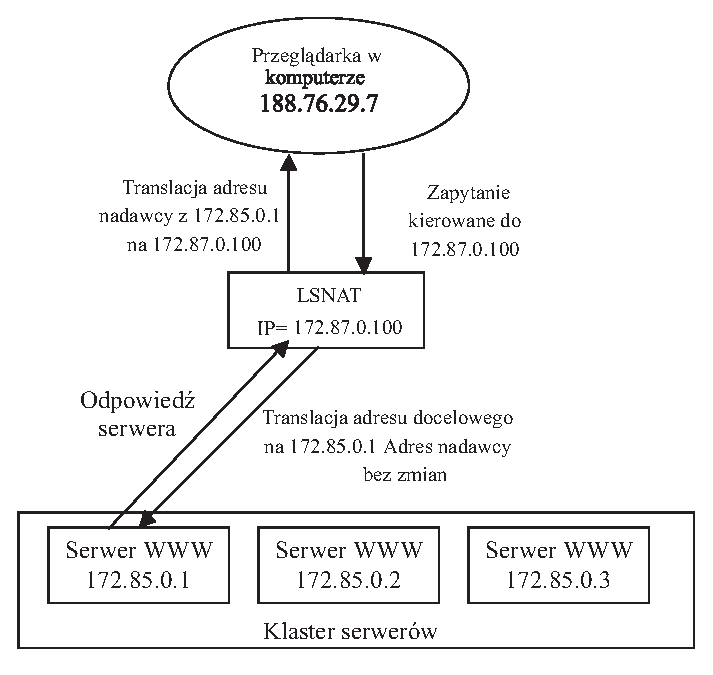
\includegraphics[width=4in]{./rysunki/LocalDirector1.eps}
\caption{LSNAT zmieniaj�cy jeden z adres�w IP}
\label{LocalDirector1}
\end{figure}

mechanizmu r�wnowa�enia obci��e�, BigIP powinien znajdowa� si� pomi�dzy klasterem serwer�w, a bramk� do 
Intetrnet-u. BigIP mo�na po��czy� z klasterem poprzez sie� Ethernet, FastEthernet, FDDI lub opcjonalnie 
GigaBitEthernet. Urz�dzenie oferuje do wyboru siedem algorytm�w rozdzia�u zada�. Trzy z nich to algorytmy 
statyczne, s� to: algorytm cykliczny (ang. \emph{Round--robin}); algorytm proporcjonalny przydzielaj�cy zadania wed�ug 
ustalonych na sta�e wag i algorytm priorytetowy, kt�ry umo�liwia wydzielenie w klastrze grup serwer�w o 
okre�lonym priorytecie i rozdzia� zada� do grup, w ka�dej z grup serwer do obs�ugi konkretnego zadania 
wskazywany jest cyklicznie. Pozosta�e algorytmy s� dynamiczne i uwzgl�dniaj� obci��enie poszczeg�lnych 
serwer�w. S� to algorytm LC (ang. \emph{Least Connections}) przydzielaj�cy zadania do serwera utrzymuj�cego najmniej 
otwartych po��cze�, algorytm wyznaczaj�cy ten serwer, kt�ry najszybciej odpowie na zapytanie kontrolne (np. 
HTTP GET /), tzw. algorytm obserwacyjny b�d�cy kombinacj� powy�szych i algorytm predyktywny, kt�ry przydziela 
zadania (po��czenia) do serwera, kt�rego obci��enie (mierzone jako kombinacja ilo�ci otwartych po��cze� i czasu 
odpowiedzi na zapytanie kontrolne) zmniejsza�o si� najszybciej w ci�gu np. ostatnich 5 sekund.
Konkretne modele BigIP wyposa�one s� w procesory Intel Pentium II 450 do 600 MHz pami�� RAM 128 MB do 
1GB i dysk twardy 4 GB do 8.4 GB. Producent gwarantuje przepustowo�� od 170 Mbit/sek. do 350 Mbit/sek. i 
obs�ug� do 20000 zapyta� na sekund�.
	
\subsection{IBM SecureWay Network Dispatcher}

W zwi�zku z tym, �e pakiet ten jest jednym z g��wnych element�w tej pracy, jego dok�adny opis i konfiguracja znajduje si� 
w nast�pnym rozdziale (Rozdz. \ref{r05}).


\chapter{System do zarz�dzania wielokomputerowym serwerem WWW}
\label{r05}

\section{Wst�p}
W tym rozdziale zostanie przedstawiony opis konfiguracji stanowiska u�ytego do bada� nad charakterystykami 
r�nych konfiguracji i algorytm�w klastra serwer�w WWW zestawionego w �rodowisku systemu AIX i Windows NT z 
wykorzystaniem pakietu IBM WebSphere Performance Pack. Opisana zostanie konfiguracja sieci komputerowej, w kt�rej zosta�y 
przeprowadzone badania oraz charakterystyka poszczeg�lnych test�w.

\section{Charakterystyka u�ytego oprogramowania}

\subsection{IBM WebSphere Performance Pack}

IBM WebSphere Performance Pack jest oprogramowaniem infrastrukturalnym WWW wi���cym ze sob� skalowalno��, niezawodno�� i 
wydajno��, kt�re to cechy s� niezb�dne dla aplikacji e-biznesu zar�wno w �rodowiskach lokalnych jak i rozproszonych. Jego 
funkcje ��cz� ze sob� znakomity caching, zarz�dzanie plikami i r�wnowa�enie obci��enia, kt�re razem kompensuj� wrodzone 
s�abo�ci Internetu by wspiera� krytyczne aplikacje biznesowe.

IBM WebSphere Performance Pack sk�ada si� z trzech g��wnych element�w, kt�re to pozwalaj� zredukowa� obci��enie serwera WWW, 
zwi�kszy� dyspozycyjno�� zasob�w (zawarto�ci) i zwi�kszy� wydajno�� serwera WWW \cite{GettingStarted}:
\begin{description}
\item[Wsp�dzielenie plik�w]\

Komponent zajmuj�cy si� wsp�dzieleniem plik�w, znany jako IBM AFS Enterprise File System (AFS), jest systemem plik�w 
pozwalaj�cym wsp�pracuj�cym hostom (klientom i serwerom) efektywnie wsp�dzieli� zasoby system�w plik�w poprzez 
zar�wno LAN jak i WAN. Prowadzi on replikacj� informacji pomi�dzy wieloma serwerami w czasie rzeczywistym, gwarantuj�c przy 
tym sp�jno�� danych, dost�pno��, stabilno�� i efektywno�� w administrowaniu, wymaganych przez du�e, rozproszone serwisy webowe.
\item[Keszowanie i filtrowanie]\

Komponent odpowiedzialny za pami�� podr�czn� i filtrowanie zawarto�ci webowej, znany jako IBM Web Traffic Express (WTE) jest 
proxy serwerem, kt�ry dostarcza wysoce skalowalnych funkcji keszowania i filtrowania zwi�zanych z przesy�aniem ��da� webowych 
i dostarczaniem adres�w URL. Modu� ten jest w stanie zredukowa� kosztown� szeroko�� wykorzystywanego pasma dost�powego i w 
szybszy spos�b, oraz z mniejszymi op�nieniami dostarcza� informacje do klienta.
\item[R�wnowa�nie obci��enia]\

Modu� odpowiedzialny za r�wnowa�enie obci��e�, znany jako IBM SecureWay Network Dispatcher jest serwerem zdolnym do 
dynamicznego monitorowania i r�wnowa�enia aplikacji i serwer�w TCP w czasie rzeczywistym. G��wn� zalet� tego komponentu jest 
mo�liwo�� dynamicznego zwi�zania ze sob� wielu serwer�w TCP tak, �e wygl�daj� z sieci jak pojedynczy logicznie serwer.
\end{description}

Ka�dy z element�w IBM WebSphere Performance Pack mo�e by� zainstalowany oddzialenie od pozosta�ych -- tak�e na innych 
komputerach. Dzi�ki zwi�zaniu tylu element�w w jednym pakiecie - klient otrzymuje oprogramowanie o scentralizowanej 
administracji i zminimalizowanym koszcie. 

Procedury instalacyjne pozwalaj� wybra�, kt�ry komponent nale�y zainstalowa� i na jakich maszynach w sieci maj� si� one 
znajdowa�. Oprogramowanie to jest portowane na nast�puj�ce platformy: AIX (od wersji 4.2.1), Solaris (od wersji 2.6) oraz 
MS Windows NT i 2000.

\subsection{Web Traffic Express}
WTE jest naraz kaszuj�cym serwerem proxy i filtrem zawarto�ci pakiet�w. Zaawansowane keszowanie pozwala zminimalizowa� 
wykorzystanie przepustowo�ci zwi�kszaj�c przy tym pewno��, �e klienci sp�dz� znacznie mniej czasu podczas pobrania tej samej 
informacji kilka razy \cite{WTEUsersGuide,WTEProgramming}. 

Tradycyjny proxy serwer przesy�a ��dania dla URL od klienta i podaje je dalej do serwera przeznaczenia. WTE daje co� wi�cej; 
pozwala zapisa� lub keszowa� dokumenty, kt�re przesy�a oraz serwowa� je podczas p�niejszych ��da� ze swojego keszu, a nie ze 
�r�d�owego serwera. Co oznacza, �e klient ��dany dokument otrzymuje szybciej przy zmniejszonym obci��eniu ��cz. 

Modu� ten posiada tak�e dodatkowe cechy takie jak:
\begin{itemize}
\item mo�liwo�� utrzymania bardzo du�ego keszu;
\item opcj� automatycznego od�wie�ania tej cz�ci pami�ci podr�cznej zawieraj�cej najcz�ciej popobierane strony;
\item mo�liwo�� keszowania tak�e tych stron, kt�rych nag��wek wymaga by by�y zawsze pobierane ze �r�d�owego serwera;
\item konfigurowania okresowego porz�dkowania keszu z informacji bezu�ytecznych w celu poprawy wydajno�ci i utrzymania 
efektywno�ci jego dzia�ania;
\item Remote Cache Access (RCA) - w�a�ciwo�� pozwalaj�ca na wielu maszynom z WTE uwsp�lniania tego samego keszu poprzez 
rozproszony system plik�w, taki jak AFS, w celu zredukowania redundancji zawarto�ci.
\end{itemize}

Dodatkowo WTE pozwala na ustawianie filtrowania zawarto�ci na poziomie serwera proxy -- pozwalaj�c na takie zabiegi jak np. 
blokowanie URL--�w. Zwielokrotnione serwery WTE mog� by� obci��eniowo zr�wnowa�one.

Kolejn� cech� jak� posiada ten modu� jest mo�liwo�� pracy jako przezroczysty proxy -- czyli taki, do kt�rego dzia�ania nie jest 
potrzebna �adna zmiana w konfiguracji przegl�darki klienta -- WTE pracuje wtedy na porcie serwera WWW. 

\subsection{IBM SecureWay Network Dispatcher}
Jest to jedno z pierwszych komercyjnych rozwi�za�, kt�re pozwala zwi�kszy� wydajno�� i zapewni� ci�g�� prac� serwis�w 
internetowych. Znalaz�o ono ju� szerokie zastosowanie w znacz�cych serwisach WWW, takich jak serwisy prowadzone w trakcie 
olimpiad w Atlancie i Nagano. 
System jest przeznaczony do obs�ugi serwer�w webowych zbudowanych w technologii klastrowej. Klaster jest grup� serwer�w 
webowych obs�uguj�cych jedn� witryn� WWW. Wszystkie serwery w klastrze posiadaj� t� sam� zawarto�� i zapytanie mo�e by� 
obs�u�one przez dowolny z nich serwer. Pojedyncze zapytanie obs�ugiwane jest przez jeden z aktualnie sprawnych serwer�w. 
IBM SecureWay Network Dispatcher sk�ada si� z trzech komponent�w: podsystemu Dispatcher, podsystemu Interactive Session 
Support (ISS) oraz podsystemu Content--based Routing (CBR). Komponenty te mog� by� u�ywane ��cznie lub ka�dy z 
osobna \cite{LoadBalancingWithND}.

\subsubsection{Komponent Dispatcher}

Podstawowym komponentem systemu jest Dispatcher, kt�rego zadaniem jest zapewnienie r�wnomiernej dystrybucji zapyta� 
realizowanych za po�rednictwem protoko�u TCP/IP mi�dzy wieloma serwerami realizuj�cymi t� sam� us�ug� w konfiguracji 
klastrowej. Funkcjonowanie Network Dispatcher'a opiera si� na architekturze przedstawionego wcze�niej dystrybutora. 
Dispatcher mo�e r�wnowa�y� obci��enia w obr�bie sieci lokalnej lub rozleg�ej. Dla ka�dego klastra definiuje si� porty, kt�re 
chcemy, aby by�y obs�ugiwane przez klaster, nast�pnie serwery, kt�re b�d� dostarcza� us�ugi na ka�dym z zdefiniowanych port�w. 
Dispatcher mo�e obs�ugiwa� wiele klastr�w \cite{NDUsersGuide}. 

Wysok� dost�pno�� serwisu osi�gni�to poprzez dzia�anie samego Dispatcher'a, kt�ry wykrywa niesprawne serwery w klastrze i 
omija je przy dystrybucji zapyta� oraz poprzez wprowadzenie drugiego systemu Dispatcher'a. W podstawowym trybie pracy 
Dispatcher wymaga, aby wszystkie serwery w klastrze by�y w tej samej podsieci co Dispatcher. W�wczas, aby podwy�szy� 
dost�pno�� serwisu, mo�emy skonfigurowa� drugi system Dispatcher'a, kt�ry pe�ni� b�dzie rol� maszyny zapasowej i czuwaj�cej w 
gotowo�ci do przej�cia zadania r�wnowa�enia obci��enia w przypadku, gdyby maszyna podstawowa Dispatcher'a przesta�a dzia�a� 
poprawnie. Mechanizm typu heartbeat zapewnia monitorowanie stan�w przez obie maszyny, podstawow� i zapasow� oraz przej�cie 
zada� w przypadku wyst�pienia awarii.
\begin{figure}[h]
\centering
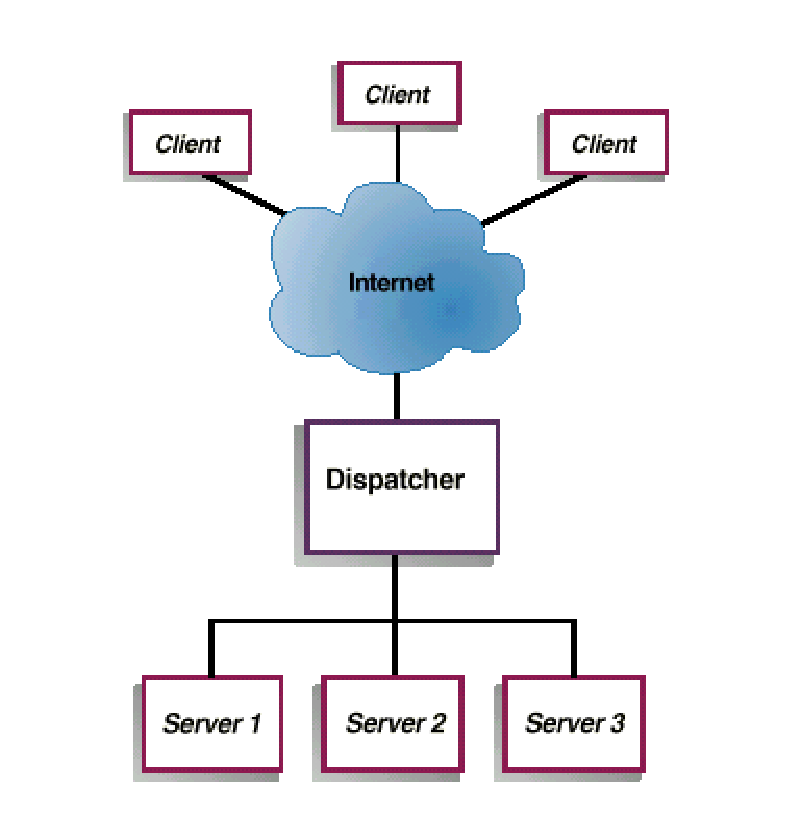
\includegraphics[width=3in]{./rysunki/dispatcher.eps}
\caption{Konfiguracja logiczna modu�u dispatcher}
\label{dispatcher}
\end{figure}

Dispatcher realizuje swoje zadania za pomoc� trzech wewn�trznych komponent�w: Egzekutora, Menad�era i Doradc�w. Egzekutor 
realizuje r�wnowa�enie obci��e�. Dla pakietu wysy�anego w ramach nowego po��czenia mi�dzy klientem a serwerem WEB Dispatcher 
sprawdza, kt�ry z serwer�w mo�e przej�� obs�ug� zlecenia na ��danym przez klienta porcie i adresie klastra. Nast�pnie, dla 
ka�dego takiego serwera, na podstawie zgromadzonych wag okre�laj�cych poziom obci��e� serwer�w, okre�la serwer najmniej 
obci��ony, do kt�rego przekazuje pakiet. Je�li po��czenie ju� istnieje, wtedy bez �adnego przetwarzania pakiet jest natychmiast
wysy�any do tego samego serwera, kt�ry zosta� wybrany podczas inicjalizacji po��czenia. Rozdzia� zlece� mi�dzy serwery bazuje 
na warto�ciach wag wskazuj�cych na mo�liwo�� potencjalnego obci��enia serwera -- np. je�eli jeden serwer ma wag� 2, a drugi ma 
wag� 1, to serwer o wadze 2 powinien dosta� dwa razy wi�cej ��da� ni� ten o wadze 1. Wagi mog� by� ustawiane r�cznie lub przez 
Menad�era. Najcz�ciej do ustawiania wag korzysta si� z Menad�era, kt�ry ustawia wagi automatycznie i w spos�b adaptacyjny, z 
uwzgl�dnieniem aktualnych warunk�w pracy klastra. Menad�er mo�e korzysta� z wewn�trznych licznik�w systemowych oraz z 
informacji dostarczanych przez inne komponenty systemu, takich jak ISS czy WLM. Zarz�dca decyduje kt�ry z serwer�w jest 
najmniej obci��onym poprzez obserwacj� wag serwer�w, kt�re to okresowo analizuje i uaktualnia. Decyzj� jak� serwerowi nada� 
wag� podejmuje opieraj�c si� na czterech parametrach:
\begin{itemize}
\item liczba aktywnych po��cze� realizowanych na ka�dym serwerze TCP;
\item liczba nowych po��cze� na ka�dym serwerze TCP;
\item danych wej�ciowych pochodz�cych od doradc�w;
\item informacji pochodz�cych od narz�dzi monitoruj�cych prac� systemu, takich jak ISS;
\end{itemize}

U�ywanie zarz�dcy jest opcjonalne, ale je�li 
nie jest on u�ywany, r�wnowa�enie obci��enia jest dokonywane przy u�yciu marszrutowania algorytmem wa�onego Round Robina, 
gdzie wagi poszczeg�lnych serwer�w WWW s� nadawane statycznie; 

Aby da� administratorowi wi�ksz� kontrol� nad tym, gdzie kierowane b�d� ��dania r�nego typu pochodz�ce od r�nych grup 
u�ytkownik�w, wprowadzono poj�cie regu� i grup serwer�w im podleg�ych, tj. serwer�w, w�r�d kt�rych b�dzie realizowane 
r�wnowa�enie obci��enia w razie spe�nienia regu�y. Dla Dispatcher'a dost�pne s� regu�y bazuj�ce na: adresie IP klienta, porcie 
klienta, porze dnia, po��czeniach na sekund� dla danego portu, aktywnych po��czeniach dla danego portu. Regu�y daj� mo�liwo�� 
implementacji wysokiej jako�ci us�ug dla wybranych klient�w b�d� w okre�lonej porze dnia. Dost�pna jest tak�e regu�a ,,zawsze 
prawdziwe'', kt�ra oznacza spe�nienie zadanego warunku dla wszystkich przyjmowanych zlece�.
\begin{figure}[h]
\centering
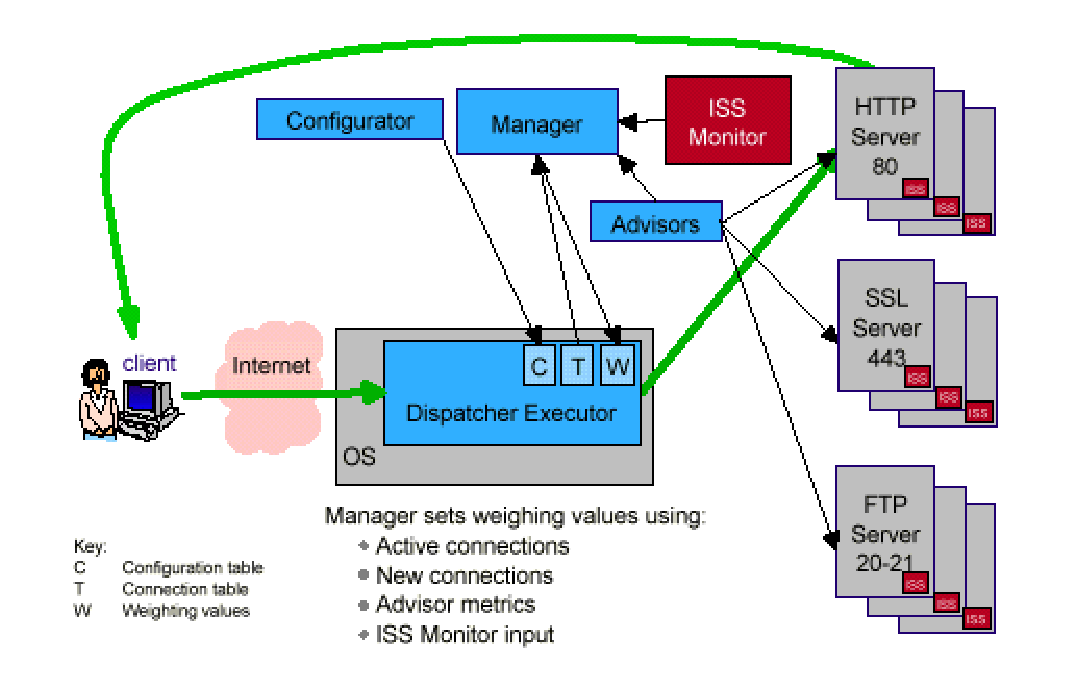
\includegraphics[width=5in]{./rysunki/executor.eps}
\caption{Architektura Network Dispatcher-a}
\label{dispatcher1}
\end{figure}

Zadaniem doradc�w jest zbieranie informacji na temat obci��enia serwer�w. Doradcy sprawdzaj� r�wnie�, czy serwery, na kt�rych 
dokonywane jest r�wnowa�enie obci��e�, funkcjonuj� prawid�owo. Doradcy okresowo otwieraj� po��czenia TCP i wysy�aj� do serwera 
wiadomo�� z ��daniem specyficznym dla danego typu doradcy. Po wys�aniu wiadomo�ci Doradcy czekaj� na odpowied�. Po jej 
otrzymaniu wi�kszo�� Doradc�w szacuje warto�� obci��enia serwera na podstawie czasu, jaki up�yn�� nim serwer zwr�ci� odpowied� 
na ��danie i zg�aszaj� ten czas (w milisekundach) Menad�erowi, aby ten na podstawie tej i innych informacji oszacowa� warto�� 
wag poszczeg�lnych serwer�w. 

Wraz z produktem IBM SecureWay Network Dispatcher dostarczeni s� doradcy: HTTP, FTP, Telnet, NNTP, POP3, SMTP, SSL, WTE, TCP, 
Ping, WLM. Istnieje r�wnie� mo�liwo�� napisania w�asnego doradcy. 

\subsubsection{Komponent Interactive Session Support}

Interactive Session Support (ISS) jest komponentem wsp�pracuj�cym z Domain Name Server (DNS) w jednym z trzech mo�liwych 
tryb�w pracy: DNS--Update, DNS--Replace lub DNS--Ignore. Komponent ten mo�e by� r�wnie� wykorzystany do zbierania informacji na 
temat obci��enia serwer�w, kt�r� nast�pnie przekazuje do Dispatcher'a. W trybie DNS--Update ISS uaktualnia serwer nazw DNS. W 
tym trybie dzia�a on w po��czeniu z serwerem nazw w celu mapowania nazw DNS na adresy IP serwer�w najlepiej nadaj�cych si� do 
obs�ugi danego zadania. W trybie DNS--Replace ISS spe�nia dla ograniczonej podgrupy sieci funkcj� serwera nazw, nie zawiera 
jednak wszystkich funkcji standardowego DNS. W trybie DNS--Ignore, ISS dzia�a w po��czeniu z Dispatcher'em w celu lepszego 
r�wnowa�enia obci��e�.
\begin{figure}[h]
\centering
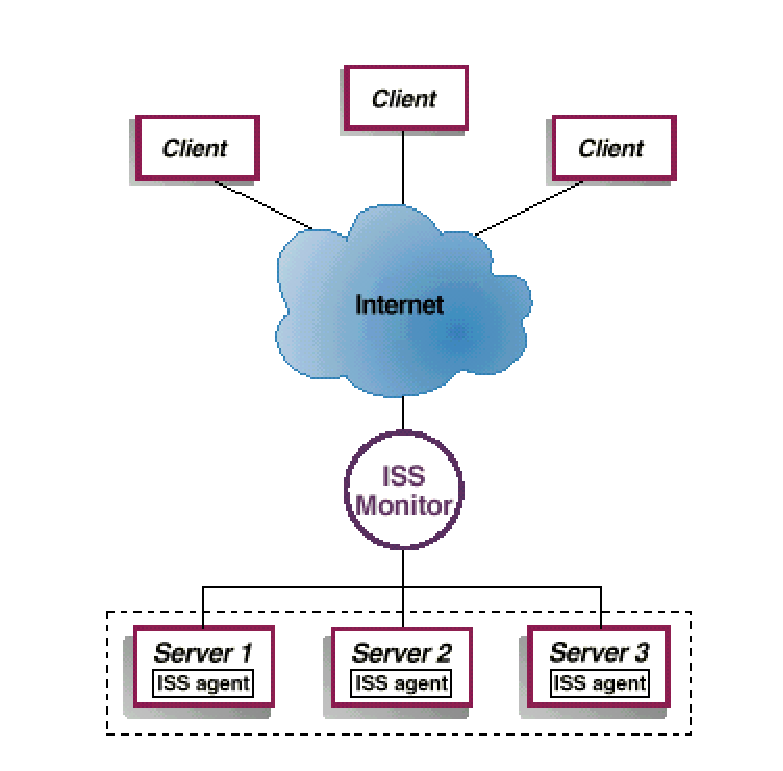
\includegraphics[width=3in]{./rysunki/ISS.eps}
\caption{Konfiguracja logiczna modu�u Interactive Session Support}
\label{ISS}
\end{figure}

Obci��enie na poszczeg�lnych w�z�ach mo�e by� okre�lane poprzez pomiar wykorzystania r�nych zasob�w, takich jak ilo�� wolnej 
pami�ci, u�ycie procesora czy licznik proces�w. ISS pos�uguje si� jedn� z trzech strategii alokacji zlece�: RoundRobin, Best, 
i Statistical RoundRobin.

Przy u�yciu algorytmu RoundRobin, ISS r�wnowa�y obci��enia serwer�w w spos�b klasyczny dla tej strategii. Z danej grupy 
serwer�w ISS wybiera na okre�lony przedzia� czasu jeden serwer, kt�ry b�dzie obci��any w tym przedziale czasu. ISS nie zwraca 
w�wczas uwagi na poziom obci��enia serwera, ale te� nie zaleci serwera, kt�ry niedomaga. Takie podej�cie mo�e funkcjonowa� 
dobrze, pod warunkiem �e obci��enie wywo�ywane przez klient�w jest r�wnomierne. Zalet� tej metody jest brak obci��enia 
serwer�w poprzez procesy pomiarowe. Natomiast jej du�� wad� jest brak elastyczno�ci. Metoda ta mo�e powodowa�, �e np. serwer, 
kt�ry ju� jest bardzo obci��ony, mo�e by� dalej preferowany przez ISS, gdy� nie sko�czy� si� jeszcze przydzielony mu czas.
Stosuj�c strategi� Best, w czasie trwania okre�lonego interwa�u, ISS trasuje ��dania do serwera, kt�ry na pocz�tku tego 
interwa�u mia� najni�szy poziom obci��enia. Tak jak w przypadku poprzedniej metody, korzystaj�cy z niej ISS nie zaleci 
serwera, kt�ry przesta� funkcjonowa�. Ta metoda selekcji sprawdza si� bardzo dobrze dla ka�dego czasu trwania po��cze�, pod 
warunkiem, �e cz�sto�� nowych po��cze� b�dzie relatywnie niska w stosunku do ustawionego interwa�u czasu przydzia�u dla 
pojedynczego serwera. Ta strategia jest przyjmowana domy�lnie przez system.
W strategii Statistical RoundRobin, ISS r�wnowa�y obci��enia na podstawie statystyk obci��enia, kt�re generuje dla wszystkich 
serwer�w. Wykorzystuje te statystyki do budowy profilu najbardziej i najmniej obci��onych serwer�w, a nast�pnie w ci�gu 
trwania interwa�u ,,heartbeat'' rozdziela ��dania pomi�dzy serwery, proporcjonalnie do ich obci��enia. R�wnie� przy u�yciu tej 
metody ISS nie zaleci niedomagaj�cego serwera. Metoda ta sprawdza si� wsz�dzie tam, gdzie wyst�puje du�a cz�sto�� 
kr�tkotrwa�ych po��cze�.

\subsubsection{Komponent Content Base Routing}
 
Komponent CBR mo�e by� skonfigurowany z WTE (Web Traffic Express) dla serwer�w HTTP, lub jako CBR proxy (bez wsp�pracy z WTE)
dla serwer�w IMAP i POP3. CBR wsp�pracuje wesp� z Web Traffic Express, w ten spos�b, �e klient wysy�a ��danie do WTE, kt�ry 
jest skonfigurowany by m�c korzysta� z CBR; CBR musi by� zainstalowany na tej samej maszynie co serwer WTE. WTE wypytuje 
komponent CBR kt�ry serwer ma obs�u�y� ��danie. Gdy CBR otrzyma ��danie pr�buje je dopasowa� do ustawionych regu�. Je�li 
pasuj�, CBR wybiera serwer, z grupy skonfigurowanych do odbierania konkretnego typu ��da�, jednocze�nie r�wnowa��c pomi�dzy 
t� grup� serwer�w obci��enie. 

CBR jest bardzo podobny w strukturze do pakietu Dispatcher. Trzy kluczowe elementy CBR (Egzekutor, Menad�er i Doradcy) 
wsp�pracuj� by zr�wnowa�y� i rozdzieli� przychodz�ce ��dania pomi�dzy serwery w zbli�ony spos�b jak w Dispatcherze. 
Jednak�e w przeciwie�stwie do modu�u Dispatcher -- CBR nie oferuje funkcji zwi�kszonej dost�pno�ci. Jednak�e mo�na po��czy� 
kilka serwer�w CBR i r�wnowa�y� ich obci��enie poprzez serwer ND, kt�ry to mo�e sprawdza� czy �aden z CBR serwer�w nie 
przesta� odpowiada�.

\begin{itemize}
\item CBR z WTE (obs�uguj�cy ruch HTTP)

Komponent CBR wsp�pracuj�c z Web Traffic Express dzia�a jako proxy serwer przekierowuj�c rz�dania klient�w do odpowiednich
serwer�w. Modu� WTE jest proxy serwerem, pozwalaj�cym manipulowa� pami�ci� podr�czn� w celu szybkiego transferu dokument�w
przy niewielkich wymaganiach dotycz�cych przepustowo�ci sieci. CBR za� jest w stanie przefiltrowa� zawarto�� stron WWW 
korzystaj�c ze specyficznych ci�g�w warunk�w nazywanych rolami. CBR daje mo�liwo�� okre�lenia grupy serwer�w, kt�re powinny
przej�� ��danie opieraj�c si� na wyra�eniach regularnych pasuj�cych do zawarto�ci ��dania. Poniewa� CBR pozwala na
,,przywi�zanie'' poszczeg�lnych serwer�w do ka�dego typu ��dania nast�puje zr�wnowa�enie obci��enia serwer�w. CBR potrafi
tak�e wykrywa� kiedy serwer przestaje odpowiada� wy��czaj�c routing ��da� do niego. Zastosowane w module CBR algorytmy
r�wnowa�enia obci��enia s� identyczny z tymi zastosowanymi w komponencie Dispatcher. 

Spos�b dzia�ania CBR: gdy klienckie ��danie jest przesy�ane do WTE proxy nast�puje tu korelowanie zawarto�ci ��dania
z regu�ami zdefiniowanymi w module CBR. Je�li zbi�r regu� pasuje do zawarto�ci ��dania jeden z serwer�w ,,zwi�zanych'' z 
obs�ug� tego typu ��da� zostaje wybrany do przyj�cia ��dania. Wtedy WTE jako proxy serwer przekierowuje do wybranego serwera 
��danie. Jak wida� modu� WTE musi by� uruchomiony zanim CBR zostanie skonfigurowany, poniewa� dzia�a on jako podproces WTE.
Oczywi�cie oba modu�y musz� znajdowa� si� na tej samej maszynie.

Oznacza to podzia� farmy serwer�w na cz�ci realizuj�ce odpowiedni typ ��da�. Taki podzia� jest przezroczysty dla klienta. 
Mo�na np. podzieli� witryn� na dwie cz�ci -- kilka serwer�w realizuj�cych tylko ��dania CGI, a pozosta�e reszt� ruchu HTTP.
Pozwala to na realizacj� intensywnie przetwarzanych skrypt�w CGI w spos�b nie koliduj�cy z prac� reszty serwer�w WWW 
obs�uguj�cych normalny ruch HTTP -- co oznacza dla klienta lepszy og�lny czas odpowiedzi. W ten spos�b komputery o wi�kszej
mocy obliczeniowej mo�na przeznaczy� na obs�uge normalnego ruchu bez kosztownego upgradu wszystkich komputer�w.
\begin{figure}[h]
\centering
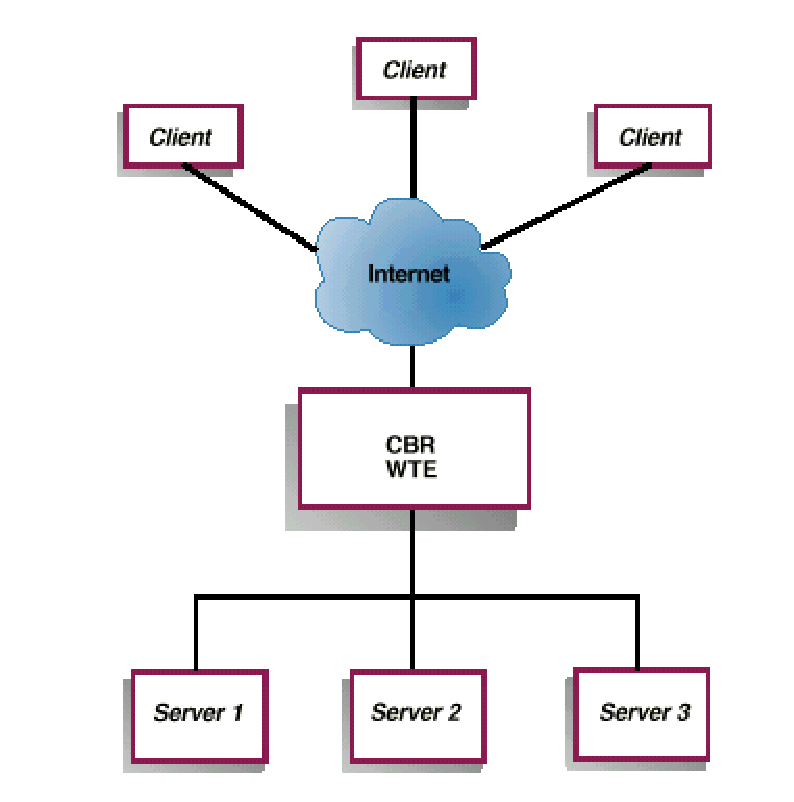
\includegraphics[width=3in]{./rysunki/CBR-WTE.eps}
\caption{Konfiguracja logiczna modu�u Content Base Routing (wraz z WTE)}
\label{CBR}
\end{figure}


Inn� mo�liwo�ci� podzia�u serwera WWW jest bezpo�rednie przekierowanie klient�w, kt�rzy chc� dosta� si� do stron wymagaj�cych
rejestracji, do jednego typu serwer�w, a reszt� do pozosta�ych. Wtedy obs�ug� stron wymagaj�cych rejestracji zajmuj� si�
np. komputery o wi�kszej mocy obliczeniowej i klienci, kt�rzy s� ju� zarejestrowani maj� lepszy czas odpowiedzi ni� inni. 

Wybieraj�c role dokonuj�ce r�wnowa�enia obci��enia nale�y sprawdzi� czy wszystkie ��dania do klastra WWW posiadaj� role, 
na podstawie ktorych mo�na wybra� serwer. Je�li tak nie jest, tzn. je�li przychodz�ce ��danie nie pasuje do �adnej roli, klient
otrzyma komunikat o b��dzie pochodz�cy z WTE. Najprostszym rozwi�zaniem jest stworzenie roli zawsze prawdziwej z bardzo 
wysokim priorytetem i ,,przywi�zanie'' jej do osobnej grupy serwer�w.

\item CBR proxy (obs�uguj�cy ruch IMAP i POP3)

CBR bez WTE mo�e by� proxy wybieraj�cym odpowiedni serwer opieraj�c si� na ID u�ytkownika i ha�le. Nie wspiera wtedy opartego
na rolach r�wnowa�enia obci��e�.
\end{itemize}

\subsection{Content Base Routing -- konfiguracja}

CBR mo�e zosta� skonfigurowany jako proxy dla us�ug opartych o protoko�y POP3 lub IMAP -- dzia�a wtedy bez wsp�pracy
z modu�em WTE, lub tez jako narz�dzie r�wnowa��ce obci��enie ruchu HTTP -- systemem proxy jest wtedy WTE  \cite{NDUsersGuide}.

Modu� ten mo�na skonfigurowa� za pomoc� linii komend lub z pomoc� graficznego interfejsu u�ytkownika
(\emph{GUI}). Modu� Content Base Routing jest bardzo podobny w architekturze do Dispatchera. Sk�ada si� on z trzech
funkcjonalnych cz�ci:
    \begin{itemize}
    \item Egzekutor -- zajmuje si� r�wnowa�eniem obci��enia zapyta� klienckich. Jest zawsze uruchomiany je�li CBR
    jest w u�yciu;
    \item Menad�er -- ustala wagi dla poszczeg�lnych serwer�w opieraj�c si� na:
        \begin{itemize}
        \item wewn�trznych licznikach Egzekutora;
        \item informacjach zbieranych z serwer�w przez doradc�w;
        \item informacjach z program�w monitoruj�cych prace systemu, takich jak ISS czy WLM.
        \end{itemize}
        Korzystanie z menad�era jest opcjonalne. Jednak�e gdy jest on nieu�ywany -- r�wnowa�enie obci��enia jest
        realizowane za pomoc� algorytmu statycznego Wa�onego Round--Robin opartego na domy�lnych wagach, a
        doradcy nie b�d� wtedy dost�pni.
    \item Doradcy -- wypytuj� serwery oraz analizuj� dane o ich stanie, by nast�pnie z tak spreparowanych danych
    Menad�er ustali� odpowiednie wagi. Korzystanie z Doradc�w jest r�wnie� opcjonalne, a typowej konfiguracji wr�cz
    mo�e nie by� potrzebne, jednak�e mimo to poleca si� z nich korzysta�.
    \end{itemize}

Wszystkie trzy cz�ci (Egzekutor, Menad�er oraz Doradcy) wsp�pracuj� ze sob� w celu rozbalansowania i
rozpropagowania przychodz�cych ��da� pomi�dzy serwery.

Aby skonfigurowa� wst�pnie CBR, mo�na pos�u�y� si� jedna z czterech dost�pnych metod:
    \begin{enumerate}
    \item Linii komend;
    \item Skrypt�w konfiguracyjnych;
    \item Graficznego interfejsu u�ytkownika;
    \item Konfiguracyjnego wizarda.
    \end{enumerate}

\subsubsection{Konfiguracja maszyny CBR}

Aby moc konfigurowa� CBR, nale�y mie� status root--a w systemie. Nale�y tak�e zna� adresy ka�dego z
konfigurowanych klastrow serwer�w. Pojedynczy adres IP jest tu u�ywany jako jeden adres dla ca�ego klastra.
Zanim jednak�e przeprowadzi si� konfiguracje i uruchomienie modu�u CBR -- musi by� ju� skonfigurowany i
uruchomiony WTE. Konfiguracje wykonuje si� w takiej kolejno�ci (konfiguracja dotyczy tylko ruchu HTTP):
    \begin{enumerate}
    \item Uruchomienie WTE
    \item Po uruchomieniu WTE, nale�y zdefiniowa� klaster WWW, oraz ustawi� specyficzne dla tego
    klastra opcje. Do zdefiniowania klastra oraz opcji s�u�y komenda:\\
    
    cbrcontrol cluster set \emph{cluster opcja warto��}\\
    
    \item Nast�pnym krokiem jest zdefiniowanie port�w ustalenie ich opcji. Wykonuje si� to komend�:\\
    
    cbrcontrol port set \emph{cluster:port opcja warto��}\\
    
    \item Definiowanie poszczeg�lnych komputer�w nale��cych do serwera:\\
    
    cbrcontrol server add \emph{cluster:port:server}\\
    
    gdzie \emph{server} jest nazw� symboliczn� pojedynczego komputera w klastrze, lub jego adresem IP;
    \item Nast�pnym krokiem jest konfiguracja regu� CBR. Jest to krok kluczowy w konfiguracji CBR przy ruchu po protokole HTTP
    regu�y (role) definiuj� jak zadanie URL zostanie przes�ane do jednego lub wi�kszej ilo�ci serwer�w. Te specyficzne
    regu�y nazywaj� si� regu�ami zawartosci\footnote{\emph{and. -- content rule}}. Aby zdefiniowa� regu��
    korzysta si� z nast�puj�cej komendy:\\
    
    cbrcontrol rule add \emph{cluster:port:rule} type content pattern=\emph{pattern}\\
    
    gdzie warto�� \emph{pattern} jest wyra�eniem regularnym, kt�re b�dzie por�wnywane za ka�dym razem jak
    nadejdzie ��danie od klienta.
    \item Nast�pnie nale�y doda� poszczeg�lne serwery obs�uguj�ce regu�y zawarto�ci. Gdy wyst�puje dopasowanie
    pomi�dzy ��danym URL, a regu�� zawarto�ci zostaje wybrany najlepszy z serwer�w obs�uguj�cych ten typ
    ��da�. Aby wykona� takie dopasowanie -- regu�a dopasowania--serwer obs�uguj�cy wykonuje si� polecenie:\\
    
    cbrcontrol rule useserver \emph{cluster:port:rule server}\\
    
    \item Uruchomienie Menad�era (opcjonalne):\\
    
    cbrcontrol manager start\\

    \item Uruchomienie Doradc�w (opcjonalne):\\

    cbrcontrol advisor start http \emph{port}

    \item Ostatnim krokiem jest skonfigurowanie Doradc�w, aby ich informacje bra�y udzia� w decyzjach r�wnowa�enia
    obci��enia.
    
    \end{enumerate}

\subsubsection{Konfiguracja LB opartego na regu�ach}

Wykorzystuj�c do r�wnowa�enia obci��enia WTE wraz z modu�em CBR -- mo�na rozdziela� ruch sieciowy
wykorzystuj�c nast�puj�ce typy regu�:
    \begin{itemize}
    \item Adres IP klienta; jest to sytuacja, gdy wymaga si� alokacji zasob�w w zale�no�ci od tego sk�d przychodzi
    zadanie. Mo�na za�o�y�, ze z pewnych adres�w (od klient�w) wymagamy by zadania nie by�y realizowane, zatem
    przygotowuje si� regule i nie dodaje do �adnego serwera -- wtedy okre�leni klienci nie b�d� obs�ugiwani
    (wyst�pi b��d). np.:\\

    ndcontrol rule add 9.67.131.153:80:ni type ip beginrange 9.0.0.0 endrange \
    9.255.255.255\\

    taka regu�a oznacza, ze klienci z domeny IBM--a nie osi�gn� serwera CBR;        
    \item Godzina po��czenia; tak� regu�� wykorzystuje si� g�ownie przy okre�lonych planach obs�ugi obci��e�.
    W przypadku gdy witryna produkcyjna otrzymuje pewna grup� ��da� o pewne dokumenty w okre�lonym
    (i sta�ym) czasie ka�dego dnia -- mo�na tylko dla tych ��da� wyznaczy� osobne serwery; mo�e to by� tak�e
    przydatne w przypadku gdy w godzinach nocnych (najmniejszy ruch) -- niekt�re maszyny z powodu wykonywania
    backupu powinny by� wy��czone z realizacji ��da�;
    \item Ilo�� po��cze� na sekund�, na port; (dzia�a tylko podczas uruchomionego Menad�era) mo�na wykorzystywa�
    np. w przypadku: \emph{if po��cze� na sekund� na porcie 80 > 100 then u�yj te dwa serwery}, \emph{if po��cze�
    na sekund� na porcie 80 > 2000 u�yj te 8 serwer�w};
    \item Ca�kowita ilo�� aktywnych po��cze� na porcie; (wym�g jak wy�ej -- Menad�er musi by� uruchomiony);
    Jest to regu�a potrzebna w przypadku gdy wiadomo kiedy serwer b�dzie np. prze�adowany (przy ilu po��czeniach)
    Je�li np. wiadomo, ze serwer nie jest w stanie przyj�� i zrealizowa� naraz wi�cej niz. 250 jednoczesnych po��cze�
    tworzy si� regu��:\\

    ndcontrol rule add 130.40.52.153:80:pool2 type active beginrange 250 endrange 500\\

    Wtedy do tak stworzonej regu�y do pojedynczego serwera mo�na doda� nast�pne maszyny, kt�re w przypadku
    wi�kszej ilo�ci po��cze� zostan� w��czone w podejmowanie ��da�;
    \item regu�a zawsze prawdziwe; Regu�a ta jest zawsze spe�niona -- chyba ze serwery z kt�rymi jest zwi�zana
    nie pracuj�; przydaj� si� w przypadku gdy nie chcemy aby jakikolwiek klient dosta� zwrot w postaci b��du
    zadania dokumentu (od WTE);
    \item Zawarto�� zadania; (jest to regu�a dost�pna tylko z poziomy modu�u CBR); regu�a wykorzystywana
    w przypadku dystrybucji ��da� w zale�no�ci od zawarto�ci zadania; np. gdy potrzeba aby jedna grupa serwer�w
    obs�ugiwa�a zadania \emph{cgi--bin}, inna grupa obs�ugiwa�a media strumieniowe (np. real media), za� trzecia wszystkie
    pozosta�e wtedy wzorcem pierwszej z regu� 
    b�dzie �cie�ka do katalogu cgi--bin, drugiej do plik�w strumieniowych, a trzeciej regu�a zawsze prawdziwe;
    nast�pnie nale�y tylko przyporz�dkowa� regu�y do odpowiadaj�cych im grup serwer�w;
        \begin{description}
        \item[Typy regu� dla CBR]\

        sk�adnia wzorc�w regu� wygl�da nast�puj�co: w regule (wzorcu)  nie mo�e by� �adnych przerw (spacji)
        ani znak�w specjalnych:
            \begin{description}
            \item[*] -- odpowiada 0 do x wyst�pienia dowolnych znak�w;
            \item[)(] -- u�ywane do grupowania logicznego;
            \item[\&] -- logiczne AND;
            \item[|] -- logiczne OR;
            \item[!] -- logiczne NOT;
            \end{description}
        Zarezerwowane s�owa (zawsze nast�puje do nich przyporz�dkowanie w postaci znaku r�wno�ci):
            \begin{description}
            \item[client] -- adres IP klienta;
            \item[url] -- URL w zadaniu;
            \item[path] -- sekcja �cie�ka URL--a;
            \item[protocol] -- sekcja protok�u URL--a;
            \item[refer] -- \emph{quality of service}
            \end{description}
        Poni�ej znajduj� si� przyk�ady:\\

        \emph{url=http://*/*.gif}\\

        \emph{client=9.32.*}\\

        \emph{!(path=*.jpeg)}\\

        \emph{(path=index/*.gif \& protocol=httpd) | (client=9.1.2.3)}       
        \end{description}
    \end{itemize}

Wszystkie regu�y posiadaj� nazw�, typ, priorytet, pocz�tkowy zakres dzia�ania, ko�cowy zakres dzia�ania oraz
grup� obs�uguj�cych serwer�w. Dodatkowo, regu�a zawarto�ci w komponencie CBR posiada zwi�zane ze sob�
wyra�enie regularne. Regu�y s� wykorzystywane w kolejno�ci ich priorytet�w. Regu�y z niskim priorytetem s�
realizowane wcze�niej. Innymi s�owy, regu�a z priorytetem 1 jest wykorzystywana przed regu�a o priorytecie 2.
Pierwsza poprawnie dopasowana regu�a zostaje wykorzystana (reszta ju� nie jest pr�bkowana).

Aby regu�a zosta�a spe�niona musza by� spe�nione naraz dwa warunki:
    \begin{enumerate}
    \item Predykat regu�y musi by� prawdziwy. Co oznacza, ze warto�� por�wnana musi znajdowa� si� pomi�dzy
    warto�ciami pocz�tkowa i ko�cowa, lub zawarto�� zadania musi pasowa� do wyra�enia regularnego
    wyspecyfikowanego w wzorcu\footnote{ang. \emph{pattern}}. Dla regu� o typie ,,zawsze prawdziwy''
    regu�a jest zawsze spe�niona (bez warunk�w);
    \item Je�li istniej� serwery zwi�zane do poszczeg�lnych regu�, co najmniej jeden z nich musi by� dost�pny do
    odebranie zadania.
    \end{enumerate}

W przypadku, gdy nie ma serwer�w dla kt�rych konkretna regu�a nie mog�aby by� spe�niona -- zadanie zostaje
porzucone, a CBR zwr�ci do serwera proxy (WTE) komunikat b��du. Je�li za� �adna z regu� nie mo�e zosta�
spe�niona -- jak wy�ej -- CBR zwr�ci do WTE komunikat b��du.

\subsection{Narz�dzie do test�w -- Astra Load Runner}

Narz�dziem testowym w wykonanym projekcie by�o oprogramowanie firmy Mercury Interactive\footnote{http://www.merc-int.com}
-- Astra Load Runner. Jego wyb�r by� spowodowany szerokim wachlarzem mo�liwo�ci testowych, obs�ugiwanych protoko��w oraz
mo�liwo�ci dokonywania analiz i wizualizacji rezultat�w. Poni�ej znajduje si� kr�tka charakterystyka tego progrmau:

LoadRunner jest narz�dziem do test�w wydajno�ciowych, dzi�ki kt�rym mo�na sprawdzi� wydajno�� i skalowalno�� systemu webowego.
Jest on w stanie generowa� dziesi�tki, setki czy nawet tysi�ce jednoczesnych u�ytkownik�w, umo�liwiaj�c w ten spos�b wykrycie 
wszystkich s�abych, b�d� niewydajnych miejsc w naszym systemie. W czasie trwania testu dost�pne s� r�norakie 
monitory, wy�wietlaj�ce ca�y czas wszystkie interesuj�ce parametry systemu funkcjonuj�cego pod obci��eniem. Dzi�ki 
tym wbudowanym monitorom mo�na np.:  na bie��co �ledzi� czasy odpowiedzi wszystkich serwer�w, czasy wykonywania si� danych 
transakcji czy szybko�� transferu danych w sieci z podzia�em na segmenty.

Wszyscy u�ytkownicy generowani przez LoadRunnera kontrolowani s� z jednego centralnego modu�u zwanego kontrolerem. Testuj�c 
system pod obci��eniem mo�na symulowa� r�ne numery IP klient�w, r�ne przegl�darki internetowe oraz r�ne 
szybko�ci ��czy internetowych, ca�y czas jednocze�nie monitoruj�c zachowanie naszego obci��anego systemu.
Dane Techniczne Narz�dzia:
\begin{description}
\item[Wspierane protoko�y typu klient/serwer]\
	\begin{itemize}
	\item Oracle UPI
	\item Oracle OCI
	\item ODBC
	\item MS-SQL Server
	\item Sybase ctlib
	\item Sybase dblib
	\item Informix I-Net
	\item DB2 CLI
	\item Tuxedo (including compression mode)
	\item RTE
	\item CORBA
	\item COM/DCOM
	\item WinSocket
	\end{itemize}
\item[Wspierane protoko�y ERP]\
	\begin{itemize}
	\item SAP R/3
	\item PeopleSoft (2-tier i Tuxedo-based)
	\item Oracle Applications
	\item Siebel
	\item Baan
	\end{itemize}
\item[Wspierane protoko�y internetowe]\
	\begin{itemize}
	\item Streaming (Real Audio and Real Video)
	\item MS Media
	\item iMode
	\item VoiceXML
	\item LDAP
	\item WAP--HTTP
	\item WAP--Gateway
	\item HTTP
	\item HTTPS (SSL)
	\item Digital Certificates
	\item RMI
	\item FTP
	\item POP3
	\item Winsock
	\item SMTP
	\end{itemize}
\item[Wspierane systemy Legacy]\
	\begin{itemize}
	\item 3270 Terminals (Mainframe)
	\item 5250 Terminals (AS/400)
	\item VT    Terminal   (DEC)
	\item X Window Applications
	\end{itemize}
\item[Tworzenie test�w wydajno�ciowych:]\
	\begin{itemize}
	\item Mo�liwo�� prze��czania rodzaju nagrywanego protoko�u w trakcie rejestracji jednego skryptu;
	\item Narz�dzie automatycznie generuje skrypty test�w obci��eniowych, oparte na operacjach biznesowych wykonywanych na 
	testowanej aplikacji;
	\item Narz�dzia do automatycznej parametryzacji skrypt�w pozwalaj� na szybk� i wydajn� obr�bk� stworzonego testu;
	\item Przypisywanie r�nych numer�w IP do poszczeg�lnych symulowanych u�ytkownik�w daje du�e mo�liwo�ci w tworzeniu 
	scenariuszy testowych;
	\item Automatyczna kontrola zawarto�ci danych w czasie test�w wydajno�ciowych, stanowi�ca jednocze�nie kontrol� funkcjonaln�;
	\item Automatyczne korelowanie dynamicznie zmieniaj�cych si� danych przy nagrywaniu i odtwarzaniu skrypt�w;
	\item Korelacja zapyta� Oraclowych, polegaj�ca na mo�liwo�ci przechwytywania danych pobieranych z bazy i wykorzystywaniu ich w 
	dalszej cz�ci skryptu;
	\item Emulacja po��czenia modemowego o r�nej przepustowo�ci;
	\item Kreator scenariuszy testowych, daj�cy mo�liwo�� szybkiego i efektywnego tworzenia ca�ych scenariuszy testowych.
	\end{itemize}

\item[Kontrolowanie test�w wydajno�ciowych]\
	\begin{itemize}
	\item Automatyczna kontrola i synchronizacja wszystkich symulowanych u�ytkownik�w z jednego centralnego punku kontroli;
	\item Monitorowanie w czasie rzeczywistym wszystkich parametr�w systemu;
	\item �atwy w u�yciu graficzny interfejs, umo�liwiaj�cy tworzenie, uruchamianie, monitorowanie i analizowanie wynik�w testu;
	\item Jeden wsp�lny punk kontroli dla ca�ego testu z mo�liwo�ci� uruchamiania u�ytkownik�w na systemach Windows i Unix.
	\end{itemize}

\item[Pomiary i kontrola wydajno�ci]\
\begin{itemize}
	\item Mo�liwo�� pomiaru i kontroli czasu wykonywania si� mierzonych transformacji w zadanych kryteriach lub od ,,zapytania -- 
	do odpowiedzi'' tzn. ��cznie z czasem przetwarzania klienta, serwera i sieci komputerowej;
	\item Mo�liwo�� wygenerowania dedykowanego obci��enia serwera, powielaj�c zarejestrowan� transmisj� po konkretnym protokole;
	\item Pomiar parametr�w systemu operacyjnego dzia�aj�cego na obci��anym serwerze, daj�cy mo�liwo�� znalezienia s�abych punkt�w 
	konfiguracji i zasobach systemu operacyjnego;
	\item Pomiar parametr�w sprz�towych maszyny b�d�cej obci��anym serwerem, daj�cy mo�liwo�� znalezienia s�abych i niewydolnych 
	punk�w w konfiguracji sprz�towej testowanej maszyny;
	\item Mo�liwo�� pomiaru czas�w wykonywania si� transakcji zdefiniowanych przez testera.
	\end{itemize}
\item[Analiza i kontrola wynik�w, dost�pne monitory:]\
	\begin{itemize}
	\item Server Resource Monitor ( NT, Unix, Linux) -- pozwala na kontrolowanie zasob�w sprz�towych maszyn b�d�cych 
	testowanymi serwerami;
	\item Network Delay Monitor -- pozwala na kontrolowanie czas�w odpowiedzi i realizowania si� monitorowanych transakcji we 
	wszystkich segmentach sieci obci��anego systemu;
	\item SNMP Monitor -- pozwala na kontrolowanie przep�ywu danych pomi�dzy poszczeg�lnymi elementami aktywnymi sieci jak: 
	Routery, Huby, Bridge;
	\item WebSphere, ColdFusion, SilverStream, BroadVision, ATG Dynamo, GemStone/J, Ariba Buyer, WebLogic, MS ASP, iPlanet -- 
	monitory serwer�w aplikacji internetowych, posiadaj�ce specjalne wsparcie dla ka�dego z nich;
	\item EJB, TUXEDO -- kontroluje i monitoruje wszystkie parametry systemu opartego na aplikacjach TUXEDO i EJB;
	\item MS IIS, Netscape, Apache -- monitory serwer�w webowych;
	\item RealServer, Windows Media Server -- monitory do kontrolowania technologii strumienowych;
	\item COM/CORBA -- monitory do kontrolowania i badania technologii rozproszonych;
	\item ORACLE, SQLServer -- monitory do �ledzenia i badania wydajno�ci serwer�w baz danych, zawieraj�ce specjalne wsparcie i 
	integracje z tym technologiami.
	\end{itemize}

\item[Wirtualni u�ytkownicy s� odtwarzani na systemach:]\
	\begin{itemize}
	\item Windows NT
	\item Sun Solaris
	\item HP--UX
	\item IBM AIX
	\item Linux
	\end{itemize}

\end{description}



\section{Projekt systemu do zarz�dzania wielokomputerowymi serwerami WWW w oparciu o IBM SecureWay Network Dispatcher}

Ca�o�� zadania polega�a na stworzeniu jednej architektury systemu WWW kt�rego witryna zawiera�aby oko�o 60\% zawarto�ci
w postaci stron dynamicznych (wype�nianych danymi pochodz�cymi ze znajduj�cego si� w uk�adzie serwera baz danych) generowanych
on line. Jednak�e rozdysponowanie obci��enia pomi�dzy poszczeg�lnymi elementami serwisu WWW by�o realizowane na trzy sposoby: 
statycznie, dynamicznie oraz w zale�no�ci od typu nadchodz�cych do serwera ��da�. Taka architektura mia�a da� odpowied� na 
pytanie -- jak zaprojektowa� sytem WWW obs�uguj�cy strony generowane dynamicznie w mo�liwie najbardziej efektywny spos�b.

\subsection{Architektura}

W eksperymencie wykorzystano lokaln� sie� komputerow� z�o�on� z jednego segmentu sieci FastEthernet. W jego sk�ad wchodzi�y
komputery, na kt�rych zainstalowane by�o oprogramowanie generuj�ce obci��enie dla klastera serwer�w WWW (razem dziewi�� sztuk)
pracuj�cych pod kontrol� systemu Windows NT 4.0 Server (Service Pack 6a).
 
\begin{figure}[h]
\centering
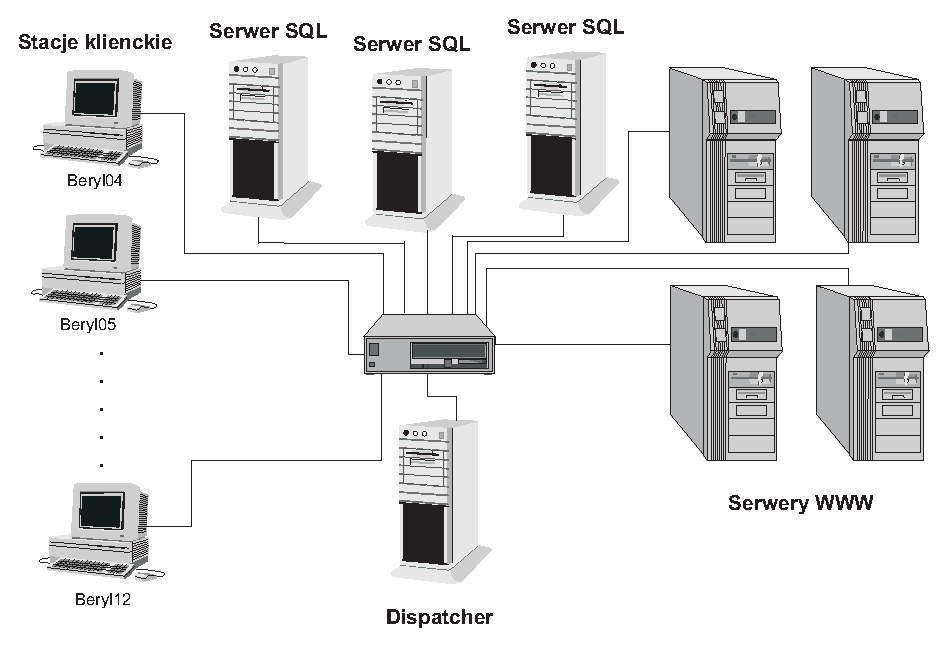
\includegraphics[width=14cm]{./rysunki/komputerki.eps}
\caption{Architektura segmentu sieci testowej.}
\label{architektura}
\end{figure}
Ka�dy komputer wyposa�ony by� w procesor Intel 
Celeron 300 MHz, 96 MB pami�ci SDRAM, dysk twardy o pojemno�ci 3 GB oraz kart� sieciow� 3COM EtherLink XL (10/100 Mbps). 
P�yta g��wna ka�dego komputera zbudowana by�a w oparciu o chipset Intel 430 LX. Komputery te posiada�y adresy IP z zakresu 
156.17.130.69 -- 156.17.130.79 i nazwy odpowiednio Beryl04 -- Beryl12. Na komputerach tych zainstalowane by�o oprogramowanie
Astra LoadRunner firmy Mercury Interactive. Komputery o identycznej architekturze stanowi�y serwery baz danych: beryl01 (IP = .66), beryl02 (IP = .67), beryl03 (IP = .68).
Zainstalowano na nich MS SQL server w wersji 7.0 (wersja 120 dniowa) wraz z baz� testow�.

Poza wy�ej wymienionymi komputerami PC pod��czony by�y badany klaster serwer�w WWW. Sprz�tow� platform� serwer�w by�y 
komputery IBM RS 6000 43P Model 260 pracuj�ce pod kontrol� systemu operacyjnego AIX 4.3.3. Ka�dy z tych komputer�w posiada� 
256 MB pami�ci RAM, dysk twardy UW SCSI o pojemno�ci 4.3 GB oraz zintegrowan� kart� sieciow� IBM 10/100 Mbps. ,,Sercem'' tej 
serii komputer�w RS 6000 jest procesor RISC PowerPC Power3 taktowany cz�stotliwo�ci� 200 Mhz. Trzy z wykorzystywanych maszyn 
posiada�y jeden taki procesor a dwa wyposa�one by�y w dwa procesory po��czone w architekturze SMP. Na ka�dym z badanych 
serwer�w zainstalowane by�o oprogramowanie serwera WWW Apache for AIX. Poszczeg�lne komputery RS 6000 posiada�y adresy IP z 
zakresu 156.17.130.45 -- 156.17.130.49 i nazwy odpowiednio akwamaryn (RS/6000 dwuprocesorowy), szafir (dwuprocesorowy), 
opal01 -- opal03 (jednoprocesorowe). Jedna maszyna dwuprocesorowa (szafir) pos�u�y�a do 
rozpropagowania obci��enia (dispatcher+CBR i WTE), druga pos�u�y�a do obs�ugi ��da� o statyczne
pliki HTML, za� pozosta�e maszyny obs�ugiwa�y dynamicznie generowane (poprzez skrypty PHP) strony,
w ten spos�b, �e ka�dy z opali pobiera� dane z bazy danych poszczeg�lnych beryli (opal01--beryl01,
 opal02--beryl02 i opal03--beryl03).

Wszystkie komputery by�y po��czone ze 100Mbps switchem OmniS/R-5 firmy Alcatel. R�wnie� wyj�cie na Swiat by�o realizowane z
t� szybko�ci�. 

Konstrukcja zarz�dzanego, wielokomputerowego systemu WWW by�a bardzo z�o�ona. Sk�ada�a si� z 
nast�puj�cych element�w:
\begin{enumerate}
\item Instalacja i konfiguracja switcha OmniSwitch/Router firmy Alcatel;
\item Instalacja i konfiguracja dispatchera z modu�em CBR. W sk�ad tej cz�ci wesz�y: 
\begin{itemize}
\item instalacja systemu AIX w wersji 4.3.3 oraz jego update do wersji 4.3.3.0.8 (niezb�dne pliki
zosta�y �ci�gni�te z odpowiedniej strony firmy IBM;
\item instalacja wirtualnej maszyny (VM) Javy w wersji 1.3.0;
\item instalacja oprogramowania IBM WebSphere Edge Server 1.0.3  wraz z 60--dniow� licencj�;
\item skonfigurowanie WTE jako \emph{reverse proxy } o adresie URL: www1.ists.pwr.wroc.pl, kt�ry
przekierowywa� adresy URL do serwer�w: opal01, opal02, opal03 i akwamaryn, w ten spos�b, aby
��dania o statyczne pliki HTML zosta�y skierowane do serwera akwamaryn, za� ��dania o dynamicznie
generowane strony z rozszerzeniami: .PHP, .PHP3 i PHP4 zosta�y rozpropagowane na pozosta�e
trzy maszyny;
\end{itemize}
\item Instalacja i konfiguracja oprogramowania dodatkowego na poszczeg�lne serwery WWW i 
dispatchera tzn. HTTP Server Apache w wersji 1.3.19, kompilator C i C++ w postaci gcc w wersji
2.95.3 oraz j�zyka skryptowego PHP w wersji 4.0.6;
\item Instalacja i konfiguracja Windows NT 4.0 Server wraz z Service Pack 6.0 na dwunastu
laboratoryjnych komputerach PC;
\item Instalacja i konfiguracja Microsoft SQL Serwera w wersji 7.0 na serwerach baz danych oraz
instalacja bazy testowej;
\item Instalacja oprogramowania do test�w na pozosta�ych komputerach; przygotowanie testu;
\item przygotowanie witryny WWW do test�w;
\end{enumerate}

\subsection{Algorytmy i metody}
Poni�ej znajduj� si� opisane trzy powsta�e modele. W ka�dym z nich program komputer (RS/6000) wraz z zainstalowanym programem 
IBM SecureWay Network Dispatcher stanowi uk�ad rozdysponuj�cy ��daniami. 

\subsubsection{Information less -- modu� dispatcher + Round Robin}

Sam Dispatcher nie ma mo�liwo�ci pracy w statycznym algorytmie Round Robin, jednak�e (jak napisano powy�ej, w charakterystyce 
oprogramowania) mo�na pos�ugiwa� si� modu�em Dispatcher z wy��czonym modu�em Zarz�dcy oraz z og�rnie nadanymi wagami. W tym
przypadku, pomimo niehomogenicznego �rodowiska nadano wszystkim elementom klastra WWW wagi r�wne jeden. W tej sytuacji komputer
z zainstalowanym dispatcherem r�wnomiernie (bez jakiejkolwiek analizy) propagowa� ��dania do poszczeg�lnych komputer�w.

W tym przypadku dost�p do bazy danych m�g� by� realizowany z dowolnego komputera (serwera WWW).

\subsubsection{Server info aware -- modu� dispatcher + Weighted Round Robin}

W por�wnaniu do poprzedniego przypadku w tym u�yto Dispatchera z uruchomionym modu�em zarz�dcy. Wtedy te� realizowany by�
algorytm Wa�ony Round--Robin. Wagi nadawane by�y dynamicznie tzn. w zale�no�ci od obci��enia poszczeg�lnych komputer�w -- 
serwer�w WWW. 

W tym jak i w powy�szym przypadku dost�p do bazy m�g� by� r�wnie� realizowany z dolwolnego z serwer�w WWW.

\subsubsection{Client info aware -- modu� CBR + WTE}

By� to najbardziej z�o�ony przypadek. Ka�dy pakiet by� analizowany pod wzgl�dem typu zawarto�ci oraz pod wzgl�dem jego 
obecno�ci w keszu komponentu WTE. CBR zosta� tak skonfigurowany aby rozpoznawa� URL z zawartym w nim wyrazem .php 
(identyfikuj�cym plik HTML z zawartym kodem PHP dost�pu do bazy). Pozwoli�o to na rozdzdzia� zapyta� na ��dania o pliki
statyczne (te by�y rozsy�ane go trzech jednoprocesorowych maszyn RS/6000), za� te ��dania o pliki, kt�rych cz�� by�a
generowana dynamicznie by�y przekazywane na dwuprocesorowy serwer, kt�ry komunikowa� sie (tylko on) z serwerem baz danych.
Taka konfiguracja pozwoli�a rozdysponowa� zar�wno obci��enie jak i typ po��cze�.

\subsection{Metodologia testowania}

Celem testowania powsta�ego systemu do zarz�dzania wielokomputerowym serwerem WWW
jest zbadanie wydolno�ci takiego systemu -- tzn. jego wydajno�ci w sytuacji
maksymalnego obci��enia, czyli tak�e mo�liwo�ci odpowiedzi na klienckie 
��danie w takiej sytuacji. Zamierzeniem testowania jest odpowied� na 
pytanie jak obci��enie jest r�wnowa�one pomi�dzy poszczeg�lnymi cz�ciami
sk�adowymi systemu, w zale�no�ci od algorytmu dysypacji obci��enia
(Round--Robin, Weighted Round--Robin oraz rozproszenie oparte na CBR), oraz
jaki dany algorytm ma wp�yw na LB.

Testowanie zaprojektowanego rozproszonego serwera WWW polega�o na pomiarze
wydajno�ci tak wej�ciowej jak i wyj�ciowej ca�ego systemu jak i poszczegolnych
jego sk�adowych (poszczeg�lnych serwer�w WWW, serwera baz danych i dispatchera).

Celem testowania by�o zbadanie maksymalnej wydajno�ci systemu. Wydajno�� systemu mo�na bada� na kilka sposob�w:
\begin{itemize}
\item ilo�� zapyta� w czasie,
\item ilo�� danych przes�anych w czasie.
\end{itemize}

Na wynik wp�yw ma informacja w jaki spos�b roz�o�one by�y zapytania oraz czy sesje ko�czy�y si� prawid�owo. Za�o�ono trzy 
mo�liwo�ci odpowiedzi systemu:
\begin{itemize}
\item w czasie do 3 s.,
\item w czasie 5 s.,
\item odpowiedz powy�ej 8 s.
\end{itemize}

Za sesj� prawid�owo zako�czon� uznno tak�, podczas kt�rej dwie kolejne odpowiedzi na pytania nie przekroczy�y 8 s.

Za�o�ono nast�puj�ce �cie�ki poruszania si� po serwisie \cite{savoia3}:
\begin{itemize}
\item \emph{Home ---> Exit} (Home -- strona domowa);
\item \emph{Home ---> First Level ---> Exit} (First Level -- np. informacja o produkcie);
\item \emph{Home ---> First Level ---> Object ---> Exit} (Object -- np. zakup).
\end{itemize}
Przy za�o�eniu, �e ruch na ,,typowej'' witrynie \cite{savoia1,savoia2,savoia3} wygl�da w nast�puj�cy spos�b:
\begin{itemize}
\item \emph{Home} -- 58 \%;
\item \emph{First Level} -- 31 \%;
\item \emph{Object} -- 11 \%;
\end{itemize}

Na bazie powy�szych danych nale�y zbudowa� skrypty generuj�ce zapytania.

\subsubsection{Analiza wynik�w}

Aby prawid�owo odpowiedzie� na pytanie zwi�zane z wydajno�ci� i dost�pno�ci� systemu nale�y poda�, 
przy jakiej ilo�ci u�ytkownik�w system jest w stanie prawid�owo odpowiada� czyli
przy \emph{x} u�ytkownik�w (otwartych sesji) system odpowiada (pomiary zostaj� wykonanywane w okre�lonych przedzia�ach 
czasowych):
\begin{itemize}
\item \% w czasie do 3 s.
\item \% w czasie do 5 s.
\item \% powy�ej 8 s.
\end{itemize}

Je�eli podczas sesji dwie nast�puj�ce po sobie odpowiedzi przekroczy�y 8s. -- oznacza to, �e ich sesje zosta�y zerwane.
System nie mo�e by� obci��ony w wi�kszym stopniu ni� aktualny aby wszystkie nap�ywaj�ce do niego sesje zosta�y 
prawid�owo obs�u�one.

Tak zaplanowane testy nale�y wykona� podczas pracy Dispatcher--a z r�nymi algorytmami: Round Robin, Multi Class Round Robin,
Weighted Round Robin. Wyniki powy�szych test�w pozwalaj� sprawdzi�, jak zachowuje si� system w przypadku chwilowego du�ego 
obci��enia. 

Kolejnym elementem test�w by�oby zasymulowanie normalnych warunk�w pracy systemu na granicy 80 \% wydajno�ci. Podczas takiej 
pracy nale�a�oby wygenerowa� obci��enie znacznie przewy�szaj�ce mo�liwo�ci systemu. Obci��enie to powinno trwa� 3s, 5s, wi�cej 
ni� 8s. Pozwoli to sprawdzi� jak system reaguje i jak szybko jest w stanie si� ustabilizowa� doprowadzaj�c do r�wnego 
roz�o�enia obci��enia na poszczeg�lne serwery. 
\section{Wyniki wst�pnych eksperyment�w}

Na skutek powa�nych problem�w, tak sprz�towych jak i programowych autor pracy nie zdo�a� 
zrealizowa� wszystich zaplanowanych zada�. Poni�ej wymieniono kolejne elementy budowy systemu do zarz�dzania wielokomputerowym
serwerem WWW oraz stopie� ich realizacji. 
\begin{enumerate}
\item przygotowano �rodowisko serwer�w front--endowych oraz dispatchera:
\begin{itemize}
\item uruchomiono oraz zainstalowano system operacyjny AIX 4.3.3 na komputerach IBM RS/6000, ktore mia�y stanowi� serwer
dispatchera, oraz cztery serwery WWW; na tych r�wnie� maszynach wykonano niezb�dny update do wersji 4.3.3.0.8;
\item zainstalowano menad�er pakiet�w RPM, kompilator gcc 2.95.3, Apache 1.3.19 oraz j�zyk skryptowy PHP 4.0.6 (za jego pomoc�
nale�a�o stworzy� interface pomi�dzy serwerem WWW a serwerem baz danych) -- jako modu� �adowalny do serwera Apache;
\item skonfigurowano ka�dy z serwer�w WWW wraz z modu�em �adowalnym PHP;
\item zainstalowano i skonfigurowano IBM WebSphere Edge Server jako \emph{reverse proxy} wraz z modu�em CBR odpowiedzialnym
za specyficzne, oparte na regu�ach przekierowywanie ��da�; podczas instalacji napotkano jednak�e na dwa powa�ne problemy, kt�re
uniemo�liwia�y instalacj�, a tym samym dzia�anie pakietu: modu� dispatcher nie uruchamia� si� zg�aszaj�c brak pliku licencji,
za� WTE nie uruchamia� si� z powodu niekompatybilno�ci z g��wn� bibliotek� systemow� (libc.a) (na obie sytuacje nie znaleziono
pomocy w �adnej posiadanej literaturze); skorzystano z \emph{supportu} firmy IBM; w pierwszym przypadku -- otrzymano poprawny
plik licencyjny, za� w drugim rozwi�zaniem okaza�o si� prze��czenie urz�dze� I/O w tryb asynchroniczny; po wykonaniu obu zada�
oraz skonfigurowaniu modu��w -- dispatcher + WTE dzia�a�o poprawnie;
\end{itemize}
\item przygotowano �rodowisko serwer�w back-endowych (baz danych):
\begin{itemize}
\item zainstalowano na trzech komputerach PC system operacyjny Windows NT 4.0 Server wraz z serwerem baz danych Microsoft
SQL Server 7.0 (wersja 120--dniowa), nast�pnie skonfigurowano te maszyny;
\item zainstalowano baz� testow� na serwerach;
\end{itemize}
\item system testowy Astra LoadRunner; niestety nie uda�o si� uzyska� tego oprogramowania testowego z powodu braku wersji 
testowej (komercyjna kosztuje oko�o 13000\$); uzyskano jednak�e program Astra LoadTest o zbli�onej funkcjonalno�ci (wersja 
testowa na dzisi�ciu wirtualnych u�ytkownik�w dzia�aj�ca bez ogranicze� 7 dni); zosta� zainstalowany i sprawdzony w kierunku
wymaga� tej pracy; wykonano za jego pomoc� wst�pny, przyk�adowy test, opis i wyniki znajduj� si� 
w Dodatku;
\end{enumerate}

Po poprawnym wykonaniu wy�ej wymienionych czynno�ci autor pracy stan�� przed problemem pobierania danych z serwer�w baz danych
przez serwery WWW. Pakiet RPM j�zyka PHP zawiera� binarny modu� �adowalny do Apache skompilowany bez wsparcia w komunikacji
z bazami danych (poza samym modu�em �adowalnym istniej� jeszcze modu�y odpowiadaj�ce komunikacji z poszczeg�lnymi serwerami
baz danych). W zwi�zku z tym, �e PHP jest j�zykiem, kt�ry jest dost�pny w �r�d�ach (na licencji GPL) pr�bowano poprzez 
kompilacj� i odpowiedni� konfiguracj� w��czy� go do Apache. MS SQL Server jest serwerem baz danych opartym na motorze firmy 
Sybase, dlatego aby nawi�za� komunikacj� z serwera WWW do serwera bazy danych MS SQL poprzez PHP nale�a�o przygotowa� 
(przekompilowa�) odpowiednie modu�y (klienty) PHP w formie modu��w �adowalnych. Niestety z powodu braku odpowiedniego API
nie uda�o si� tego zadania zrealizowa� (aby m�c stworzy� klienty PHP do baz danych -- nale�y kompilowa� PHP wraz z API
odpowiedniego serwera bazy danych).

Pr�bowano tak�e skorzysta� z odpowiednich sterownik�w ODBC firmy OpenLink\footnote{http://www.openlinksw.com}. Poza 
ograniczeniami w korzystaniu z tego oprogramowania (mo�liwo�� pracy tylko dw�ch jednoczesnych u�ytkownik�w podczas sesji) nie
uda�o si� przekompilowa� PHP (wyst�powa�y b��dy podczas kompilacji). Podczas poszukiwania rozwi�zania w Internecie, skorzystano
r�wnie� z mo�liwo�ci Usenetu (listy dyskusyjne).

Powy�szego problemu nie uda�o si� r�wnie� rozwi�za� analizuj�c zmian� j�zyka oprogramowania: PERL (kolejny znakomity j�zyk 
skryptowy umo�liwiaj�cy generowanie stron dynamicznych) -- ma zbli�one wymagania je�li chodzi o klient�w baz danych, ASP (nie 
istnieje na maszyny Unixowe), C, C++ lub Java (du�e k�opoty implementacyjne, spora pracoch�onno��).

W zwi�zku z brakiem mo�liwo�ci scalenia sewer�w WWW z serwerami baz danych nie uda�o si� przetestowa� w pe�ni dzia�aj�cego
systemu do zarz�dzania wielokomputerowym serwisem WWW.

\chapter*{Dodatek}

\section*{Test}

W związku z awarią sieci teleinformatycznej w Instytucie Sterowania i Techniki Systemów poniższy 
próbny test przeprowadzono 
na skonstruowanym wielokomputerowym systemie WWW za pomocą tylko jednej maszyny komunikującej się z 
systemem za pomocą 10MB huba (firmy IBM). 

Na kolejnych stronach znajdują się wynikowe zestawienia i wykresy próbnego testu wykonanego za 
pomocą oprogramowania Astra LoadTest. Test został wykonany z dziesięcioma wirtualnymi 
użytkownikami\footnote{\emph{Vusers}} (uruchamianymi w kolejności co 15 sek.) poruszającymi się po 
znajdującej się na systemie WWW dokumentacji do serwera Apache (razem dziesięć dowolnie wybranych 
stron). Trwał on 6 min. i 19 sek. Jak widać na rys. \ref{zebrane} łącznie przesłano: $19 915 485$ 
bajtów ze średnią przepustowością na poziomie 52 kb/sek; łącznie $1 925$ trafień (średnio pięć na 
sekundę). Również na rys. \ref{zebrane} znajduje się tabela transakcji wraz ze średnim, minimalnym 
i maksymalnym czasem jej realizacji.

Na rys. \ref{wydajnosc} widać wykres przepustowości serwisu WWW w bajtach na sekundę. Poniżej wykresu 
znajduje się jego charakterystyka wraz z odchyleniem standardowym i medianą.

Kolejny rysunek (rys. \ref{zadania_sekunde}) przedstawia wykres ilości trafień na sekundę 
(charakterystyka wykresu poniżej).

Następny wykres (rys. \ref{pobierana_strona}) przedstawia zależność ilości transakcji od pobranej strony.

Na wykresie (rys. \ref{srednia_odpowiedz}) widać średni czas realizacji transakcji (każdej strony). 
Rys. \ref{zestawienie_odpowiedzi} zawiera zestawienie średnich, najkrótszych i najdłuższych czasów 
realizacji transakcji, a rys. \ref{procentowo} procentowy rozkład ilości transakcji w czasie.

Wykres na rysunku \ref{stron_sekunda} obrazuje ilość pobranych stron na sekundę.

\begin{figure}[h]
\centering
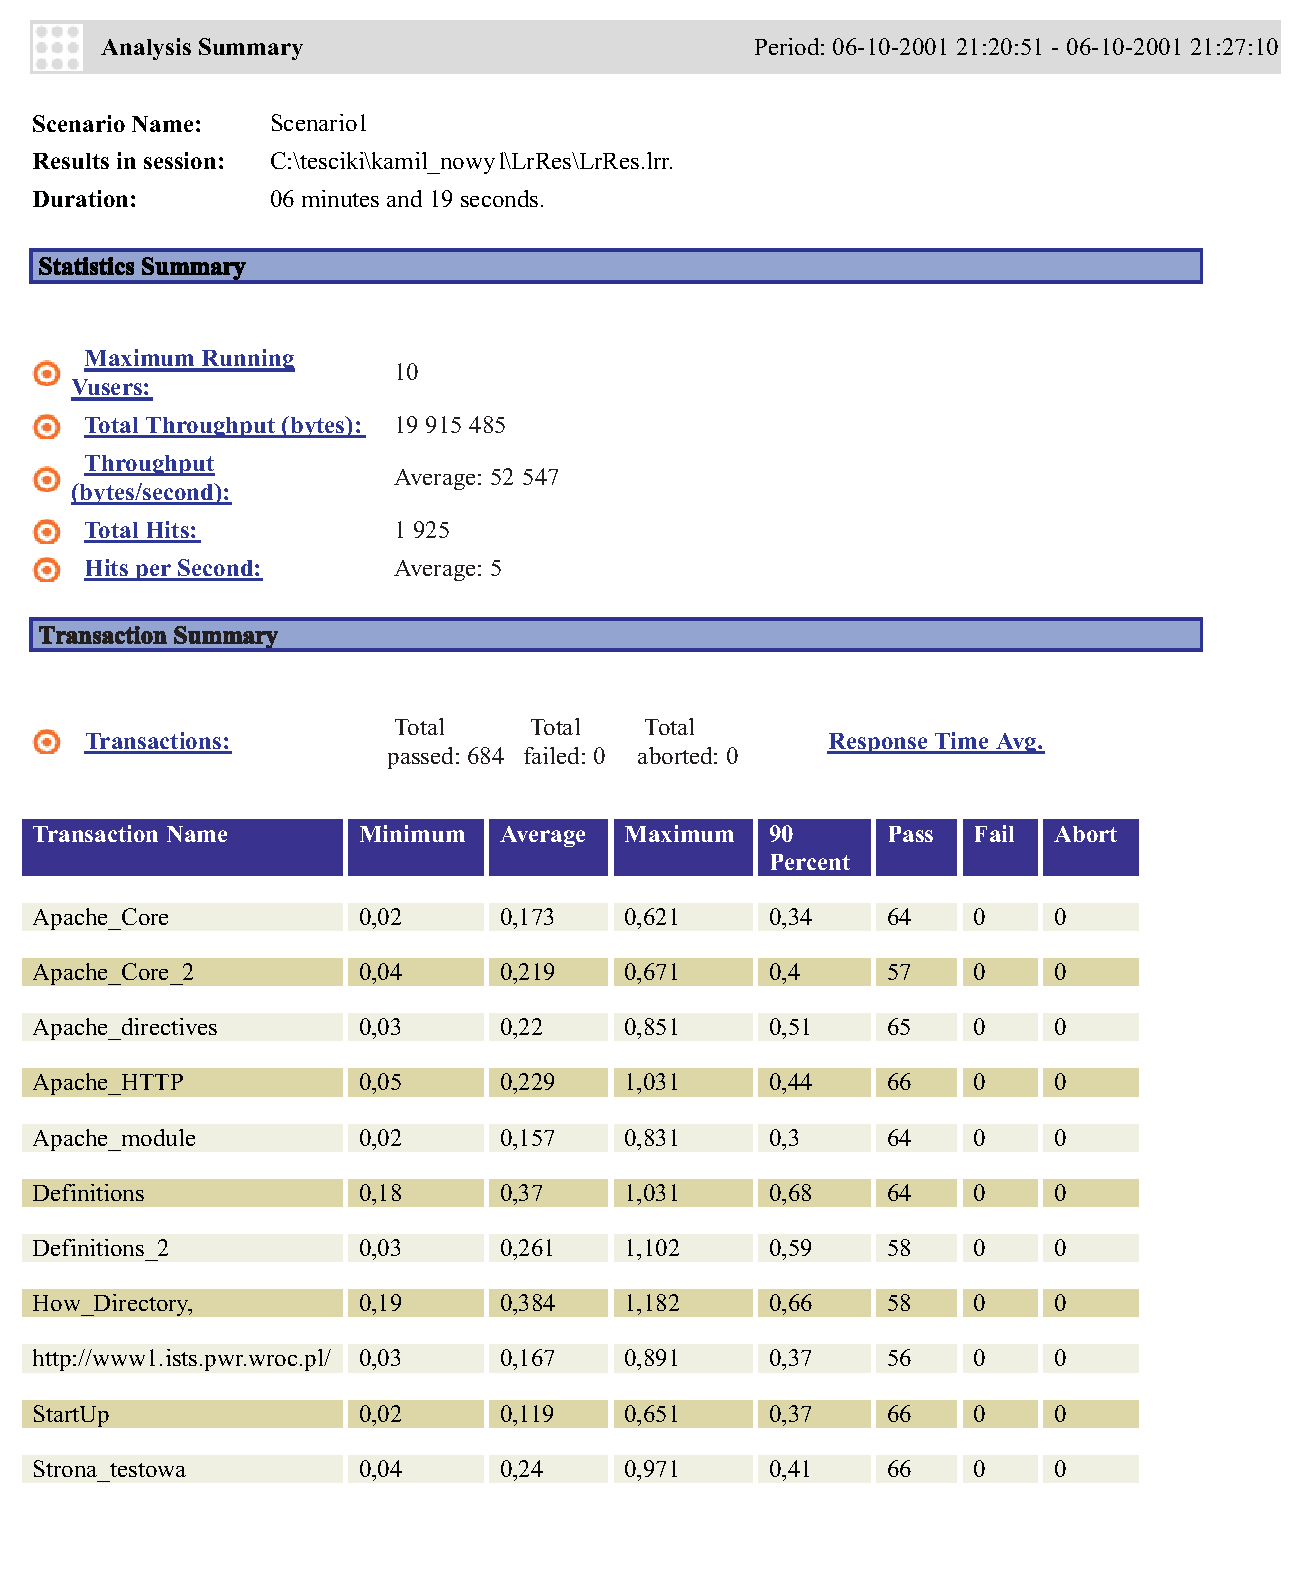
\includegraphics[width=\textwidth]{./rysunki/summary-test.eps}
\caption{Zebrane informacje o przebiegu testu}
\label{zebrane}
\end{figure}
\begin{figure}[h]
\centering

\includegraphics[width=4.5in]{./rysunki/raport1calybokiem.eps}
\caption{Wydajność wielokomputerowego systemu WWW}
\label{wydajnosc}
\end{figure}
\begin{figure}[h]
\centering

\includegraphics[width=4.5in]{./rysunki/raport2calybokiem.eps}
\caption{Ilość realizacji żądań na sekundę}
\label{zadania_sekunde}
\end{figure}
\begin{figure}[h]
\centering

\includegraphics[width=4.5in]{./rysunki/rapor3calybokiem.eps}
\caption{Ilość transakcji w zależności od pobieranej strony}
\label{pobierana_strona}
\end{figure}
\begin{figure}[h]
\centering
\includegraphics[width=\textwidth]{./rysunki/raport4calybokiem.eps}
\caption{Średni czas odpowiedzi}
\label{srednia_odpowiedz}
\end{figure}
\begin{figure}[h]
\centering
\includegraphics[width=4.5in]{./rysunki/raport7calybokiem.eps}
\caption{Zestawienie odpowiedzi w zależności od pobieranej strony}
\label{zestawienie_odpowiedzi}
\end{figure}
\begin{figure}[h]
\centering
\includegraphics[width=\textwidth]{./rysunki/raport9calybokiem.eps}
\caption{Czas odpowiedzi transakcji -- udział procentowy}
\label{procentowo}
\end{figure}
\begin{figure}[h]
\centering
\includegraphics[width=\textwidth]{./rysunki/raport10calybokiem.eps}
\caption{Czas odpowiedzi transakcji -- rozkład}
\label{odpowiedz_transakcji_rozklad}
\end{figure}
\begin{figure}[h]
\centering

\includegraphics[width=4.5in]{./rysunki/raport11calybokiem.eps}
\caption{Liczba stron na sekundę}
\label{stron_sekunda}
\end{figure}




\addcontentsline{toc}{chapter}{Literatura}
\bibliography{literatura}

\addcontentsline{toc}{chapter}{Spis Rysunków}
{\footnotesize\listoffigures}


\end{document}
